\documentclass{article}
\usepackage{graphicx}
\usepackage[hidelinks]{hyperref}
\usepackage{amsmath}
\usepackage{amssymb}
\usepackage{geometry}
\usepackage{booktabs}
\usepackage{enumitem}
\usepackage{float}
\usepackage{textcomp}
\usepackage{mdframed}
\usepackage[justification=centering]{caption}

\graphicspath{{figures/}}
\geometry{a4paper, margin=1in}

\title{A Practical Guide to Control Theory\\
\large For Engineering Students in Robot Competitions}
\author{Skywalker Liu\\
\href{mailto:ltx2499323877@outlook.com}{\texttt{ltx2499323877@outlook.com}} \quad\\
\quad
\href{https://github.com/liuskywalkerjskd}{\texttt{github.com/liuskywalkerjskd}}}
\date{October 2025}

\begin{document}

\maketitle

\newpage
\tableofcontents
\newpage

\input{sections/01_introduction}
\newpage

%=============================================================================
\section*{两个支配世界的数：$e$ 与 $\pi$}
\addcontentsline{toc}{section}{两个支配世界的数：$e$ 与 $\pi$}
%=============================================================================

在正式进入滤波器、传递函数和各种控制工具之前，让我们先花一点时间认识两个无理数——$\pi$ 和 $e$。它们悄无声息地支撑着这本笔记里几乎所有的公式。

你在高数课上见过它们，可能还背过小数点后好几位。但下面一句话就能概括\textit{它们在工程中为什么重要}：

\begin{mdframed}
\textbf{$\pi$ 是"重复"的语言。}\\
\textbf{$e$ 是"增长与衰减"的语言。}
\end{mdframed}

就这么简单。这本笔记里你将遇到的每一个方程，几乎都建立在这两个思想之上——或者同时建立在它们两个之上。

%---------------------------------------------------------------------
\subsection*{$\pi$：周期性的心跳}
%---------------------------------------------------------------------

转一个轮子，看一个钟摆来回摆动，听一根音叉嗡嗡作响——这些全是\textit{周期性}现象：同样的轨迹不断重复。而 $\pi$ 就是把圆的几何和重复的代数联系在一起的那个数。

想象一个点以匀速在单位圆上运动。它在 $t$ 时刻的水平坐标是 $\cos(t)$，垂直坐标是 $\sin(t)$。绕一整圈恰好需要 $2\pi$ 的时间。这不是巧合——这正是 $\pi$ 的来源。圆的周长是 $2\pi r$；除以半径就得到 $2\pi$，即旋转的"自然周期"。

在控制工程里，周期现象无处不在：机械结构的振动、电源的交流电压、欠阻尼阶跃响应中的振荡（系统超调后来回振荡、最终稳定下来的过程——后面会详细讲）、单片机的采样时钟——全都是周期性的。

\begin{figure}[H]
  \centering
  \includegraphics[width=\textwidth]{circle_sinusoid.pdf}
  \caption{单位圆上的一个点追踪出 $\cos t$ 与 $\sin t$。绕一整圈恰好 $2\pi$。}
\end{figure}

每当你写下 $\sin(\omega t)$ 或 $\cos(\omega t)$，$\pi$ 就藏在 $\omega = 2\pi f$ 里。傅里叶变换——我们分析信号的核心工具——把\textit{任意}信号分解成一系列正弦波的叠加，每一个正弦波都带着 $\pi$ 的因子。所以 $\pi$ 不只是关于圆的；它是"这个东西多久重复一次？"这个问题的通用语言。

%---------------------------------------------------------------------
\subsection*{$e$：增长与衰减的标尺}
%---------------------------------------------------------------------

现在换一个完全不同的场景：一个电容通过电阻放电。电压不会振荡——它只是慢慢减小。你每秒测一次，发现它总是损失\textit{剩余值的同一比例}。放射性衰变中的半衰期也是一样的道理：真正重要的不是绝对减少了多少，而是\textit{剩下了多大比例}。

这种"恒定比例变化"正是 $e$ 所刻画的。形式上，$e$ 是唯一满足 $f(x) = e^x$ 等于自身导数的底数：
\[
  \frac{d}{dx}\,e^{x} = e^{x}.
\]
用大白话说：$e^x$ 在任意一点的变化速度等于它当前的值。这使得 $e^x$ 成为"变化速度与当前状态成正比"这一方程的天然解——而这正是微分方程 $\dot{x} = ax$ 所描述的。

当 $a > 0$ 时，$x(t) = e^{at}$ 指数增长——像复利，像失稳系统一路狂飙。当 $a < 0$ 时，$x(t) = e^{at}$ 指数衰减——像那个正在放电的电容，像稳定系统慢慢回到平衡点。

\begin{figure}[H]
  \centering
  \includegraphics[width=0.75\textwidth]{exponential_growth_decay.pdf}
  \caption{指数曲线 $e^{at}$。$a>0$：不稳定增长；$a<0$：稳定衰减。}
\end{figure}

在控制理论中，$a$ 的正负（更精确地说，系统极点的实部）决定了稳定性的一切。极点在左半平面意味着 $e^{at}$（$a<0$）：响应会衰减。极点在右半平面意味着 $a>0$：响应会发散。就这一个想法——指数是在变大还是在变小——就是稳定性分析的全部基础。

到这里，$e$ 管衰减，$\pi$ 管振荡，两者泾渭分明。但真正让人拍案叫绝的是——它们其实可以合二为一。

%---------------------------------------------------------------------
\subsection*{当它们联手：$e^{j\theta}$}
%---------------------------------------------------------------------

真正的魔法发生在 $e$ 和 $\pi$ 相遇的时候。欧拉公式把它们绑在了一起：
\[
  e^{j\theta} = \cos\theta + j\sin\theta,
\]
其中 $j = \sqrt{-1}$。这个等式可以说是整个工程数学中最重要的恒等式。它告诉我们：\textit{复指数}同时既是指数函数又是正弦函数——增长/衰减和振荡，统一在一个表达式里。

当系统具有复数极点 $\sigma \pm j\omega$ 时，时域响应为
\[
  e^{\sigma t}\bigl(\cos\omega t + j\sin\omega t\bigr).
\]
其中 $e^{\sigma t}$（$e$ 的部分）控制\textbf{包络}——振荡是在增大、衰减还是保持不变；$\cos\omega t$（$\pi$ 的部分，因为 $\omega = 2\pi f$）控制\textbf{频率}——系统振荡得有多快。

\begin{figure}[H]
  \centering
  \includegraphics[width=0.82\textwidth]{damped_oscillation.pdf}
  \caption{阻尼振荡 $e^{\sigma t}\cos(\omega t)$：包络在衰减（$e$），信号在振荡（$\pi$）。}
\end{figure}

换句话说：\textbf{$e$ 告诉你衰减多快，$\pi$ 告诉你振荡多频}。这本笔记里你将研究的每一个二阶系统——从质量-弹簧-阻尼器到 PID 控制的电机——都不过是这两个数各司其职而已。

\vspace{1em}
\noindent $\pi$ 和 $e$ 已经就位，接下来的一切都有了根基。

\newpage

%=============================================================================
\section{Digital Signal Processing}
%=============================================================================

You might be wondering: ``I signed up for control theory, why are we starting with signal processing?'' Great question. Here is the answer: \textbf{garbage in, garbage out.}

Your controller is only as good as the data it receives. If your IMU reading is bouncing around like a caffeinated squirrel, no amount of PID tuning will save you. So before we learn to control systems, we learn to clean up their signals.

\subsection{Understanding the Frequency Domain}

In everyday life, we think about signals in the \textbf{time domain}---voltage changes over time, position changes over time. This is natural and intuitive. But it turns out that many problems become \textit{much} easier if we look at signals from a different angle: the \textbf{frequency domain}.

The core idea is beautifully simple: \textit{any signal can be decomposed into a sum of sinusoids of different frequencies.} Your noisy gyroscope reading? It is actually a clean low-frequency rotation signal plus a bunch of high-frequency noise signals all added together. If we can identify which frequencies are ``signal'' and which are ``noise,'' we can surgically remove the noise.

Think of it like an audio equalizer on a music player. The bass, mids, and treble are all mixed together in the time-domain waveform. But the equalizer lets you boost or cut specific frequency ranges independently. That is exactly what we do with filters in control systems.

\textbf{Key intuition:} Slow, meaningful changes in your system (like a chassis turning) happen at low frequencies. Fast, meaningless changes (like electrical noise or vibration) happen at high frequencies. The frequency domain lets us tell them apart.

\subsection{Laplace Transform and Fourier Transform}

These two transforms are your tickets from the time domain to the frequency domain. They are closely related, but they serve slightly different purposes.

\subsubsection{Laplace Transform}

The Laplace transform takes a time-domain function $f(t)$ and converts it into a function of the complex variable $s$:

\begin{equation}
F(s) = \mathcal{L}\{f(t)\} = \int_0^{\infty} f(t) e^{-st} \, dt
\end{equation}

where $s = \sigma + j\omega$ is a complex number. The real part $\sigma$ captures exponential growth or decay, and the imaginary part $j\omega$ captures oscillation.

\textbf{Why do we care?} Because the Laplace transform turns differential equations into algebraic equations. Instead of solving
\[
m\ddot{x} + b\dot{x} + kx = F(t),
\]
(which requires calculus), we can solve
\[
(ms^2 + bs + k)X(s) = F(s),
\]
(which is just algebra). Derivatives become multiplication by $s$. Integration becomes division by $s$. Life becomes easier.

The most important Laplace transforms you will use daily:

\begin{center}
\begin{tabular}{lll}
\toprule
\textbf{Time domain} & \textbf{$s$-domain} & \textbf{When you see it} \\
\midrule
$1$ (step input) & $\frac{1}{s}$ & Commanding a new setpoint \\
$e^{-at}$ & $\frac{1}{s+a}$ & First-order system response \\
$\sin(\omega t)$ & $\frac{\omega}{s^2 + \omega^2}$ & Oscillation, vibration \\
$\dot{f}(t)$ & $sF(s) - f(0)$ & Derivative in the controller \\
$\int f(t)\,dt$ & $\frac{F(s)}{s}$ & Integral in the controller \\
\bottomrule
\end{tabular}
\end{center}

\textbf{Pro tip:} You do not need to memorize the integral formula. You need to understand that $s$ means ``derivative'' and $1/s$ means ``integral.'' That single insight will carry you through 80\% of control theory.

\textbf{What is $e^{-st}$ actually doing?} The kernel $e^{-st} = e^{-\sigma t} e^{-j\omega t}$ is a ``probe signal'' that asks two questions simultaneously: (1) $e^{-\sigma t}$: ``Does the signal grow or decay at rate $\sigma$?'' (2) $e^{-j\omega t}$: ``How much of frequency $\omega$ is present?'' By integrating $f(t) \cdot e^{-st}$ over all time, we compute the ``correlation'' between the signal and every possible exponential-sinusoid. The result $F(s)$ is a map of the entire complex plane, telling us exactly how much of each exponential-oscillatory mode exists in the signal.

\textbf{Common Laplace transform pairs --- worked out:}

The \textbf{unit step} $u(t) = 1$ for $t \geq 0$:
\[
\mathcal{L}\{1\} = \int_0^{\infty} e^{-st} \, dt = \left[-\frac{e^{-st}}{s}\right]_0^{\infty} = \frac{1}{s}
\]

The \textbf{exponential decay} $e^{-at}$:
\[
\mathcal{L}\{e^{-at}\} = \int_0^{\infty} e^{-at} e^{-st} \, dt = \int_0^{\infty} e^{-(s+a)t} \, dt = \frac{1}{s+a}
\]
This is why a first-order system with pole at $s = -a$ has a time response of $e^{-at}$---the pole location \textit{is} the decay rate.

The \textbf{ramp} $t \cdot u(t)$:
\[
\mathcal{L}\{t\} = \frac{1}{s^2}
\]
Notice: multiplying by $t$ in time corresponds to differentiating with respect to $s$ and flipping the sign: $\mathcal{L}\{t \cdot f(t)\} = -\frac{d}{ds}F(s)$. Since $\mathcal{L}\{1\} = 1/s$, we get $\mathcal{L}\{t\} = -\frac{d}{ds}\frac{1}{s} = \frac{1}{s^2}$.

\subsubsection{Fourier Transform}

The Fourier transform is the Laplace transform's well-behaved cousin. It is what you get when you set $s = j\omega$ (i.e., $\sigma = 0$):

\begin{equation}
F(j\omega) = \int_{-\infty}^{\infty} f(t) e^{-j\omega t} \, dt
\end{equation}

While the Laplace transform works with the full complex plane (and can handle unstable, growing signals), the Fourier transform lives strictly on the imaginary axis. It tells you: ``How much of each frequency is present in this signal?''

\textbf{When to use which:}
\begin{itemize}
    \item \textbf{Laplace transform}: For analyzing and designing control systems (transfer functions, stability).
    \item \textbf{Fourier transform}: For analyzing signals (noise, vibration, frequency content).
\end{itemize}

In practice, for digital systems we often use the \textbf{Discrete Fourier Transform (DFT)}, computed efficiently via the \textbf{Fast Fourier Transform (FFT)} algorithm. If you ever want to see what frequencies are hiding in your sensor data, just throw it into an FFT. MATLAB's \texttt{fft()} or Python's \texttt{numpy.fft.fft()} will do the job in one line.

\subsubsection{Frequency Spectrum}

When you apply the Fourier transform to a signal, you get its \textbf{frequency spectrum}---a plot showing the amplitude (and phase) of each frequency component.

Reading a frequency spectrum is like reading an X-ray of your signal:
\begin{itemize}
    \item A tall peak at 50 Hz? That is probably power line interference.
    \item A broad hump below 10 Hz? That is likely your actual signal of interest.
    \item Random fuzz spread across all frequencies? That is white noise.
\end{itemize}

\textbf{Practical example:} Suppose your gimbal encoder gives a noisy velocity reading. You record 1 second of data, compute the FFT, and see a clean peak at 3 Hz (your gimbal is tracking a target moving at 3 Hz) plus a mess of noise above 50 Hz. Now you know: design a low-pass filter with a cutoff around 20--30 Hz, and your signal will be clean.

The frequency spectrum has two parts:
\begin{itemize}
    \item \textbf{Magnitude spectrum} $|F(j\omega)|$: How strong each frequency component is.
    \item \textbf{Phase spectrum} $\angle F(j\omega)$: The time shift of each frequency component.
\end{itemize}

For filter design, we mostly care about the magnitude spectrum. Phase becomes important later when we analyze control loop stability (phase margin).

\begin{figure}[H]
\centering
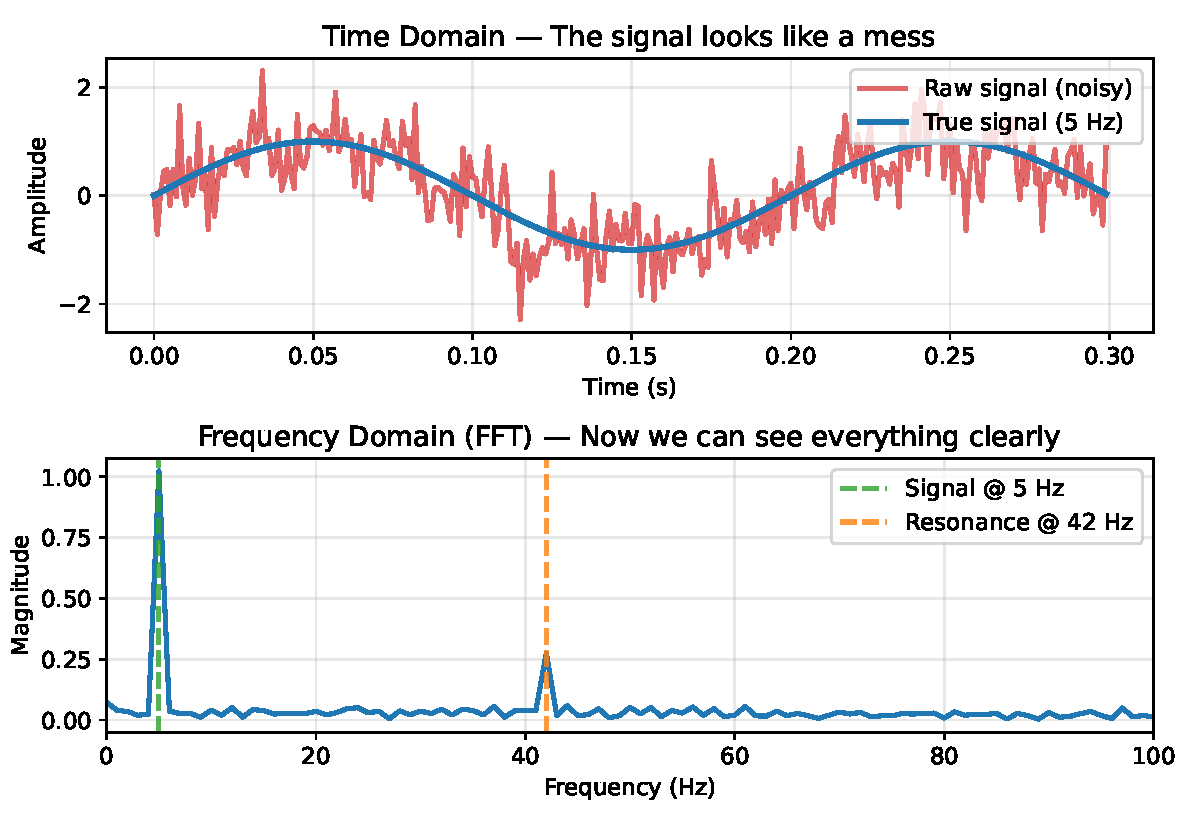
\includegraphics[width=\textwidth]{frequency_spectrum.pdf}
\caption{Top: a noisy time-domain signal looks hopeless. Bottom: the FFT instantly reveals a 5 Hz signal and a 42 Hz resonance hiding in the noise.}
\end{figure}

\vspace{0.5em}
\begin{mdframed}[linewidth=1pt, innertopmargin=10pt, innerbottommargin=10pt]
\textbf{Case Study: Debugging a Vibrating Chassis with FFT}

\vspace{0.3em}
True story pattern from competition robotics: Your mecanum chassis drives fine at low speed but develops a nasty vibration at high speed. The whole frame buzzes. Everyone suspects a loose screw. You tighten everything. Still vibrates.

\textbf{The diagnosis:} Log the IMU accelerometer data for 5 seconds while driving at the problematic speed. Run an FFT in Python:

\begin{verbatim}
    import numpy as np
    freqs = np.fft.rfftfreq(len(data), d=1.0/sample_rate)
    spectrum = np.abs(np.fft.rfft(data))
    plt.plot(freqs, spectrum)
\end{verbatim}

You see a massive spike at exactly 42 Hz. Interesting. You calculate: at high speed, the mecanum wheel rollers contact the ground at\ldots about 42 Hz. The roller contact frequency matches a structural resonance of the chassis frame.

\textbf{The fix options:}
\begin{itemize}[nosep]
    \item Add a \textbf{notch filter} (band-reject) at 42 Hz in the control loop to prevent the controller from exciting the resonance.
    \item Add physical damping (rubber mounts) to shift the resonance frequency.
    \item Stiffen the frame to move the resonance above the operating range.
\end{itemize}

\textbf{The lesson:} Without the FFT, you would have spent hours tightening screws. With the FFT, the root cause was obvious in 10 seconds. \textbf{The frequency domain is a debugging superpower.} Whenever something oscillates and you do not know why, record the data and look at the spectrum.
\end{mdframed}

\subsection{Frequency-Based Filter Design}

Now that we can see signals in the frequency domain, we can design filters to keep the frequencies we want and reject the ones we do not.

A filter is simply a system that has different gains at different frequencies. We describe this using the filter's \textbf{frequency response}---a plot of gain vs.\ frequency (called a \textbf{Bode magnitude plot}).

\subsubsection{Low-Pass Filter}

The most common filter in robotics. It passes low frequencies and attenuates high frequencies.

\textbf{First-order low-pass filter:}
\begin{equation}
H(s) = \frac{\omega_c}{s + \omega_c}
\end{equation}

where $\omega_c = 2\pi f_c$ is the cutoff frequency in rad/s. At frequencies below $\omega_c$, the gain is approximately 1 (signal passes through). Above $\omega_c$, the gain rolls off at $-20$ dB/decade (signal gets attenuated).

\textbf{In the time domain}, this is equivalent to an exponential moving average:
\begin{equation}
y[n] = \alpha \cdot x[n] + (1 - \alpha) \cdot y[n-1]
\end{equation}

where $\alpha = \frac{T_s}{T_s + \frac{1}{2\pi f_c}}$ and $T_s$ is the sampling period.

\textbf{When to use:} Smoothing noisy sensor readings (gyroscope, accelerometer, motor current). This is the filter you will use 90\% of the time.

\textbf{Gotcha:} A low-pass filter introduces \textbf{phase lag}---the output is delayed relative to the input. The more aggressively you filter (lower cutoff), the more lag you introduce. In a fast control loop, this lag can destabilize your system. There is always a trade-off between smooth signals and fast response.

\begin{figure}[H]
\centering
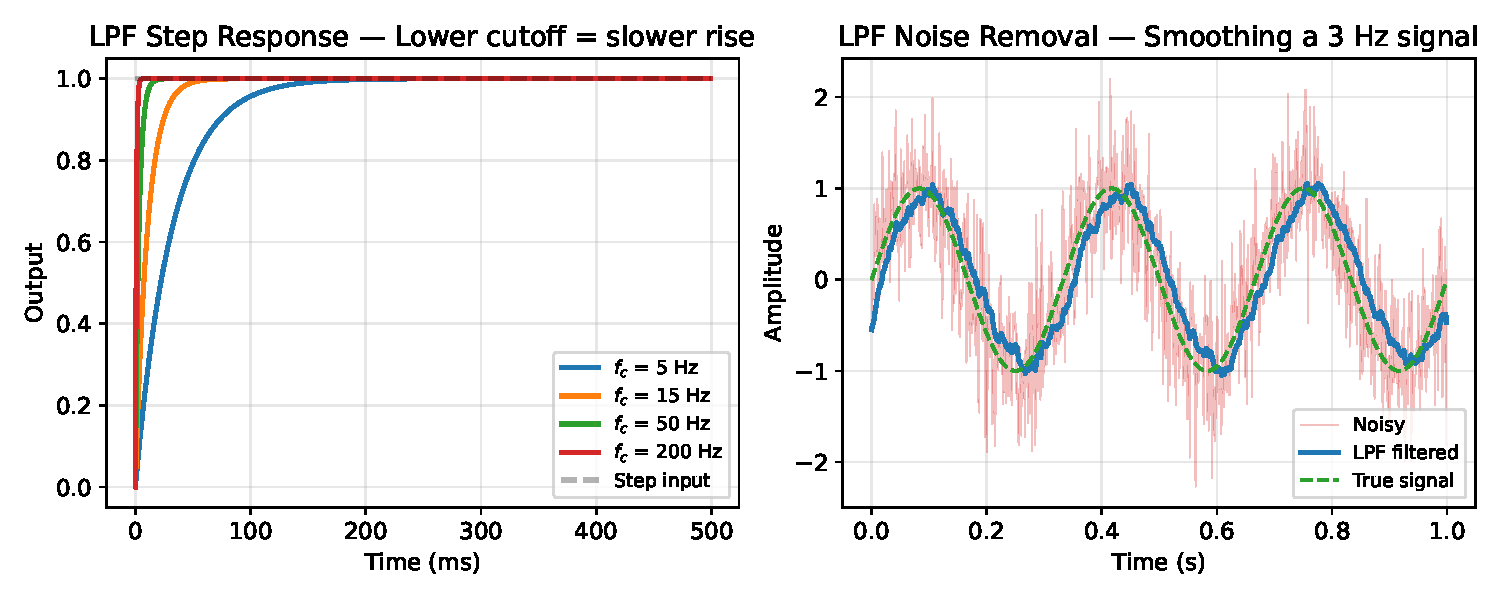
\includegraphics[width=\textwidth]{lpf_response.pdf}
\caption{Left: LPF step response --- lower cutoff means slower rise but smoother output. Right: filtering a noisy 3 Hz signal --- the LPF recovers the true signal while removing high-frequency noise.}
\end{figure}

\vspace{0.5em}
\begin{mdframed}[linewidth=1pt, innertopmargin=10pt, innerbottommargin=10pt]
\textbf{Case Study: Why a Low-Pass Filter Gives You ``Soft Start'' for Free}

\vspace{0.3em}
Suppose you command your motor to jump from 0 to 5000 RPM instantly (a step input). Without any filter, the setpoint changes discontinuously---the motor driver sees a sudden full-voltage command, the gears slam, the chassis lurches, and your teammates spill their coffee.

Now insert a first-order LPF on the setpoint: $r_{\text{filtered}}(s) = \frac{\omega_c}{s + \omega_c} \cdot R(s)$. What happens?

The step input in the $s$-domain is $R(s) = \frac{5000}{s}$. After the filter:
\[
R_{\text{filtered}}(s) = \frac{5000 \, \omega_c}{s(s + \omega_c)}
\]

Taking the inverse Laplace transform:
\[
r_{\text{filtered}}(t) = 5000 \left(1 - e^{-\omega_c t}\right)
\]

The step has been transformed into a \textbf{smooth exponential ramp}. The time constant is $\tau = 1/\omega_c$. After $3\tau$, the output reaches 95\% of the target; after $5\tau$, it is at 99\%.

\textbf{Why this matters on your robot:}
\begin{itemize}[nosep]
    \item \textbf{Mechanical protection:} Gears and belts have torque limits. A step command can strip teeth or snap belts. The LPF limits the rate of change, keeping forces within safe bounds.
    \item \textbf{Current limiting:} A sudden voltage step causes a huge inrush current ($I = V/R$ when back-EMF is still zero). The LPF ramps up the voltage gradually, keeping current manageable.
    \item \textbf{Tunable aggressiveness:} Want a faster ramp? Increase $\omega_c$ (higher cutoff). Want a gentler ramp? Decrease $\omega_c$. One parameter controls the entire behavior.
\end{itemize}

\textbf{Comparison with a linear ramp:} You could also ramp the setpoint linearly (e.g., increase by 1000 RPM/s). But the LPF is better because it also smooths out \textit{any} discontinuity in the setpoint---not just the initial step, but also sudden changes during operation. It is a ``set it and forget it'' solution.

\textbf{The code is trivial:}
\begin{verbatim}
    setpoint_filtered += alpha * (setpoint_raw - setpoint_filtered);
\end{verbatim}

One line of code. No lookup tables, no state machines. That is the beauty of the LPF as a soft-start mechanism.
\end{mdframed}

\begin{figure}[H]
\centering
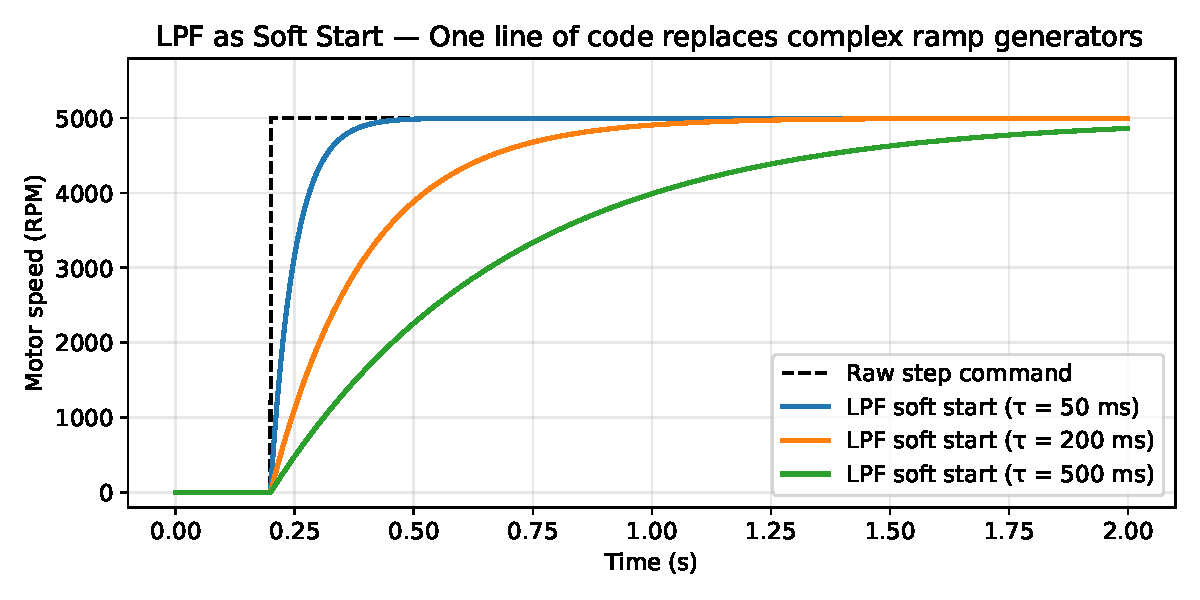
\includegraphics[width=\textwidth]{lpf_soft_start.pdf}
\caption{LPF soft start: a single parameter $\tau$ controls how aggressively the motor ramps up. The step command becomes a smooth exponential curve.}
\end{figure}

\subsubsection{Band-Pass Filter}

Passes a specific range of frequencies and attenuates everything else. Think of it as a low-pass and a high-pass filter combined.

\begin{equation}
H(s) = \frac{\frac{\omega_0}{Q} s}{s^2 + \frac{\omega_0}{Q} s + \omega_0^2}
\end{equation}

where $\omega_0$ is the center frequency and $Q$ is the quality factor (higher $Q$ = narrower band).

\textbf{When to use:} Extracting a specific frequency component from a signal. For example, if you know your target oscillates at a specific frequency and you want to track it while rejecting everything else.

In robotics, band-pass filters are less common than low-pass filters, but they are useful for vibration analysis and resonance detection.

\subsubsection{High-Pass Filter}

Passes high frequencies, attenuates low frequencies. It is the opposite of a low-pass filter.

\textbf{First-order high-pass filter:}
\begin{equation}
H(s) = \frac{s}{s + \omega_c}
\end{equation}

\textbf{When to use:} Removing DC offset or slow drift from a signal. For example, if your accelerometer has a slowly drifting bias, a high-pass filter can remove it while keeping the fast acceleration data intact.

\textbf{Practical note:} A complementary filter (commonly used for IMU sensor fusion) is just a low-pass filter on one sensor and a high-pass filter on another, with their cutoff frequencies matched so the gains add up to 1. The accelerometer gets low-passed (trust it for slow/static orientation) and the gyroscope gets high-passed (trust it for fast rotations). Simple, elegant, and surprisingly effective.

\subsubsection{Filter Type Selection and Parameter Tuning}

Choosing the right filter comes down to answering three questions:
\begin{enumerate}
    \item \textbf{What frequencies do I want to keep?} This determines the filter type (low-pass, high-pass, band-pass).
    \item \textbf{Where is the boundary?} This determines the cutoff frequency $f_c$.
    \item \textbf{How sharp should the transition be?} This determines the filter order.
\end{enumerate}

\textbf{Rules of thumb:}
\begin{itemize}
    \item Start with a first-order low-pass filter. It is simple, stable, and good enough for most applications.
    \item Set the cutoff frequency to 5--10$\times$ the bandwidth of your signal of interest. Too low and you lose signal; too high and you keep noise.
    \item If a first-order filter is not enough, try second-order (Butterworth for flat passband, Chebyshev for sharper rolloff).
    \item \textbf{Never} design a filter without looking at the frequency spectrum of your actual data first. Guessing cutoff frequencies is a recipe for frustration.
    \item When in doubt, plot the filtered output alongside the raw signal and check if the result makes physical sense.
\end{itemize}

\subsubsection{Digital Filter Structures: FIR vs.\ IIR}

So far we have described filters using continuous-time transfer functions $H(s)$.
Once you discretize them (covered in detail in Section~5), you end up with one of
two fundamental digital filter structures: \textbf{FIR} and \textbf{IIR}.
Understanding the difference is essential for choosing the right implementation on
your microcontroller.

\paragraph{FIR (Finite Impulse Response).}
An FIR filter computes the output as a weighted sum of the current and past input
samples only---no feedback:

\begin{equation}
y[n] = \sum_{k=0}^{M} b_k \, x[n-k]
\end{equation}

In the $z$-domain:
\begin{equation}
H(z) = \sum_{k=0}^{M} b_k \, z^{-k}
\end{equation}

FIR filters have \textbf{only zeros} (no poles except trivially at $z = 0$), which
gives them two important properties:
\begin{itemize}
    \item \textbf{Always stable}---no feedback means no risk of runaway oscillation.
    \item \textbf{Linear phase} is achievable by making the coefficients symmetric
          ($b_k = b_{M-k}$). This means every frequency component is delayed by the
          same amount, so the signal shape is perfectly preserved.
\end{itemize}

The price you pay is \textbf{filter order}: to get a sharp cutoff you may need
$M = 50$--$200$ taps, which means storing that many past samples and performing
that many multiplications per output sample.

\textbf{Common FIR design methods:}
\begin{itemize}
    \item \textbf{Window method}---truncate the ideal impulse response and apply a
          window function (Hamming, Blackman, Kaiser) to reduce spectral leakage.
    \item \textbf{Frequency sampling}---specify the desired magnitude response at
          DFT sample points and inverse-transform.
    \item \textbf{Parks--McClellan (Remez)}---an optimal algorithm that minimizes
          the maximum approximation error (equiripple design).
\end{itemize}

\paragraph{IIR (Infinite Impulse Response).}
An IIR filter uses \textit{both} past inputs and past outputs---it has a feedback path:

\begin{equation}
y[n] = \sum_{k=0}^{M} b_k \, x[n-k] \;-\; \sum_{k=1}^{N} a_k \, y[n-k]
\end{equation}

In the $z$-domain:
\begin{equation}
H(z) = \frac{\displaystyle\sum_{k=0}^{M} b_k \, z^{-k}}
            {1 + \displaystyle\sum_{k=1}^{N} a_k \, z^{-k}}
     = \frac{B(z)}{A(z)}
\end{equation}

IIR filters have \textbf{both poles and zeros}. The poles enable sharp frequency
selectivity with very low order (a 4th-order IIR can outperform a 50th-order FIR),
but they come with risks:
\begin{itemize}
    \item \textbf{Potentially unstable}---if any pole lies outside the unit circle
          ($|z| > 1$), the output grows without bound.
    \item \textbf{Nonlinear phase}---different frequencies are delayed by different
          amounts, which distorts the signal shape.
    \item \textbf{Coefficient sensitivity}---on fixed-point microcontrollers,
          rounding the coefficients can shift poles enough to cause instability.
\end{itemize}

\textbf{Classical IIR design} starts from an analog prototype and maps it to
discrete time:
\begin{itemize}
    \item \textbf{Butterworth}---maximally flat passband, monotonic rolloff. The
          ``vanilla'' choice; sounds boring but is the right default 80\% of the time.
    \item \textbf{Chebyshev Type~I}---equiripple in the passband, monotonic in the
          stopband. Sharper transition than Butterworth for the same order, at the
          cost of passband ripple.
    \item \textbf{Chebyshev Type~II}---monotonic in the passband, equiripple in the
          stopband. Less common but useful when passband flatness matters more.
    \item \textbf{Elliptic (Cauer)}---equiripple in \textit{both} bands. Gives the
          sharpest possible transition for a given filter order, but with ripple
          everywhere.
\end{itemize}

The two main analog-to-digital mappings are:
\begin{itemize}
    \item \textbf{Bilinear transform}: $z = \dfrac{1 + (sT_s/2)}{1 - (sT_s/2)}$.
          This is the workhorse method. It maps the entire $j\omega$ axis onto the
          unit circle with no aliasing, but introduces \textit{frequency warping}:
          analog frequencies get compressed near the Nyquist frequency.
          You compensate by \textbf{pre-warping} the critical frequencies before
          designing the analog prototype.
    \item \textbf{Impulse invariance}: $h[n] = T_s \cdot h_a(nT_s)$.
          Preserves the time-domain impulse response, but suffers from
          \textit{aliasing} if the analog filter is not sufficiently band-limited.
          Mainly used for low-pass and band-pass designs.
\end{itemize}

\paragraph{Head-to-head comparison.}

\begin{center}
\begin{tabular}{lll}
\toprule
\textbf{Property} & \textbf{FIR} & \textbf{IIR} \\
\midrule
Stability & Always stable & Must verify (poles inside unit circle) \\
Phase & Linear phase achievable & Nonlinear phase \\
Order for sharp cutoff & High (50--200+) & Low (4--10 typical) \\
Computation per sample & $M+1$ multiplies & $M+N+1$, but $M,N$ are small \\
Latency & Higher (longer filter) & Lower \\
Design from analog prototype & No & Yes \\
Coefficient sensitivity & Low & High \\
\bottomrule
\end{tabular}
\end{center}

\paragraph{Practical guidelines.}
\begin{itemize}
    \item Need \textbf{linear phase} (audio, symmetric pulse shaping, communications)?
          Use \textbf{FIR}.
    \item Need a \textbf{sharp cutoff with minimal computation} (real-time control
          loops, resource-constrained MCUs)? Use \textbf{IIR}.
    \item Need \textbf{guaranteed stability} without careful analysis? Use
          \textbf{FIR}.
    \item For higher-order IIR filters, \textbf{always} implement as cascaded
          second-order sections (biquads) to reduce coefficient sensitivity:
\end{itemize}
\begin{equation}
H(z) = \prod_{i=1}^{L}
       \frac{b_{0i} + b_{1i}\,z^{-1} + b_{2i}\,z^{-2}}
            {1   + a_{1i}\,z^{-1} + a_{2i}\,z^{-2}}
\end{equation}

Each section is a ``biquad''---a second-order IIR filter that is simple to
implement and numerically well-behaved. Cascading $L$ biquads gives you a
$2L$-th order filter while keeping coefficient quantization effects local to each
section.

\textbf{Example: a biquad in C}
\begin{verbatim}
    // One biquad section
    float biquad(float x, float *state,
                 float b0, float b1, float b2,
                 float a1, float a2) {
        float y = b0*x + state[0];
        state[0] = b1*x - a1*y + state[1];
        state[1] = b2*x - a2*y;
        return y;
    }
\end{verbatim}

This is the \textbf{transposed direct-form~II} structure---two state variables per
biquad, numerically stable, and the standard choice for floating-point
implementations.

\vspace{0.5em}
\begin{mdframed}[linewidth=1pt, innertopmargin=10pt, innerbottommargin=10pt]
\textbf{Quick Decision Flowchart}

\vspace{0.3em}
\begin{enumerate}[nosep]
    \item Is the application phase-sensitive (e.g., symmetric waveform matters)?
          $\rightarrow$ \textbf{FIR} with symmetric coefficients.
    \item Is real-time computation tight (MCU running a fast control loop)?
          $\rightarrow$ \textbf{IIR} (Butterworth or Chebyshev), implemented as
          cascaded biquads.
    \item Is the filter order moderate and your platform has enough memory?
          $\rightarrow$ Either works; default to \textbf{FIR} for simplicity and
          robustness.
    \item Do you need the sharpest possible transition band for a given order?
          $\rightarrow$ \textbf{IIR} with an Elliptic prototype.
\end{enumerate}

\textbf{Rule of thumb for robotics:} Most sensor-smoothing filters on embedded
systems are low-order IIR (often just 1st or 2nd order Butterworth). FIR filters
shine in audio processing, communications, and any application where linear phase
is non-negotiable.
\end{mdframed}

\subsection{Z-Transform}

Everything we have discussed so far with the Laplace transform lives in the continuous world. But your microcontroller is digital---it works with samples, not continuous signals. The \textbf{Z-transform} is the discrete-time equivalent of the Laplace transform.

The Z-transform of a discrete sequence $x[n]$ is:
\begin{equation}
X(z) = \sum_{n=0}^{\infty} x[n] z^{-n}
\end{equation}

The key correspondence is:
\begin{center}
\begin{tabular}{ll}
\toprule
\textbf{Continuous ($s$-domain)} & \textbf{Discrete ($z$-domain)} \\
\midrule
$s$ (derivative) & $\frac{z-1}{T_s}$ (forward difference) \\
$\frac{1}{s}$ (integral) & $\frac{T_s}{z-1}$ (accumulator) \\
Stable if $\text{Re}(s) < 0$ & Stable if $|z| < 1$ \\
$e^{-aT_s}$ in $s$-domain & $z^{-1}$ is one-sample delay \\
\bottomrule
\end{tabular}
\end{center}

\textbf{Why do we care?} Because when you implement a filter or controller on a microcontroller, you are working in the $z$-domain, whether you realize it or not. That simple line of code:
\[
\texttt{y = alpha * x + (1 - alpha) * y\_prev;}
\]
is actually a $z$-domain transfer function:
\[
H(z) = \frac{\alpha}{1 - (1-\alpha)z^{-1}}
\]

Understanding the Z-transform helps you:
\begin{itemize}
    \item Convert continuous-time filters/controllers to code (covered in Section 5).
    \item Analyze the stability of your discrete-time system.
    \item Understand why your controller might behave differently at different sampling rates.
\end{itemize}

For now, just remember: \textbf{$z^{-1}$ means ``one time step ago.''} That is the single most important thing about the Z-transform.

\textbf{Common Z-transform pairs:}

\begin{center}
\begin{tabular}{lll}
\toprule
\textbf{Discrete signal} & \textbf{$z$-domain} & \textbf{When you see it} \\
\midrule
$\delta[n]$ (unit impulse) & $1$ & Initial kick \\
$u[n]$ (unit step) & $\frac{z}{z-1}$ & Step command \\
$a^n u[n]$ (geometric decay) & $\frac{z}{z-a}$ & Discrete first-order response \\
$x[n-1]$ (one-step delay) & $z^{-1}X(z)$ & Previous sample in code \\
$x[n] - x[n-1]$ (first difference) & $(1 - z^{-1})X(z)$ & Discrete derivative \\
$\sum_{k=0}^{n} x[k]$ (running sum) & $\frac{1}{1 - z^{-1}}X(z)$ & Discrete integral \\
\bottomrule
\end{tabular}
\end{center}

\textbf{The connection between $s$ and $z$:} The exact mapping is $z = e^{sT_s}$. A continuous pole at $s = -a$ maps to a discrete pole at $z = e^{-aT_s}$. This means:
\begin{itemize}
    \item A stable continuous pole ($\text{Re}(s) < 0$) maps to $|z| < 1$ (inside the unit circle). Stability is preserved.
    \item A faster continuous pole (more negative $s$) maps to a smaller $|z|$ (closer to the origin). Very fast poles map near $z = 0$.
    \item An oscillatory continuous pole ($s = \sigma \pm j\omega$) maps to $z = e^{\sigma T_s} e^{\pm j\omega T_s}$, which spirals inside (stable) or outside (unstable) the unit circle.
\end{itemize}

\textbf{Reading a $z$-domain transfer function:} Any $z$-domain transfer function can be directly translated to code by replacing $z^{-1}$ with ``previous value.'' For example:
\[
H(z) = \frac{b_0 + b_1 z^{-1}}{1 + a_1 z^{-1}}
\]
becomes:
\begin{verbatim}
    y = b0 * x + b1 * x_prev - a1 * y_prev;
    x_prev = x;  y_prev = y;
\end{verbatim}
This is called a \textbf{difference equation}, and it is the final form of any digital filter or controller.

\newpage

\input{sections/03_system_description}
\newpage

%=============================================================================
\section{经典控制理论}
%=============================================================================

终于到了你最想看的章节。经典控制理论讲的就是怎么让系统听话。而经典控制的绝对主角——95\% 的比赛机器人都在用的工具——就是 PID 控制器。

不过在讲 PID 之前，得先搞清楚反馈控制为什么管用。

\subsection{反馈控制的基本概念}

\textbf{开环控制}就像闷头做菜不尝味道。严格按菜谱操作，祈祷结果没问题。烤箱温度偏了 10 度？蛋糕废了。

\textbf{闭环（反馈）控制}就像边做边尝。尝一口，调味，再尝，再调。烤箱温度不准也没关系，因为你在实时补偿。

用数学语言描述，一个基本的反馈回路如下：

\begin{enumerate}
    \item 计算\textbf{误差（error）}：$e(t) = r(t) - y(t)$，其中 $r$ 是期望输出（设定值），$y$ 是实际输出。
    \item 将误差输入\textbf{控制器（controller）} $C(s)$，产生控制输入 $u(t)$。
    \item 控制输入驱动\textbf{被控对象（plant）} $G(s)$，产生输出 $y(t)$。
    \item 测量 $y(t)$，返回第1步。
\end{enumerate}

从设定值 $R$ 到输出 $Y$ 的闭环传递函数（Closed-loop Transfer Function）为：

从框图出发：误差 $E(s) = R(s) - Y(s)$，控制器输出 $U(s) = C(s)E(s)$，被控对象输出 $Y(s) = G(s)U(s)$。组合得 $Y = GC(R - Y)$，整理：$Y(1 + GC) = GCR$，故：
\begin{equation}
\frac{Y(s)}{R(s)} = \frac{C(s)G(s)}{1 + C(s)G(s)}
\end{equation}

经典控制里最重要的一个公式。多看两眼，记住它。

\textbf{解析闭环传递函数：}

令 $L(s) = C(s)G(s)$ 为\textbf{回路传递函数（loop transfer function）}（也叫开环传递函数）。则：

\begin{itemize}
    \item \textbf{互补灵敏度函数（Complementary Sensitivity，设定值跟踪）}：$T(s) = \frac{L(s)}{1 + L(s)}$。这就是上面写的那个——它告诉你输出跟随参考的好坏程度。理想情况下，$T(s) \approx 1$（低频处跟踪良好），$T(s) \approx 0$（高频处抑制噪声）。

    \item \textbf{灵敏度函数（Sensitivity Function）}：$S(s) = \frac{1}{1 + L(s)}$。它告诉你输出端的扰动对输出的影响程度。$S$ 越小 = 抗扰性越好。注意 $T(s) + S(s) = 1$ 始终成立——你\textit{不可能}在同一频率下同时实现完美跟踪和完美抗扰。这是反馈控制的基本局限。

    \item \textbf{输入灵敏度（Input Sensitivity）}：$C(s) \cdot S(s) = \frac{C(s)}{1 + L(s)}$。它告诉你需要多大的控制量。如果这个量在高频处很大，你的执行器就会没日没夜地放大噪声。
\end{itemize}

\textbf{一句话抓住要害：}回路增益大（$|L(j\omega)| \gg 1$）的频段内，$T \approx 1$，$S \approx 0$——反馈在干活。回路增益小（$|L(j\omega)| \ll 1$）的频段内，$T \approx 0$，$S \approx 1$——反馈摆烂。\textbf{带宽（bandwidth）}就是 $|L(j\omega)| = 1$（穿越频率）对应的频率，是"反馈管用"和"反馈不管用"的分界线。

\textbf{反馈凭什么这么强：}
\begin{itemize}
    \item \textbf{不怕模型不准。}$G(s)$ 和实际有出入？反馈能兜底。
    \item \textbf{自动抗扰。}摩擦、风、碰撞——来一个纠一个。
    \item \textbf{重塑动态响应。}选对 $C(s)$，系统可以更快、阻尼可以更足。
\end{itemize}

\textbf{代价：}反馈也可能把系统\textit{搞炸}。控制器太猛，纠正过头，误差反向，再纠正再过头，一来二去就振荡甚至失稳。所以我们需要分析稳定性的工具。

\vspace{0.5em}
\begin{mdframed}[linewidth=1pt, innertopmargin=10pt, innerbottommargin=10pt]
\textbf{案例分析：淋浴水温问题}

\vspace{0.3em}
反馈控制失稳这件事，你在自家浴室就体验过：

打开淋浴，水是凉的。热水旋钮拧到底（$K_p$ 拉满）。两秒钟啥反应都没有（管道延迟——这就是控制理论里的\textbf{传输滞后}，transport lag）。等不及了，继续加。突然，滚烫的水喷上来。赶紧拧向冷水。两秒后，冰水。在滚烫和冰冷之间反复横跳 30 秒，放弃。

\textbf{出了什么问题（用控制理论来说）：}
\begin{itemize}[nosep]
    \item \textbf{被控对象（plant）}是热水器加管道，有显著的\textbf{时间延迟（time delay）}（约2秒）。
    \item 你（控制器）使用了非常高的 $K_p$——激进的纠正动作。
    \item 时间延迟引入了相位滞后（phase lag）。在你调节旋钮的频率上，总相位滞后超过180°。你的相位裕度（phase margin）为负。系统\textbf{失稳}。
\end{itemize}

\textbf{解决方法：}慢慢拧，然后\textbf{等}。这相当于降低 $K_p$，把带宽压到远低于 $1/(2 \times \text{延迟})$。用速度换稳定性——你在机器人上每个控制回路里都会遇到同样的取舍。

\textbf{教训：}有延迟的系统天生难控制。机器人上有通信延迟（CAN 总线、视觉处理），你就\textit{必须}降低控制器的激进程度，或者上 Smith 预测器（一种补偿已知延迟的技术）。
\end{mdframed}

\subsection{系统性能指标}

设计控制器时，得先定义"好"长什么样。对阶跃响应（设定值突变），标准指标如下：

\begin{itemize}
    \item \textbf{上升时间（Rise time）} ($t_r$)：输出从终值的10\%上升到90\%所需的时间。通常越快越好。
    \item \textbf{超调量（Overshoot）} ($M_p$)：输出超过设定值的幅度，以百分比表示。通常越小越好。
    \item \textbf{调节时间（Settling time）} ($t_s$)：输出保持在终值 $\pm$2\%（或5\%）范围内所需的时间。
    \item \textbf{稳态误差（Steady-state error）} ($e_{ss}$)：系统稳定后剩余的误差。理想情况下为零。
\end{itemize}

这几个指标之间经常打架：上升时间越快，超调往往越大。控制设计就是在你的场景下找到合适的折中。跟踪目标的云台——超调要小，不能在目标前后抖。底盘冲刺到最高速——超调无所谓，越快到速越好。

\subsubsection{稳定裕度}

系统稳定了还不够，我们想知道它\textit{有多稳定}——离翻车还有多远。两个数字告诉你答案：

\textbf{增益裕度（Gain Margin，GM）：}在系统失稳之前，回路增益还能增加多少。以dB为单位。增益裕度6 dB意味着增益可以翻倍。典型目标：$>$ 6 dB。

\textbf{相位裕度（Phase Margin，PM）：}在系统失稳之前，系统还能承受多少额外的相位滞后。以度为单位。相位裕度45°意味着系统还能承受额外45°的滞后。典型目标：30°--60°。

你可以从开环传递函数 $C(s)G(s)$ 的\textbf{Bode图（Bode Plot）}上直接读取这两个裕度。

\textbf{什么是Bode图？}Bode图是两张上下叠放的图，横轴都是频率（对数坐标）。上图是\textbf{幅频图}，显示增益 $|G(j\omega)|$（dB）与频率的关系——0 dB 表示增益为1（输出等于输入），+20 dB 表示增益为10，-20 dB 表示增益为0.1，换算公式：$\text{dB} = 20 \log_{10}(|G|)$。下图是\textbf{相频图}，显示相角 $\angle G(j\omega)$（度）与频率的关系——相位 $-90°$ 意味着输出比输入滞后四分之一个周期。

\textbf{如何从Bode图读取稳定裕度：}首先找到\textbf{相位穿越频率} ($\omega_{pc}$)，即相位穿越 $-180°$ 的频率——在此频率读取幅值，幅值曲线到0 dB的距离就是\textbf{增益裕度}；如果在 $\omega_{pc}$ 处幅值低于0 dB，系统稳定，增益裕度为正。然后找到\textbf{增益穿越频率} ($\omega_{gc}$)，即幅值穿越0 dB的频率——在此频率读取相位，相位曲线到 $-180°$ 的距离就是\textbf{相位裕度}；如果在 $\omega_{gc}$ 处相位高于 $-180°$，系统稳定，相位裕度为正。

\textbf{Bode图速绘技巧：}对于传递函数 $G(s)$：位于 $s = -a$ 处的极点（pole）贡献从 $\omega = a$ 开始的 $-20$ dB/decade 衰减，以及以 $\omega = a$ 为中心的 $-45°$/decade 相位变化；位于 $s = -a$ 处的零点（zero）贡献 $+20$ dB/decade 和 $+45°$/decade（与极点相反）；积分器（$1/s$）在所有频率贡献 $-20$ dB/decade，以及恒定的 $-90°$ 相位；直流增益决定幅频图的纵向偏移。

掌握这些规则，你可以在一分钟内手绘近似的Bode图——在调试时需要快速验证思路时非常管用。

\begin{figure}[H]
\centering
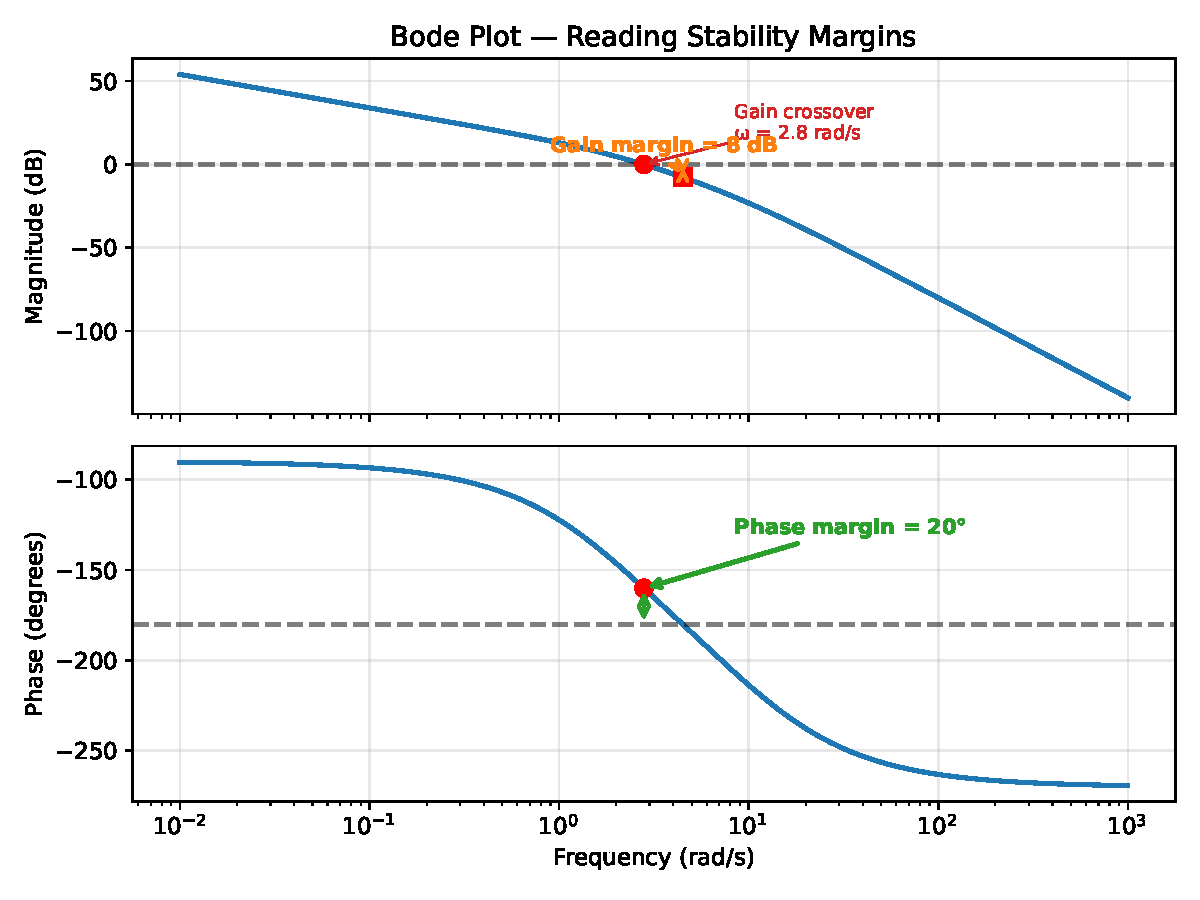
\includegraphics[width=\textwidth]{bode_plot.pdf}
\caption{开环系统 $L(s) = \frac{100}{s(s+2)(s+10)}$ 的Bode图。增益裕度（橙色）和相位裕度（绿色）可直接从图中读取。两者均为正值，故系统稳定。}
\end{figure}

\textbf{经验法则：}如果系统振荡，说明相位裕度太小。如果系统响应迟钝，说明增益裕度太大（你过于保守了）。相位裕度约45°通常能取得不错的平衡。

\subsection{基于传递函数的控制器设计}

我们已经学会了从 Bode 图上读出稳定裕度——换句话说，我们能诊断问题了。接下来自然要问：怎么治？

经典控制器设计的目标是：给定被控对象 $G(s)$，选择控制器 $C(s)$，使得闭环系统 $\frac{C(s)G(s)}{1+C(s)G(s)}$ 满足性能指标。

方法有很多——根轨迹（一种图形方法，画出增大控制器增益时系统极点在复平面上的移动轨迹）、频率响应整形（通过调整 Bode 图形状来满足指标）、极点配置（直接选择闭环极点应该放在哪里）——但对于竞赛机器人而言，最实用的方法是：

\begin{enumerate}
    \item 从PID控制器出发（下一节介绍）。
    \item 用系统化的方法进行整定。
    \item 如果PID不够，添加前馈或切换到现代方法（第6节）。
\end{enumerate}

听起来好像不够高大上？事实就是：全世界大约 95\% 的工业控制回路跑的都是 PID。简单、皮实、管用。没必要把事情搞复杂。

\subsection{PID控制器}

PID 控制器把误差 $e(t)$ 拆成三项来计算控制信号：

\begin{equation}
u(t) = K_p e(t) + K_i \int_0^t e(\tau) d\tau + K_d \frac{de(t)}{dt}
\end{equation}

三项各司其职：

\begin{itemize}
    \item \textbf{P（比例）：}"差多少就推多少"——误差大就猛推，误差小就轻推。最直觉的一项，像弹簧。
    \item \textbf{I（积分）：}"这误差怎么老不消？肯定有东西在拖后腿。"它一直攒力气直到误差归零。能消稳态误差，但容易超调和积分饱和（windup）。
    \item \textbf{D（微分）：}"误差在猛变，赶紧踩刹车！"它提供阻尼、压制超调，但也会放大噪声。
\end{itemize}

\textbf{打个比方：}你开车，前面有个停车标志。
\begin{itemize}
    \item P："还有 100 米，踩油门。""还有 10 米，松油门。"
    \item D："靠近得太快了——现在就刹车，别等到跟前！"
    \item I："停在标志前 1 米了，没对准。慢慢蹭，蹭到精确位置。"
\end{itemize}

\subsubsection{PID控制器——连续形式}

直觉建立起来了，现在我们需要频域的语言——因为接下来分析滤波器、导数噪声放大、Bode 整形全都要用到它。

PID控制器的传递函数为：
\begin{equation}
C(s) = K_p + \frac{K_i}{s} + K_d s = K_p \left(1 + \frac{1}{T_i s} + T_d s\right)
\end{equation}

其中 $T_i = K_p / K_i$ 是积分时间，$T_d = K_d / K_p$ 是微分时间。

\textbf{从频域理解PID：}

PID控制器的Bode图揭示了它为何有效：
\begin{itemize}
    \item \textbf{极低频处}（$\omega \to 0$）：$K_i/s$ 项主导。增益趋向无穷大（$+\infty$ dB），I 项之所以能消稳态误差，就是因为这一点——直流处增益无穷大，直流误差必须为零。
    \item \textbf{中频处}：$K_p$ 主导。增益约为 $20\log_{10}(K_p)$ dB。控制器的大部分工作在这个频率范围完成。
    \item \textbf{高频处}（$\omega \to \infty$）：$K_d s$ 主导。增益以 $+20$ dB/decade 随频率增大，D 项放大噪声的原因就在这里——噪声的频率越高，D 项的增益越大。
\end{itemize}

PID有\textbf{两个折断频率（break frequencies）}：$\omega_1 = 1/T_i$（I项移交给P项）和 $\omega_2 = 1/T_d$（P项移交给D项）。两者之间，控制器表现为纯比例控制。幅频图在对数坐标下看起来像"V"形（或浴缸形）：低频处增益大（I），中间平坦（P），高频处上升（D）。

\textbf{为什么另一种形式很重要：}$K_p(1 + \frac{1}{T_i s} + T_d s)$ 的形式使物理含义更清晰：$T_i$ 表示"积分项回看多久"，$T_d$ 表示"微分项向前预测多远"。$T_i$ 越大，积分动作越慢。$T_d$ 越大，预测性越强（但对噪声也更敏感）。

\textbf{各增益的影响：}

\begin{center}
\begin{tabular}{lcccc}
\toprule
\textbf{增大} & \textbf{上升时间} & \textbf{超调量} & \textbf{调节时间} & \textbf{稳态误差} \\
\midrule
$K_p$ & 减小 & 增大 & 小幅变化 & 减小 \\
$K_i$ & 减小 & 增大 & 增大 & 消除 \\
$K_d$ & 小幅变化 & 减小 & 减小 & 无影响 \\
\bottomrule
\end{tabular}
\end{center}

\textbf{调参起手式：}先只用 P。有稳态误差？加 I。超调或振荡太大？加 D。千万别三个参数同时非零地往上调——你根本分不清是哪个旋钮在起作用。

\vspace{0.5em}
\begin{mdframed}[linewidth=1pt, innertopmargin=10pt, innerbottommargin=10pt]
\textbf{案例分析：整定云台偏航电机——亲眼看P、I、D各自的作用}

\vspace{0.3em}
下面一步步整定 RoboMaster 云台偏航轴。电机 GM6020，CAN 总线控制，目标是跟踪角度。设定值：90° 阶跃。

\textbf{第1步：只用P（$K_p = 5.0$，$K_i = 0$，$K_d = 0$）}

云台快速向目标摆动，但超调约15°，振荡3--4次，最终以\textbf{2°的稳态误差}稳定。为什么有误差？因为云台接近目标时，误差变小，P项输出也随之减小。到某个时刻，P项输出等于摩擦力矩，云台在\textit{还未到达}目标时就停下来了。单靠P项无法消除持续扰动（如摩擦或重力）引起的误差。

\textbf{第2步：加入I（$K_p = 5.0$，$K_i = 0.5$，$K_d = 0$）}

稳态误差消失了！积分项缓慢积累小的残余误差并推动电机，直到误差精确为零。但现在超调更大了（约20°），还有缓慢振荡，需要2秒才能衰减。积分项在"记住"过去的误差并施加了不必要的力。这是I项经典的权衡：修复了直流误差，但使瞬态响应变差了。

\textbf{第3步：加入D（$K_p = 5.0$，$K_i = 0.5$，$K_d = 2.0$）}

超调量大幅下降至约5°，振荡几乎消失。微分项感知到快速靠近并在云台到达目标\textit{之前}施加制动力矩。就像一位经验丰富的司机，在到达路口前很早就开始刹车，而不是到最后一刻。

\textbf{第4步：精细调整（$K_p = 6.0$，$K_i = 0.3$，$K_d = 3.0$）}

略微增大 $K_p$ 以加快上升速度，减小 $K_i$（我们只需要它来克服静摩擦，不需要激进的误差纠正），增大 $K_d$ 以增加阻尼。结果：快速、平滑的跟踪，超调不到3°，稳态误差为零。云台在0.3秒内锁定目标。

\textbf{把每个参数调到过大会发生什么？}
\begin{itemize}[nosep]
    \item $K_p$ 过大：云台剧烈振荡——超调太猛，纠正动作又向另一方向超调。这是失稳的前兆。
    \item $K_i$ 过大：缓慢、黏糊的振荡。积分"记得"太用力，不断过度纠正。云台像果冻一样摇摆。
    \item $K_d$ 过大：电机嗡嗡震动。微分放大传感器噪声，导致快速来回的力矩指令。你的电机听起来像一只愤怒的蜜蜂。
\end{itemize}

\textbf{教训：}每个参数都有一个"甜蜜点"。搞懂每一项的\textit{物理机制}（弹簧、记忆、阻尼器），出了问题你就能秒定位，而不是蒙着眼乱拧旋钮。
\end{mdframed}

\begin{figure}[H]
\centering
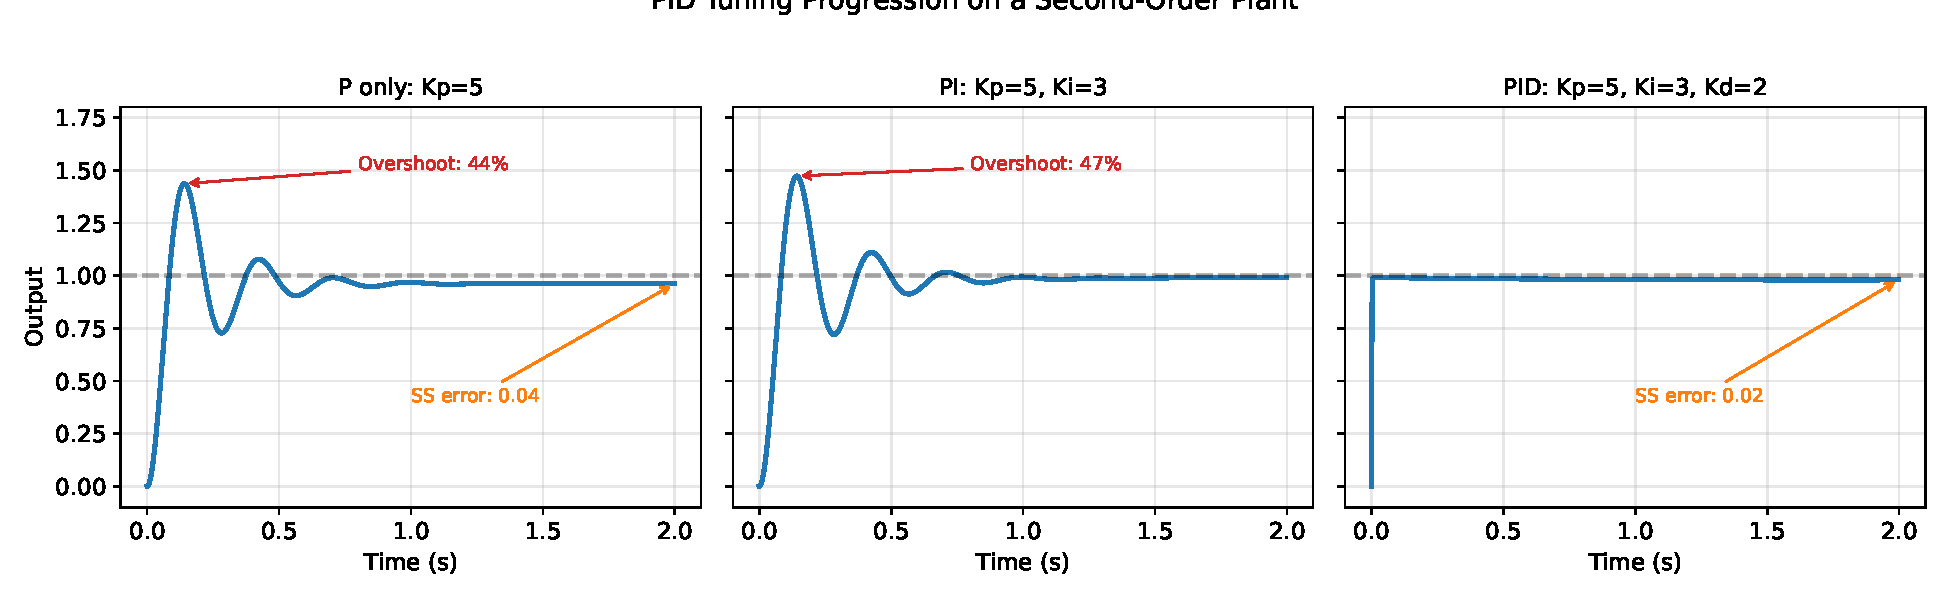
\includegraphics[width=\textwidth]{pid_tuning.pdf}
\caption{二阶被控对象上的PID整定过程。纯P存在稳态误差；PI消除稳态误差但超调更大；PID在保持零稳态误差的同时抑制了超调。}
\end{figure}

\subsubsection{PID控制器——离散形式}

你的微控制器无法计算连续的积分和微分，它以固定采样时间步长 $T_s$ 处理离散样本。离散PID为：

\begin{equation}
u[n] = K_p \, e[n] + K_i \, T_s \sum_{k=0}^{n} e[k] + K_d \frac{e[n] - e[n-1]}{T_s}
\end{equation}

或者用更便于实现的\textbf{增量式（速度式）形式（incremental / velocity form）}：
\begin{equation}
\Delta u[n] = K_p (e[n] - e[n-1]) + K_i \, T_s \, e[n] + K_d \frac{e[n] - 2e[n-1] + e[n-2]}{T_s}
\end{equation}

\begin{equation}
u[n] = u[n-1] + \Delta u[n]
\end{equation}

增量式的实践优势：如果控制器复位或出现故障，不会突然产生大幅输出——每次只调整一个小增量。这对你的硬件更安全。

\textbf{基础离散PID伪代码：}
\begin{verbatim}
    error = setpoint - measurement
    integral += error * dt
    derivative = (error - prev_error) / dt
    output = Kp * error + Ki * integral + Kd * derivative
    prev_error = error
\end{verbatim}

\textbf{警告：}这种朴素实现在实践中有三个问题会坑到你：积分饱和（integral windup）、微分冲击（derivative kick）和噪声放大。请阅读下一节。

\subsubsection{改进的PID控制器}

你照着教科书写了一个标准 PID，上传代码，电机开始跑——然后积分项越来越大，输出饱和了，松开设定值后电机猛地甩过头。为什么？因为教科书的 PID 有几个众所周知的坑，每个竞赛机器人都必须补上。

这些问题并非彼此独立——饱和、冲击和噪声放大都源于同一根源：PID 的三个项在执行器极限或高频处表现不佳。

\textbf{1. 积分饱和与抗积分饱和（Integral Windup and Anti-windup）}

\textit{问题：}执行器饱和了（电机已经到最大电压），积分项还在拼命攒误差。等误差方向反过来，积分值已经攒得巨大，要很久才能"退饱和"，于是大幅超调。

\textit{修复方案（限幅法）：}
\begin{verbatim}
    integral += error * dt
    integral = clamp(integral, -max_integral, max_integral)
\end{verbatim}

\textit{更好的修复方案（反向计算法）：}当输出饱和时，按比例减小积分项：
\begin{verbatim}
    output_raw = Kp * error + Ki * integral + Kd * derivative
    output = clamp(output_raw, -max_output, max_output)
    integral += (error + (output - output_raw) / Ki) * dt
\end{verbatim}

驯服了积分之后，下一个隐患出现在设定值突变时。

\textbf{2. 微分冲击（Derivative Kick）}

\textit{问题：}设定值突变（阶跃指令），误差 $e = r - y$ 瞬间跳一大截。微分项把它当成无限大的变化率，输出直接飙出一个巨大尖峰。

\textit{修复方案：}对\textit{测量值}求导，而非对误差求导：
\begin{verbatim}
    derivative = -(measurement - prev_measurement) / dt
\end{verbatim}

测量值变化是平滑的（电机又不会瞬移），自然不会有冲击。

对测量值求导而非误差解决了冲击问题，但引入了一个更隐蔽的问题。

\textbf{3. 微分噪声放大（Derivative Noise Amplification）}

\textit{问题：}微分放大高频噪声。测量值一有噪声，微分项的输出就剧烈抖动。

\textit{修复方案：}对微分项进行低通滤波：
\begin{equation}
D(s) = \frac{K_d s}{1 + \frac{K_d}{N K_p} s}
\end{equation}

在代码中，这是对微分项的一阶低通滤波，$N$（通常为8--20）控制滤波器截止频率。

前三个修复让 PID 变得鲁棒，最后一个让它变得灵活。

\textbf{4. 设定值加权（Setpoint Weighting）}

有时你希望P项和D项对设定值变化与扰动的响应不同。设定值加权引入参数 $b$ 和 $c$：
\begin{equation}
u = K_p(b \cdot r - y) + K_i \int (r - y) \, dt + K_d \frac{d(c \cdot r - y)}{dt}
\end{equation}

设 $b = 1, c = 0$（仅对测量值求导）是最常见的配置。

\subsection{PID进阶改进}

以上四个修复是竞赛机器人的\textit{底线}。但还有更深一层的结构性改进，能让性能产生质的变化。下面从频域角度分析，配合仿真演示。

\subsubsection{积分分离（Integral Separation）}

\textit{问题：}当误差较大时（例如刚收到阶跃指令后），积分项积极累积。这个"预充电"的积分在系统接近设定值时会引起超调——积分"记住"了大误差阶段太多的历史。

\textit{修复方案：}只有当误差小于阈值 $\varepsilon$ 时才激活积分项：
\begin{equation}
u_I = \begin{cases} K_i \int e \, dt & \text{如果 } |e| < \varepsilon \\ 0 & \text{如果 } |e| \geq \varepsilon \end{cases}
\end{equation}

\textbf{频域解释：}积分分离实际上使控制器变成\textbf{非线性}——大误差时表现为PD控制器（无积分），小误差时切换为完整的PID。在频域中，这意味着：
\begin{itemize}
    \item 大瞬态期间：直流处的开环增益是有限的（仅PD），因此不存在无穷低频增益。这防止了积分在瞬态期间的"饱和"。
    \item 接近稳态时：积分激活，提供无穷直流增益和零稳态误差——正是我们需要的。
\end{itemize}

控制器实际上根据误差幅度拥有\textbf{两种不同的Bode图}：一种没有低频处的 $K_i/s$ 极点（类PD），一种有（PID）。阈值 $\varepsilon$ 控制"切换"的时机。

\textbf{代码：}
\begin{verbatim}
    if (fabs(error) < epsilon) {
        integral += Ki * error * dt;
    }
    // 否则：积分保持冻结（既不增长也不复位）
\end{verbatim}

\textbf{如何选择 $\varepsilon$：}将其设置为纯PD控制器的近似稳态误差。这样，积分仅在PD完成了大部分工作、只需要最后一点"微调"时才激活。

\begin{figure}[H]
\centering
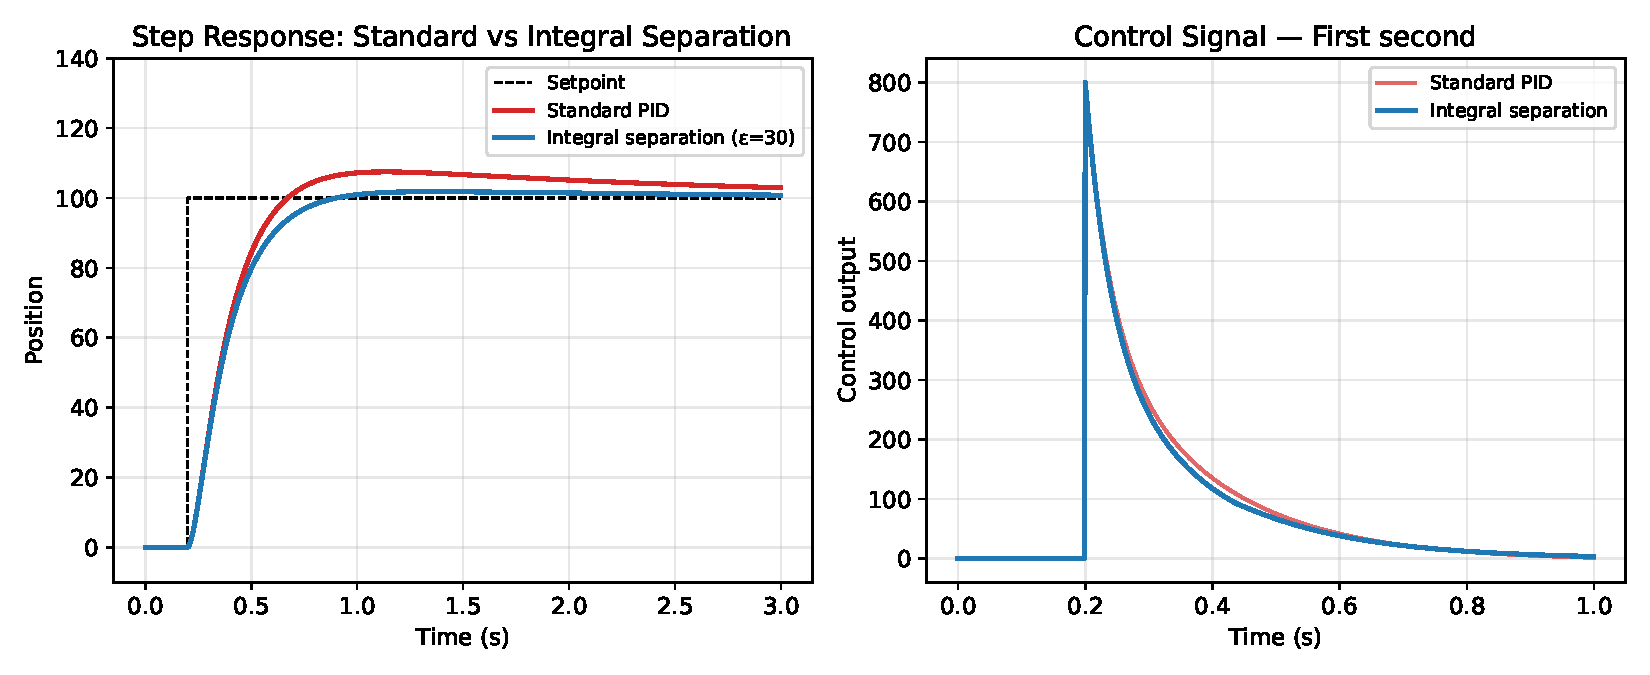
\includegraphics[width=\textwidth]{integral_separation.pdf}
\caption{左图：积分分离（蓝色）相比标准PID（红色）减少了超调，因为积分不在大初始瞬态期间累积。右图：第一秒内的控制信号——注意分离版本的峰值更小。}
\end{figure}

\subsubsection{微分位置：PID vs PI-D vs I-PD}

标准PID将三项都作用于误差 $e = r - y$。但有\textbf{三种结构变体}，改变了P项和D项作用于哪个信号：

\begin{center}
\begin{tabular}{lccc}
\toprule
\textbf{结构} & \textbf{P作用于} & \textbf{I作用于} & \textbf{D作用于} \\
\midrule
PID & 误差 $(r - y)$ & 误差 $(r - y)$ & 误差 $(r - y)$ \\
PI-D & 误差 $(r - y)$ & 误差 $(r - y)$ & 测量值 $(-y)$ \\
I-PD & 测量值 $(-y)$ & 误差 $(r - y)$ & 测量值 $(-y)$ \\
\bottomrule
\end{tabular}
\end{center}

\textbf{频域分析：}三种结构具有\textit{相同的}闭环抗扰传递函数（从扰动到输出）。它们仅在\textit{设定值到输出}的传递函数上有所不同：

\begin{itemize}
    \item \textbf{PID：}$\frac{Y}{R} = \frac{(K_d s^2 + K_p s + K_i) G(s)}{s + (K_d s^2 + K_p s + K_i) G(s)}$ ——分子含 $K_d s^2$ 项，在阶跃响应中产生"微分冲击"（分子零点放大了阶跃的高频成分）。
    \item \textbf{PI-D：}$\frac{Y}{R} = \frac{(K_p s + K_i) G(s)}{s + (K_d s^2 + K_p s + K_i) G(s)}$ ——从设定值通路中移除了 $K_d s^2$，消除了微分冲击。分母（稳定性、抗扰性）不变。
    \item \textbf{I-PD：}$\frac{Y}{R} = \frac{K_i \cdot G(s)}{s + (K_d s^2 + K_p s + K_i) G(s)}$ ——从设定值通路中同时移除 $K_d s^2$ 和 $K_p s$。阶跃响应最平滑（无P或D引起的超调），但也最慢。
\end{itemize}

\textbf{要点：}这些结构让你可以把\textit{设定值跟踪}（分子控制）和\textit{抗扰性能}（分母控制）拆开来分别调。分母一样 = 稳定性和抗扰性一样；分子不同 = 设定值跟踪行为不同。

\begin{figure}[H]
\centering
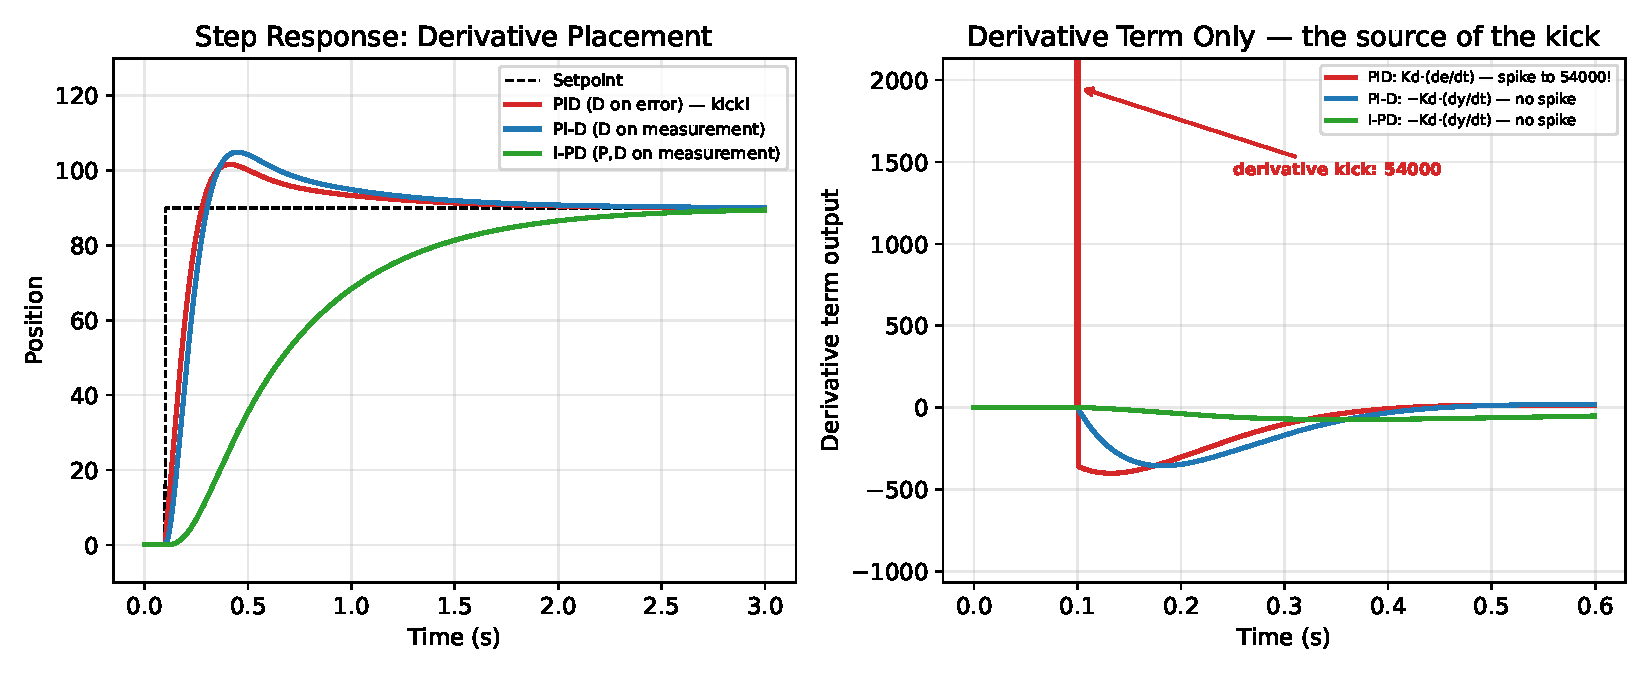
\includegraphics[width=\textwidth]{derivative_placement.pdf}
\caption{左图：PID（红色）显示微分冲击尖峰和超调。PI-D（蓝色）消除了冲击。I-PD（绿色）最平滑但最慢。右图：控制信号揭示了标准PID中的剧烈冲击——这个尖峰会磨坏齿轮。}
\end{figure}

\subsubsection{滤波PID：频域证明}

理想PID控制器 $C(s) = K_p + K_i/s + K_d s$ 有一个根本性问题：$K_d s$ 项在高频处具有\textbf{无界增益}。在Bode图上，$K_d s$ 的幅值以 $+20$ dB/decade 永远上升。这意味着：

\begin{enumerate}
    \item 传感器噪声（存在于高频）被无限放大。
    \item 控制器要求执行器响应速度无限快，这在物理上是不可能的。
    \item 在离散时间中，微分项将高频噪声混叠进控制带。
\end{enumerate}

\textbf{解决方案——滤波微分（filtered derivative）：}
\begin{equation}
C_{\text{filtered}}(s) = K_p + \frac{K_i}{s} + \frac{K_d N s}{s + N}
\end{equation}

$\frac{Ns}{s+N}$ 项是截止频率为 $\omega = N$ rad/s 的一阶高通滤波器。在 $N$ 以下，它表现为纯微分（$\approx s$）。在 $N$ 以上，它趋于常数增益 $N$。在Bode图上：

\begin{itemize}
    \item $\omega < N$ 处：滤波PID与理想PID完全相同，性能一致。
    \item $\omega > N$ 处：幅值\textbf{趋于平坦}，而不是永远上升。最大微分增益为 $K_d \cdot N$，噪声放大有界。
\end{itemize}

\textbf{如何选择 $N$：}典型值为 $N = 8$--$20$。规则：$N$ 要足够大，使微分在控制器带宽处仍有效工作；但也要足够小以衰减噪声。具体而言：$N > 5 \times \omega_{\text{bandwidth}}$（避免滤波器吃掉有用的微分作用）且 $N < \omega_{\text{noise}} / 3$（充分衰减噪声）。

\begin{figure}[H]
\centering
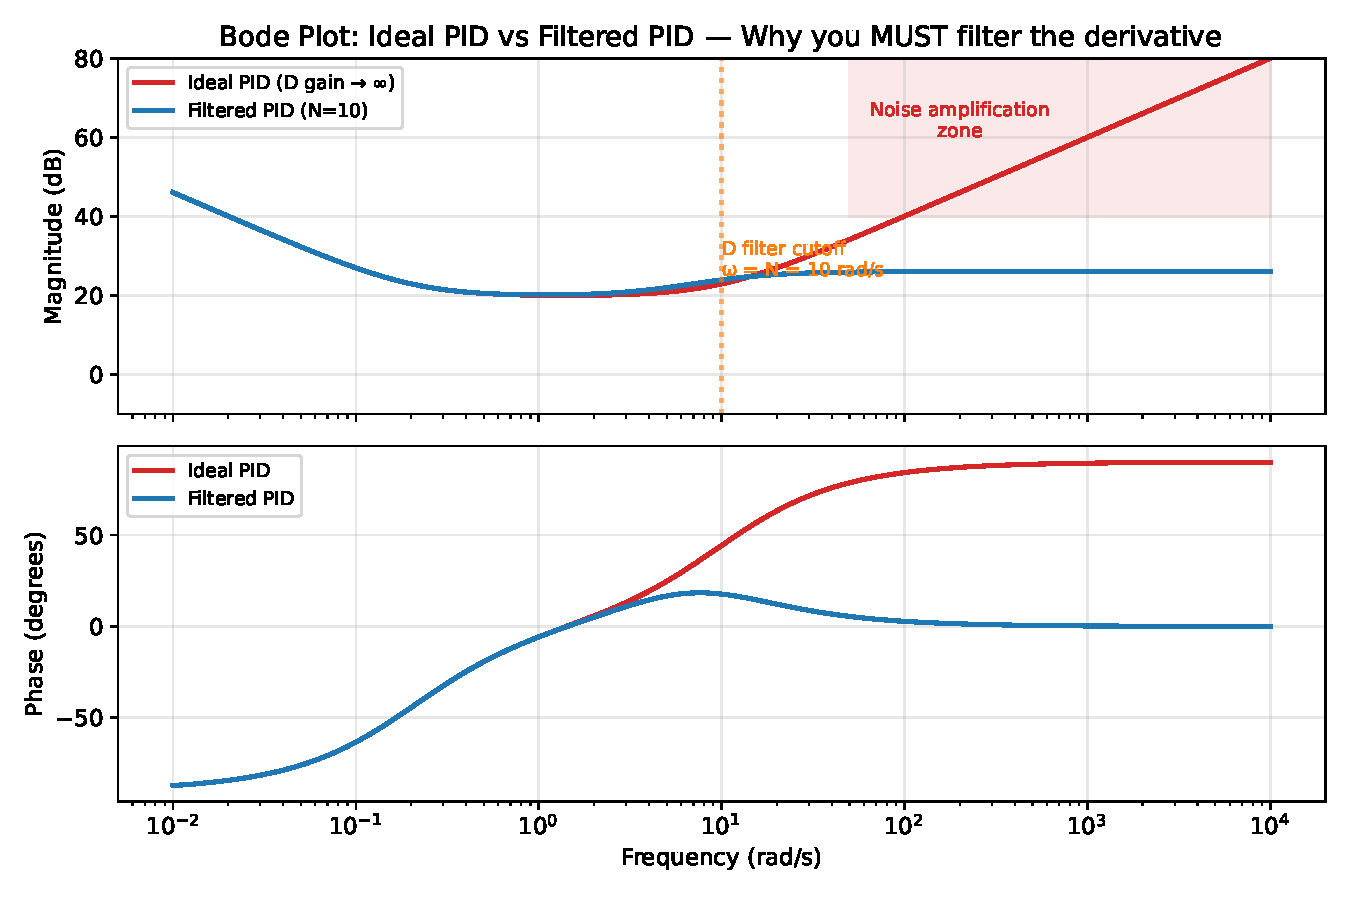
\includegraphics[width=\textwidth]{pid_bode_comparison.pdf}
\caption{Bode图：理想PID（红色）在高频处增益永远上升——它会放大每一点传感器噪声。滤波PID（蓝色）在 $\omega = N$ 以上趋于平坦，限制了噪声放大。在滤波器截止频率以下，两者完全相同。}
\end{figure}

\textbf{输出级低通滤波器（Output-stage LPF）：}另一种方法是在将PID输出发送到执行器前，对\textit{整个}PID输出进行低通滤波：
\begin{equation}
U(s) = \frac{\omega_f}{s + \omega_f} \cdot C(s) \cdot E(s)
\end{equation}

这种方法实现更简单（PID后加一个低通滤波器），但它同时滤掉了P项和I项，可能减慢响应速度。仅对微分项滤波的方案更受青睐，因为它精确地针对问题所在。

\begin{figure}[H]
\centering
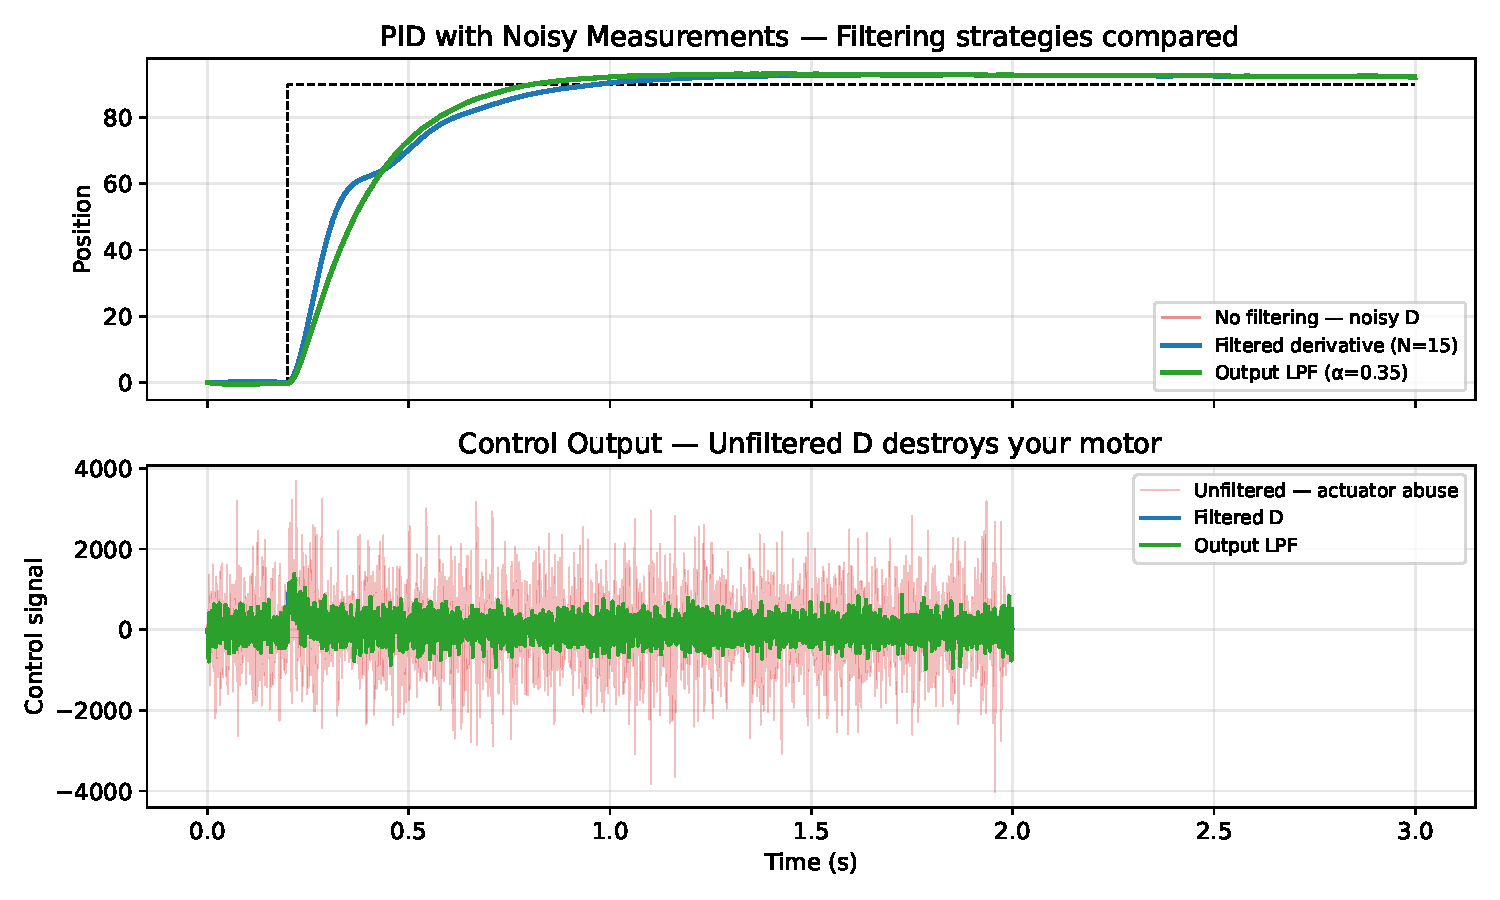
\includegraphics[width=\textwidth]{pid_noise_filtering.pdf}
\caption{上图：带噪声测量的位置响应。未滤波PID（红色）因噪声放大的微分项而振荡。滤波微分（蓝色）和输出低通滤波（绿色）都能平滑响应。下图：未滤波的控制信号非常剧烈——会损坏真实的电机。}
\end{figure}

\subsubsection{二自由度PID（2-DOF PID）}

标准PID有\textbf{一个自由度}：你选择 $K_p$、$K_i$、$K_d$ 来满足你的指标。但存在一个根本性冲突：能给出良好\textit{设定值跟踪}（快速、低超调的阶跃响应）的增益，与能给出良好\textit{抗扰性}（受扰后快速恢复）的增益不同。

二自由度PID通过引入设定值加权参数 $b$（作用于P项）和 $c$（作用于D项）来解决这一矛盾：
\begin{equation}
u = K_p(b \cdot r - y) + K_i \int (r - y) \, dt + K_d \frac{d(c \cdot r - y)}{dt}
\end{equation}

\textbf{频域分析：}闭环传递函数变为：
\begin{align}
\frac{Y}{R} &= \frac{(b K_p + c K_d s + K_i / s) \cdot G(s)}{1 + C(s) G(s)} \quad \text{（设定值跟踪——由 $b$、$c$ 调节）} \\[4pt]
\frac{Y}{D} &= \frac{G(s)}{1 + C(s) G(s)} \quad \text{（抗扰性——与 $b$、$c$ 无关！）}
\end{align}

\textbf{神奇之处：}$b$ 和 $c$ \textit{只}影响设定值传递函数。抗扰性完全由 $K_p$、$K_i$、$K_d$ 控制。现在你可以：
\begin{enumerate}
    \item 调整 $K_p$、$K_i$、$K_d$ 以实现激进的抗扰性。
    \item 独立地降低 $b$（通常为 $0.5$--$0.8$）来柔化设定值响应并减少超调。
    \item 设 $c = 0$ 以消除微分冲击（这就是PI-D结构）。
\end{enumerate}

\begin{figure}[H]
\centering
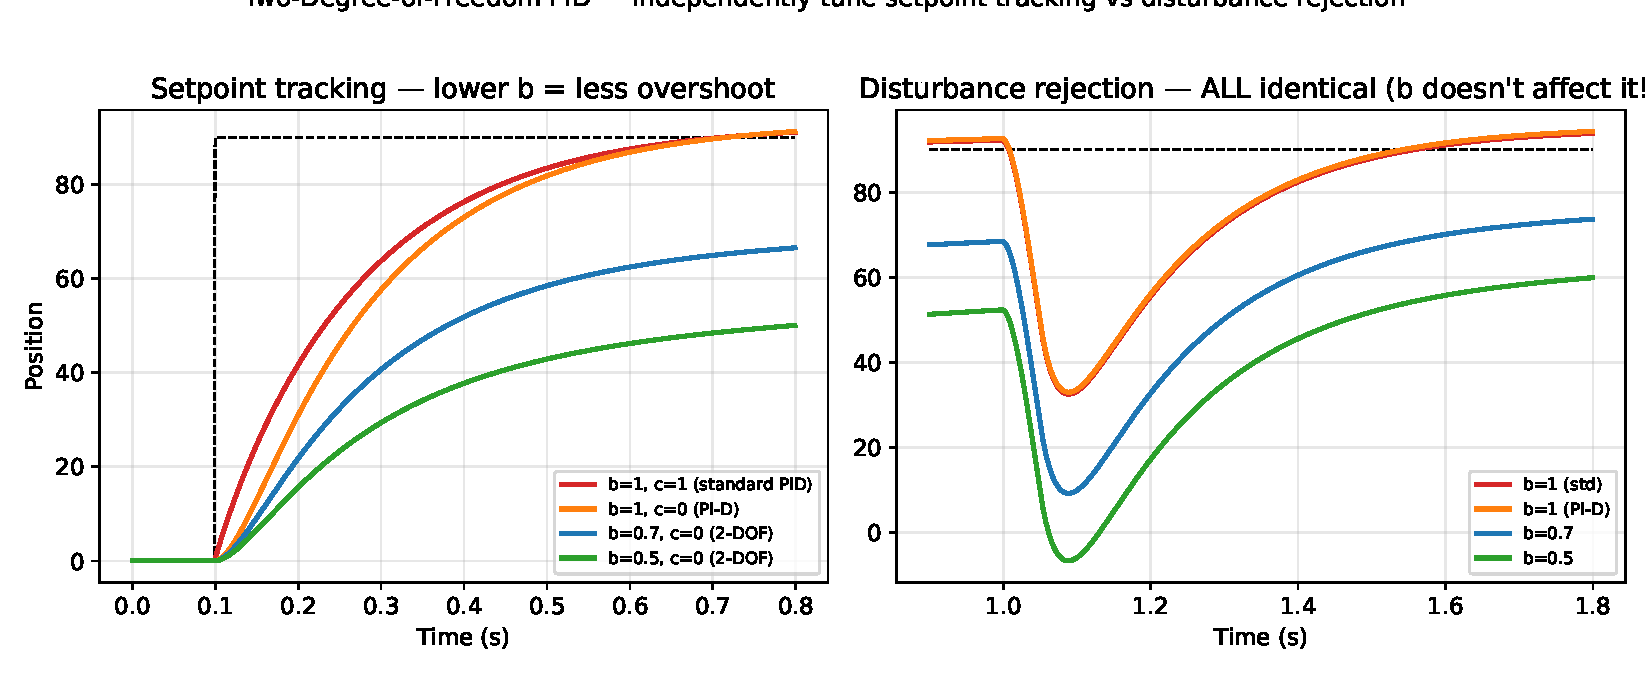
\includegraphics[width=\textwidth]{two_dof_pid.pdf}
\caption{左图：不同的 $b$ 值独立控制设定值超调。右图：$t = 1.0$s 时的扰动抑制对所有 $b$ 值\textbf{完全相同}——证明了二自由度PID真正实现了两个目标的解耦。}
\end{figure}

\subsubsection{模糊PID（Fuzzy PID）}

\textbf{动机。}标准PID控制器使用固定增益 $K_p$、$K_i$、$K_d$。然而\emph{最优}增益取决于工作状态：误差较大时需要激进的响应，误差较小时则需要精细控制。模糊PID根据当前误差 $e$ 及其变化率 $\dot{e}$ 实时调整 $K_p$、$K_i$、$K_d$。

\textbf{工作原理。}
\begin{enumerate}
    \item \textbf{模糊化（Fuzzification）。}为误差 $e$ 及其导数 $\dot{e}$ 定义模糊集合。常用的划分包含五个语言变量：NB（负大）、NS（负小）、ZO（零）、PS（正小）、PB（正大）。隶属度函数（通常为三角形或梯形）将 $e$ 和 $\dot{e}$ 的精确值映射为各模糊集合的隶属度。
    \item \textbf{规则表。}一张规则表（例如 $5 \times 5$ 或 $7 \times 7$）将 $(e,\, \dot{e})$ 的每种组合映射为增益调整量 $(\Delta K_p,\, \Delta K_i,\, \Delta K_d)$。规则以自然语言描述，例如：
    \begin{itemize}
        \item ``若 $e$ 为PB且 $\dot{e}$ 为PB $\Rightarrow$ 大幅增大 $K_p$，减小 $K_i$（防止积分饱和），增大 $K_d$。''
        \item ``若 $e$ 为ZO且 $\dot{e}$ 为NS $\Rightarrow$ 保持 $K_p$ 适中，启用 $K_i$ 以消除稳态误差，减小 $K_d$。''
    \end{itemize}
    \item \textbf{解模糊（Defuzzification）。}将触发的规则进行聚合（常用重心法），得到 $\Delta K_p$、$\Delta K_i$、$\Delta K_d$ 的精确值。
    \item \textbf{增益更新。}实际PID增益为：
    \[
        K_p = K_{p0} + \Delta K_p, \qquad K_i = K_{i0} + \Delta K_i, \qquad K_d = K_{d0} + \Delta K_d
    \]
    其中 $K_{p0}$、$K_{i0}$、$K_{d0}$ 为基准增益。
\end{enumerate}

\textbf{$\Delta K_p$ 简化规则表示例（$3 \times 3$）。}
\begin{center}
\begin{tabular}{c|ccc}
    $e$ \textbackslash{} $\dot{e}$ & N & Z & P \\
    \hline
    N & PB & PS & ZO \\
    Z & PS & ZO & NS \\
    P & ZO & NS & NB \\
\end{tabular}
\end{center}
解读：当误差为负且持续增大（$\dot{e} = $ N）时，大幅增加 $K_p$（PB）以驱动系统回到目标；当两者均接近零时，无需调整（ZO）。

\textbf{实践评估。}
\begin{itemize}
    \item \textbf{优势：}模糊PID能够适应变化的工况——负载变化、非线性工作区域——而无需显式系统模型。
    \item \textbf{不足：}规则表的设计主要依赖经验。实质上是将``整定3个增益''转化为``整定一张规则表''，且更难以严格验证。
    \item \textbf{适用场景：}在竞赛机器人中，精心整定的固定PID或二自由度PID通常已经足够。当系统需要在差异显著的工况间切换时（例如底盘需同时适应空载和满载状态），模糊PID值得考虑。
    \item \textbf{与增益调度的对比：}增益调度在离散工作点之间手动切换预整定的PID参数集，切换边界处可能产生暂态。模糊PID由于隶属度函数在规则之间自然插值，能够提供更平滑的过渡。
\end{itemize}

\subsection{PID整定方法}

你已经设计好了PID控制器。现在来回答那个永恒的问题：$K_p$、$K_i$、$K_d$ 应该取什么值？

\subsubsection{经验整定}

比赛中最常用的方法，因为不需要数学推导，效果却出人意料地好。

\textbf{Ziegler-Nichols极限增益法（ultimate gain method）：}
\begin{enumerate}
    \item 令 $K_i = 0$，$K_d = 0$。
    \item 逐渐增大 $K_p$，直到系统以恒定幅值振荡。此时的 $K_p$ 即为\textbf{极限增益（ultimate gain）} $K_u$，振荡周期为 $T_u$。
    \item 按下表设置PID增益：
\end{enumerate}

\begin{center}
\begin{tabular}{lccc}
\toprule
\textbf{控制器} & $K_p$ & $K_i$ & $K_d$ \\
\midrule
P & $0.5 K_u$ & --- & --- \\
PI & $0.45 K_u$ & $0.54 K_u / T_u$ & --- \\
PID & $0.6 K_u$ & $1.2 K_u / T_u$ & $0.075 K_u T_u$ \\
\bottomrule
\end{tabular}
\end{center}

\textbf{警告：}Ziegler-Nichols给出的整定结果比较激进，超调量约25\%。对于许多竞赛应用，你需要在此基础上适当减小 $K_p$ 和 $K_i$。

\textbf{手动整定（实用方法）：}
\begin{enumerate}
    \item 先只用 $K_p$。增大到响应快但略有振荡。
    \item 加入 $K_d$ 以抑制振荡。增大到振荡消失。
    \item 如果有稳态误差，加入少量 $K_i$。缓慢增大——过大会引起缓慢振荡。
    \item 精细调整。用不同设定值和扰动进行测试。
\end{enumerate}

\textbf{竞赛建议：}始终在机器人\textit{实际负载}下整定，而不是让电机空转。装了摄像头的云台与裸电机在测试台上的表现差异悬殊。

\subsubsection{使用MATLAB Simulink整定}

如果你能用MATLAB，可以对系统建模，并使用\textbf{PID整定器（PID Tuner）}应用程序或\textbf{Simulink Control Design}自动找到最优增益。

\textbf{基本流程：}
\begin{enumerate}
    \item 在Simulink中建立被控对象模型（电机 + 负载）。
    \item 添加PID控制器模块。
    \item 在PID模块中点击"Tune"按钮，打开PID整定器。
    \item 调整响应时间和鲁棒性滑块。
    \item 将增益导出到你的嵌入式代码中。
\end{enumerate}

在硬件上精调之前拿到一个起始点，很好用。但前提是被控对象模型得准——模型错了，整定出来的参数也是错的。

\subsection{系统辨识：搞清楚你的被控对象究竟如何工作}

到目前为止，我们假设你\textit{知道}被控对象模型——传递函数 $G(s)$ 或状态空间矩阵 $A$、$B$、$C$、$D$。但这些从哪里来？你有两个选择：

\begin{enumerate}
    \item \textbf{第一性原理建模（First-principles Modeling）：}写出物理方程（牛顿定律、基尔霍夫定律等），解析推导模型。第 3 节里对直流有刷电机做的就是这个。物理过程简单、理解充分的时候效果最好。
    \item \textbf{系统辨识（System Identification，Sysid）：}向真实系统施加已知输入，测量输出，然后\textit{拟合}数学模型到输入-输出数据。当物理过程过于复杂、未知，或者你想捕捉第一性原理模型忽略的效应（非线性摩擦、缆线刚度、齿轮间隙）时使用。
\end{enumerate}

实际做的时候，几乎总是\textbf{两手都用}：第一性原理定结构（"这是一个带延迟的二阶系统"），系统辨识定参数（$K$、$\tau$、$\zeta$ 等）。

\subsubsection{阶跃响应法（时域）}

最简单的系统辨识技术。施加阶跃输入并记录输出。

\textbf{对于一阶系统} $G(s) = \frac{K}{\tau s + 1}$：
\begin{enumerate}
    \item 向电机电压施加幅值为 $A$ 的阶跃。
    \item 记录速度响应 $y(t)$。
    \item 读取：
    \begin{itemize}[nosep]
        \item $K$ = （最终稳态值）/ $A$ = 直流增益
        \item $\tau$ = 到达终值63.2\%所需的时间 = 时间常数
    \end{itemize}
\end{enumerate}

\textbf{对于二阶系统} $G(s) = \frac{K\omega_n^2}{s^2 + 2\zeta\omega_n s + \omega_n^2}$：
\begin{enumerate}
    \item 施加阶跃并记录。
    \item 读取：
    \begin{itemize}[nosep]
        \item $K$ = （终值）/（阶跃幅值）
        \item $M_p$ = 百分比超调量 $\Rightarrow$ $\zeta = \frac{-\ln(M_p/100)}{\sqrt{\pi^2 + \ln^2(M_p/100)}}$

        由超调公式 $M_p = e^{-\pi\zeta/\sqrt{1-\zeta^2}}$ 两边取对数得 $\ln(M_p/100) = -\pi\zeta/\sqrt{1-\zeta^2}$，平方两边并解出 $\zeta$ 即得。
        \item $t_p$ = 第一个峰值出现的时间 $\Rightarrow$ $\omega_n = \frac{\pi}{t_p \sqrt{1 - \zeta^2}}$
    \end{itemize}
\end{enumerate}

\textbf{实践建议：}
\begin{itemize}
    \item 以传感器支持的最高速率记录数据（电机1 kHz以上）。
    \item 测试运行3--5次取平均以减小噪声影响。
    \item 用不同阶跃幅值测试以检验线性性。若响应形状改变，系统是非线性的。
    \item 同时记录上升阶跃（0 $\to$ V）和下降阶跃（V $\to$ 0）。若两者不同，说明存在不对称动态（如正反转摩擦不同）。
\end{itemize}

\subsubsection{频率响应法（Bode辨识）}

在不同频率施加正弦输入，在每个频率测量增益和相移。这直接构造出系统的Bode图。

\textbf{步骤：}
\begin{enumerate}
    \item 向系统施加 $u(t) = A \sin(\omega t)$。
    \item 等待瞬态消失（几个周期）。
    \item 测量稳态输出幅值 $B$ 和相位滞后 $\phi$。
    \item 计算增益：$|G(j\omega)| = B/A$，相位：$\angle G(j\omega) = \phi$。
    \item 在期望带宽的0.1$\times$至10$\times$范围内重复上述步骤。
\end{enumerate}

\textbf{这方法的厉害之处：}Bode 图能直接告诉你系统阶次（数斜率变化的段数）、共振频率（幅值图上的峰）和时间延迟（相位线性下降）。有了 Bode 图就可以拟合传递函数。

\textbf{更快的替代——扫频信号（Chirp）：}一个个频率挨个测太慢了。直接给一个\textbf{chirp}——频率在几秒内从低扫到高。然后对输入输出分别做 FFT，一除：$G(j\omega) = \frac{Y(j\omega)}{U(j\omega)}$。一次实验拿到完整 Bode 图。

\subsubsection{最小二乘辨识（自动化）}

对于数字系统，系统辨识可以完全自动化。给定输入-输出数据 $\{u[k], y[k]\}$，拟合离散传递函数：
\begin{equation}
y[k] = -a_1 y[k{-}1] - \cdots - a_n y[k{-}n] + b_0 u[k{-}1] + \cdots + b_m u[k{-}m{-}1]
\end{equation}

一个标准的\textbf{线性回归}问题。把所有样本堆成矩阵方程 $\mathbf{y} = \Phi \boldsymbol{\theta}$，最小二乘求解：$\boldsymbol{\theta} = (\Phi^T \Phi)^{-1} \Phi^T \mathbf{y}$。

\textbf{用Python（3行代码）：}
\begin{verbatim}
    from scipy.signal import dlsim
    from scipy.optimize import curve_fit
    # 或者使用专用库：
    import control
    sys_id = control.tf(num, den, dt)  # 拟合到数据

    # MATLAB中更简单：
    % data = iddata(y, u, Ts);
    % sys = tfest(data, 2);  % 拟合2阶传递函数
    % bode(sys);  % 查看结果
\end{verbatim}

\textbf{MATLAB的System Identification Toolbox}是这方面的黄金标准。函数 \texttt{tfest(data, n)} 可自动将 $n$ 阶传递函数拟合到记录的数据上。从 $n = 1$ 开始，逐步增加直到拟合效果满意（对电机而言通常 $n = 2$ 就足够了）。

\subsubsection{竞赛机器人的实用系统辨识流程}

\begin{enumerate}
    \item \textbf{开环阶跃测试：}禁用所有控制器。向电机发送已知的电压阶跃。以最高速率记录编码器/IMU数据。
    \item \textbf{快速估计：}目测阶跃响应，估算 $K$ 和 $\tau$（一阶）或 $K$、$\zeta$、$\omega_n$（二阶）。
    \item \textbf{验证：}用相同的阶跃输入仿真辨识出的模型，将仿真结果叠加到真实数据上。如果吻合，就完成了。
    \item \textbf{必要时改进：}如果一阶模型不够精确，尝试二阶。如果有明显延迟，添加时间延迟项 $e^{-\tau_d s}$。
    \item \textbf{用于控制器设计：}将辨识出的模型用于PID整定（MATLAB PID整定器）、LQR设计（$A$、$B$ 矩阵）或前馈计算。
\end{enumerate}

\textbf{常见陷阱：}
\begin{itemize}
    \item \textbf{摩擦：}静摩擦（stiction）使系统在低速附近非线性。你的线性模型在速度接近零时会不准确。考虑分别辨识"运动中"和"启动时"的模型。
    \item \textbf{间隙（Backlash）：}齿轮间隙产生死区。系统在齿轮咬合之前不响应小输入。这在阶跃响应中表现为一段平坦区域。
    \item \textbf{饱和：}如果阶跃幅值将电机推入饱和，辨识出的模型将是错误的。使用线性工作范围内的阶跃幅值（通常为最大电压的30--70\%）。
    \item \textbf{耦合：}在多轴系统（云台、底盘）上，移动一个轴可能激励另一个轴。如有可能，锁定其他轴后分别辨识每个轴。
\end{itemize}

\textbf{为什么系统辨识很重要：}基于20\%参数误差模型设计的控制器，性能会比基于真实模型的差20\%。5分钟的数据记录加系统辨识，能省去数小时的手动PID整定。这对于高度依赖精确 $A$、$B$ 矩阵的LQR和MPC尤为如此。

\subsection{前馈控制（Feedforward Control）}

反馈是被动的：等误差冒出来才纠正。前馈是\textbf{主动的}：提前预判系统需要什么，直接给到位。

\textbf{示例：}你想让云台跟踪一个以恒定速度运动的目标。纯反馈控制下，控制器始终在追赶目标，产生跟踪误差。有了前馈，你计算维持该速度所需的电机电压并加到反馈输出上：
\begin{equation}
u(t) = u_{\text{前馈}}(t) + u_{\text{反馈}}(t)
\end{equation}

前馈项处理运动的"预期"部分；反馈处理"意外"部分（扰动、模型误差）。

\textbf{重力补偿（gravity compensation）}是机械臂和云台常见的前馈项：
\begin{equation}
u_{\text{ff}} = \tau_{\text{重力}}(\theta) = mgl\sin(\theta)
\end{equation}

少了这一项，反馈控制器就得把力气浪费在跟重力较劲上，顾不上跟踪参考了。

\textbf{前馈黄金法则：}前馈靠模型吃饭，模型有多准它就有多准。反馈不靠模型，天生鲁棒。\textbf{前馈拿来提速，反馈留着兜底。}

\vspace{0.5em}
\begin{mdframed}[linewidth=1pt, innertopmargin=10pt, innerbottommargin=10pt]
\textbf{案例分析：云台级联PID——为什么两个回路胜过一个}

\vspace{0.3em}
你想让云台指向某个角度。最朴素的做法：一个 PID 回路直接从角度误差控制到电机电压。能跑，但效果一般。下面说为什么，以及高手怎么做。

\textbf{单回路控制的问题：}

从电压到角度的传递函数是二阶的（电机动态 + 速度对位置的积分）。单个 PID 得同时伺候快速的电流动态和慢悠悠的机械动态，相当于让一个人边开车边导航——不是不行，就是累。

\textbf{级联（嵌套）回路方案：}

用两个串联的PID控制器：
\begin{enumerate}[nosep]
    \item \textbf{内环（速度环）：}以1 kHz运行。输入：期望速度。输出：电机电压指令。该回路速度快，能迅速抑制扰动（摩擦、负载变化）。
    \item \textbf{外环（位置环）：}以200 Hz运行。输入：期望角度。输出：期望速度（成为内环的设定值）。该回路处理较慢的位置跟踪。
\end{enumerate}

\textbf{为什么级联更好：}
\begin{itemize}[nosep]
    \item 每个回路处理一"层"动态，调整更简单——先调内环（忽略外环），再调外环。
    \item 内环充当"屏障"——在外环感知到扰动之前，内环就已快速纠正。有人碰了你的云台，速度环在毫秒内就完成了补偿。
    \item 各层次都有限幅：外环输出的速度指令天然有界，防止突然的大力矩。
\end{itemize}

\textbf{加入前馈：}

再从轨迹规划器加入速度前馈：
\[
\omega_{\text{cmd}} = \underbrace{K_p(\theta_{\text{ref}} - \theta)}_{\text{外环PID}} + \underbrace{\dot{\theta}_{\text{ref}}}_{\text{前馈}}
\]

前馈直接告诉内环"跟上参考轨迹要多快"，外环 PID 只负责补小差。效果：快速运动时也能平滑、精确地跟踪。RoboMaster 强队的云台基本都是这个架构。

\textbf{级联回路的经验法则：}
\begin{itemize}[nosep]
    \item 内环应比外环快5--10倍。
    \item 从内到外调整：先调内环，再调外环。
    \item 每个回路在上一层看来应像一个简单的一阶系统。
\end{itemize}
\end{mdframed}

\begin{figure}[H]
\centering
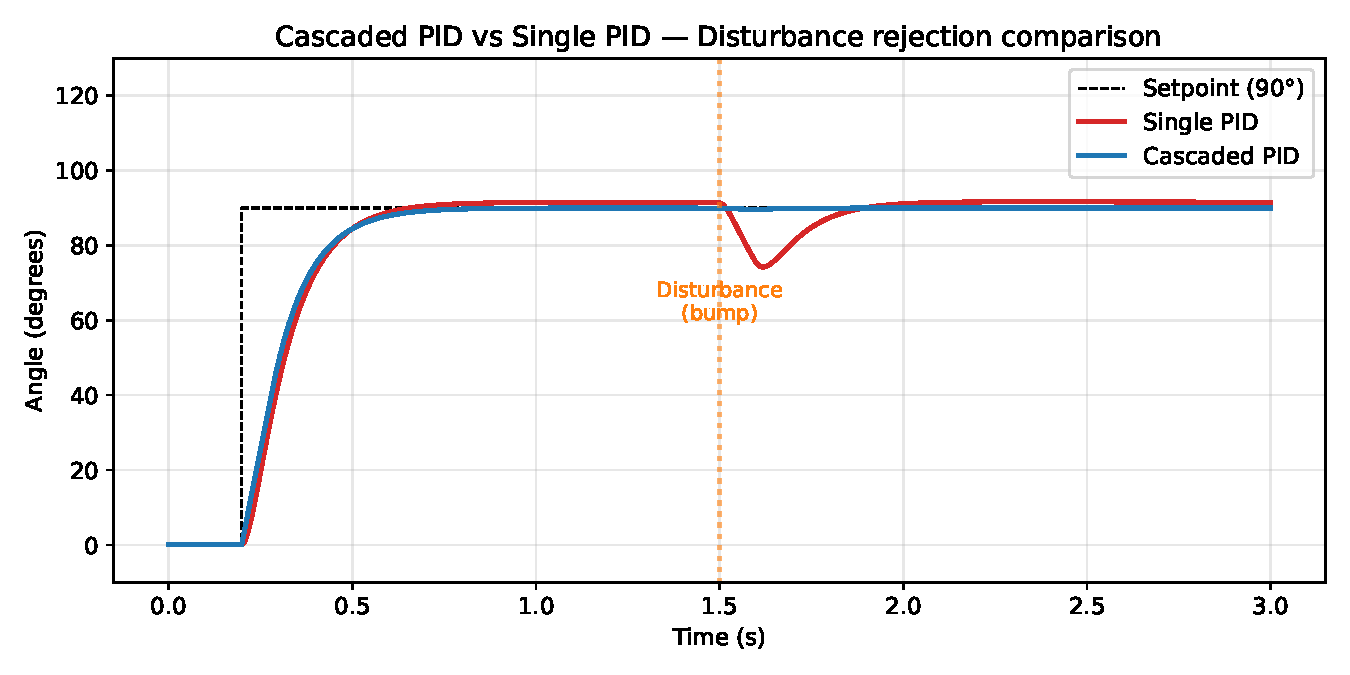
\includegraphics[width=\textwidth]{cascaded_pid.pdf}
\caption{级联PID（蓝色）与单回路PID（红色）在云台电机上的对比。两者都跟踪90°设定值，但当扰动在 $t=1.5$s 发生时，级联架构恢复得更快，因为内速度环承受了冲击。}
\end{figure}

\subsection{PID 架构：单级、串级与并联串级}

上述案例分析展示了串级 PID 在单轴上相比单回路 PID 的优势。在实际比赛中，机器人通常需要多轴协调控制（例如云台偏航 + 俯仰，底盘 X + Y + 旋转）。本节系统比较三种 PID 架构，并提供相应的代码实现。

\subsubsection{架构一：单级 PID}

最简单的架构：每个轴一个 PID 控制器，从位置误差直接输出电机电压。

\[
u(t) = K_p e(t) + K_i \int_0^t e(\tau)\,d\tau + K_d \frac{de(t)}{dt}, \qquad e(t) = r(t) - y(t)
\]

\textbf{优点：}实现简单，每个轴只需整定一组增益，计算开销最小。

\textbf{局限：}单个控制器需同时处理快速动态（电气/电流）和慢速动态（机械/位置）。这种耦合使得整定困难——为加快跟踪而增大增益往往会引发振荡。抗扰动能力较弱，因为控制器只有在扰动传播到位置输出后才能做出反应。

\subsubsection{架构二：串级（级联）PID}

每个轴两个嵌套回路：外环产生速度（或电流）设定值，输入内环。

\[
\omega_{\text{cmd}} = \text{PID}_{\text{外环}}\bigl(\theta_{\text{ref}} - \theta\bigr), \qquad
u = \text{PID}_{\text{内环}}\bigl(\omega_{\text{cmd}} - \omega\bigr)
\]

\textbf{优点：}每个回路只处理一层动态，使整定变得简单（先内环，后外环）。内环在扰动传递到外环之前便将其抑制，抗扰动性能显著提升。此外，外环输出有界的速度指令，天然起到限幅保护作用，避免突然的大力矩。

\textbf{设计准则：}内环带宽应为外环的 5--10 倍。从外环的视角看，内环应表现为一个简单的一阶系统（即整定良好、响应快、无超调）。整定时由内而外：先在外环断开的条件下稳定并优化内环，再闭合外环。

\subsubsection{架构三：并联串级 PID（多轴协同）}

在多轴系统（如偏航 + 俯仰的云台）中，每个轴各运行一个串级 PID 控制器，各轴\textit{并行}运行。各轴共享传感器数据，并可选择性地加入轴间耦合补偿。

\textbf{耦合问题的重要性：}在云台上，俯仰运动会改变重心位置，对偏航轴产生力矩扰动。若不加以补偿，偏航控制器会将其视为未知扰动，反应迟缓。通过加入耦合前馈项，偏航控制器可预判俯仰运动并主动补偿：

\[
u_{\text{偏航}} = \text{串级PID}_{\text{偏航}}(\cdot) + k_{\text{耦合}} \cdot \dot{\theta}_{\text{俯仰}}
\]

\begin{verbatim}
    // 含轴间耦合补偿的并联串级 PID
    struct GimbalController {
        CascadedPID yaw;
        CascadedPID pitch;
        float cross_yaw_from_pitch = 0.0f;  // 耦合增益

        struct Output { float yaw_voltage; float pitch_voltage; };

        Output update(float yaw_ref, float yaw_pos, float yaw_vel,
                      float pitch_ref, float pitch_pos, float pitch_vel,
                      float yaw_vel_ff = 0, float pitch_vel_ff = 0) {
            // 耦合补偿：俯仰角速度对偏航的扰动
            float cross_comp = cross_yaw_from_pitch * pitch_vel;

            float u_pitch = pitch.update(pitch_ref, pitch_pos,
                                         pitch_vel, pitch_vel_ff);
            float u_yaw   = yaw.update(yaw_ref, yaw_pos,
                                       yaw_vel, yaw_vel_ff)
                          + cross_comp;
            return {u_yaw, u_pitch};
        }

        void reset() { yaw.reset(); pitch.reset(); }
    };
\end{verbatim}

\subsubsection{架构对比总结}

\begin{center}
\begin{tabular}{lccc}
\toprule
 & \textbf{单级 PID} & \textbf{串级 PID} & \textbf{并联串级} \\
\midrule
每轴回路数 & 1 & 2 & 2 \\
整定难度 & 中等 & 低（分层整定） & 低（分层整定） \\
抗扰动能力 & 慢 & 快 & 快 \\
轴间耦合处理 & 无 & 无 & 可补偿 \\
代码复杂度 & 最低 & 适中 & 适中 \\
典型应用 & 简单执行器 & 单轴云台 & 多轴云台 \\
\bottomrule
\end{tabular}
\end{center}

\begin{figure}[H]
\centering
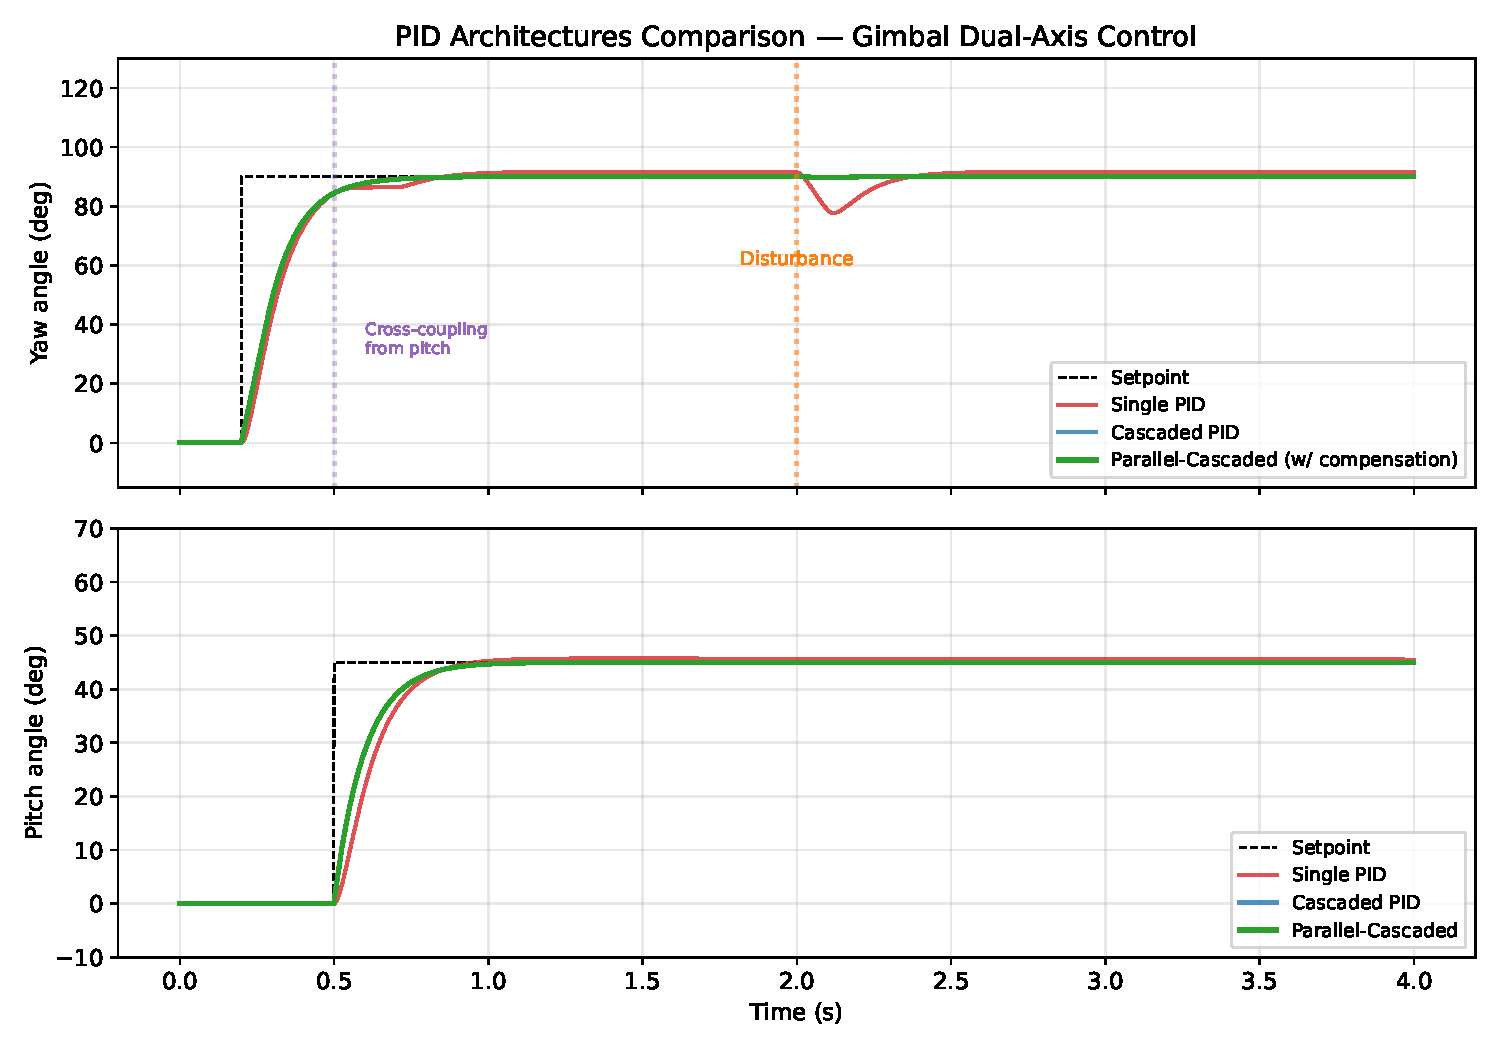
\includegraphics[width=\textwidth]{pid_architectures.pdf}
\caption{双轴云台上的 PID 架构对比。上图：偏航轴，在 $t=2$s 处受到外部扰动，在 $t=0.5$s 处受到来自俯仰运动的耦合扰动。下图：俯仰轴。含耦合补偿的并联串级架构（绿色）在扰动和耦合同时存在时提供了最平稳的偏航响应。}
\end{figure}

\textbf{实践建议：}对于任何具有多个受控轴的系统，建议采用并联串级架构。额外的代码复杂度极小（仅需一个结构体封装两个 \texttt{CascadedPID} 对象），而分层整定和耦合补偿带来的性能提升却十分显著。

\begin{mdframed}[linewidth=1pt, innertopmargin=10pt, innerbottommargin=10pt]
\textbf{实践案例：两轮自平衡车（并联 PID）}

\vspace{0.3em}
两轮自平衡机器人（如 Segway）是经典的\textit{并联}多环控制问题。至少需要同时控制三个目标：平衡（倾斜角）、速度和偏航（转向）。每个目标各有一个控制器，它们的输出在电机层面\textit{相加}。

\begin{itemize}[nosep]
    \item \textbf{平衡环（快）：}对 IMU 测量的倾斜角 $\phi$ 进行 PD 控制。这是最关键的环——必须以 $\geq 500$\,Hz 运行，毫秒级响应。输出是施加给两个轮子的同向力矩。
    \item \textbf{速度环（中）：}对轮速（编码器）进行 PI 控制。参考值来自用户操纵杆。输出叠加到平衡力矩上。该环防止机器人在保持平衡的同时漂移。
    \item \textbf{偏航环（慢）：}对偏航角速度（陀螺仪）进行 P 控制。输出是\textit{差动}力矩——左轮正、右轮负（或反之）——用于转向。
\end{itemize}

\textbf{电机指令融合：}
\[
u_{\text{left}}  = \underbrace{\tau_{\text{balance}}}_{\text{PD on } \phi} + \underbrace{\tau_{\text{velocity}}}_{\text{PI on } v} + \underbrace{\tau_{\text{yaw}}}_{\text{P on } \dot{\psi}}
\]
\[
u_{\text{right}} = \tau_{\text{balance}} + \tau_{\text{velocity}} - \tau_{\text{yaw}}
\]

$\tau_{\text{yaw}}$ 的符号翻转实现了差速转向。每个环独立整定：先调平衡（机器人得先站住才能动），再调速度，最后调偏航。
\end{mdframed}

\subsubsection{并联 PID 的输出冲突问题}

当多个 PID 控制器并联运行、输出相加到同一个执行器时，它们可能\textit{互相打架}。这是并联架构的根本风险。

\textbf{平衡车中的冲突。}考虑平衡环命令``向前倾以保持直立''，而速度环同时命令``向后倾以减速''。两者在各自的视角下都是正确的，但叠加后的输出相互抵消，给电机留下一个微弱、混乱的指令。最坏情况下，两个环互相振荡：速度环制造了一个倾斜扰动，平衡环纠正它，进而改变了速度，又触发速度环——形成环间极限环振荡。

\textbf{原因分析：}在串级架构中，外环\textit{只和}内环对话，内环\textit{只和}执行器对话。层级结构从设计上就避免了冲突。而并联架构中，所有环都直接和执行器对话，因此它们的控制目标必须\textit{天然兼容}。当目标不兼容时，叠加输出就会变得混乱。

\textbf{缓解策略：}
\begin{enumerate}[nosep]
    \item \textbf{带宽分离。}确保每个环工作在不同的频率带：最快的环（平衡）在高频主导，最慢的环（偏航）只在低频起作用。冲突指令在时间尺度上分离，因此不会干扰。
    \item \textbf{优先级限幅。}对较慢环的输出进行限幅，使其不能压过较快的安全关键环。例如，限制 $|\tau_{\text{velocity}}|$ 使其不超过 $|\tau_{\text{balance}}|$ 的某个比例。
    \item \textbf{输出额度分配。}为每个环预留固定的执行器输出范围：例如 60\% 给平衡，30\% 给速度，10\% 给偏航。这保证了任何一个环都不会``饿死''另一个环。
    \item \textbf{转化为串级。}如果冲突持续存在，重构控制器，使速度环输出\textit{倾斜角给定值}给平衡环，而不是直接输出与之竞争的力矩。这从设计上消除了冲突——代价是增加了环间耦合。
\end{enumerate}

\textbf{经验法则：}当被控变量在\textit{物理上正交}时（例如平衡车上的平衡 vs.\ 偏航——一个是矢状面，另一个是侧向），并联 PID 效果良好。当两个环试图控制共享同一执行器自由度的变量时（例如平衡和速度都需要矢状面力矩），并联 PID 就会力不从心。

\subsubsection{思考题：串级 PID 的内环 $K_p$ 等价于外环 $K_d$ 吗？}

考虑一个位置--速度串级系统。外环输出的速度给定值正比于位置误差：$v_{\text{ref}} = K_p^{\text{outer}} (r - y)$。内环跟踪该速度。再看单级位置 PID：微分项产生 $K_d \cdot \dot{e} \approx -K_d \cdot \dot{y}$，这是一个正比于速度的反馈。

\textbf{它们等价吗？}\textit{几乎等价，但不完全。}在稳态线性分析中，外环 $K_p$ 通过理想内环速度回路产生的效果类似于位置误差上的 $K_d$。具体来说，如果内环增益为 1 且无动态延迟（即瞬时速度跟踪），则：
\[
u = K_p^{\text{inner}} \bigl(K_p^{\text{outer}}(r-y) - \dot{y}\bigr)
\]
展开后包含类似 $K_p \cdot e + K_d \cdot (-\dot{y})$ 的项，其中 $K_d \approx K_p^{\text{inner}}$。

\textbf{但串级在实践中更优，因为：}
\begin{enumerate}[nosep]
    \item 内环有自己的\textit{积分项}，可以消除速度层面的扰动（摩擦、负载变化），而无需依赖外环。
    \item 内环对外环指令进行\textit{带宽限制}，防止外环要求物理上不可能的加速度。裸露的 $K_d$ 没有这种保护——它放大高频噪声，可能导致执行器饱和。
    \item 内环使用的是\textit{测量}的速度信号，而非数值微分。微分放大噪声；直接测量不会。
\end{enumerate}

\textbf{结论：}微分项和内环比例增益在概念上是相关的——两者都注入了与速度相关的阻尼。但串级架构提供的噪声抑制、速度层面的扰动抑制以及隐式速率限制，是裸露的 $K_d$ 项无法匹敌的。

\newpage

%=============================================================================
\section{离散化与实现}
%=============================================================================

纸上（或 MATLAB 里）的连续时间控制器已经设计好了。接下来要把它塞进 STM32 的 1 kHz 定时器中断里跑起来。如果你把连续域设计的 $K_p = 100$ 的 PID 直接塞进 1 ms 定时器，会发生什么？答案取决于你怎么离散化——选错了方法，稳定的控制器可能变成不稳定的。

\subsection{从连续到离散}

连续时间传递函数 $C(s)$ 得先转成离散时间的 $C(z)$，才能写进代码。方法有好几种，各有各的取舍。

\subsubsection{零阶保持（Zero-Order Hold，ZOH）}

零阶保持（ZOH）假设输入在两次采样之间保持不变——DAC（数模转换器，Digital-to-Analog Converter，把单片机里的数字量转换成电压的芯片）就是这么工作的。物理上最精确的离散化方法。

\textbf{核心思想：}在采样时刻之间，控制信号保持不变。我们精确计算连续系统在这种分段常数输入下的响应。

对于一阶系统 $G(s) = \frac{a}{s + a}$，采样周期为 $T_s$：
\begin{equation}
G(z) = \frac{1 - e^{-aT_s}}{z - e^{-aT_s}}
\end{equation}

推导思路：ZOH 离散化公式为 $G(z) = (1-z^{-1})\mathcal{Z}\{G(s)/s\}$。对于 $G(s) = a/(s+a)$，连续阶跃响应为 $y(t) = 1 - e^{-at}$；采样得 $y[n] = 1 - e^{-anT_s}$；取 Z 变换再乘以 $(1-z^{-1})$ 即得结果。

\textbf{适用场景：}当你希望离散系统在采样时刻与连续系统完全吻合时。MATLAB 的 \texttt{c2d(sys, Ts, 'zoh')} 使用的就是这种方法。

\textbf{缺点：}对高阶系统，转换公式可能相当复杂，通常借助软件工具完成，不适合手算。

\subsubsection{双线性变换（Tustin Transform，也称 Bilinear Transform）}

我们能不能找到一种更聪明的映射，让连续系统的频率特性尽量保留下来？答案是用梯形积分近似——这就是双线性变换的由来。

双线性变换（Tustin 变换）将 $s$ 替换为：
\begin{equation}
s \leftarrow \frac{2}{T_s} \cdot \frac{z - 1}{z + 1}
\end{equation}

纯粹的代数代换：把连续传递函数里的 $s$ 全换成上面的表达式，化简就完了。

\textbf{示例：}一阶低通滤波器 $H(s) = \frac{\omega_c}{s + \omega_c}$ 变换后为：
\begin{equation}
H(z) = \frac{\omega_c T_s (z + 1)}{(2 + \omega_c T_s) z + (\omega_c T_s - 2)}
\end{equation}

\textbf{双线性变换流行的原因：}
\begin{itemize}
    \item 对低阶系统可以手算，计算简单。
    \item 保持稳定性：稳定的连续系统映射到稳定的离散系统。
    \item 低频段的频域匹配效果好。
\end{itemize}

\textbf{注意事项：}在高频处（接近奈奎斯特频率），双线性变换会引入\textbf{频率翘曲（frequency warping）}——离散滤波器的截止频率相对于连续设计发生偏移。使用\textbf{预翘曲（pre-warping）}来修正这一问题：
\begin{equation}
\omega_{\text{pre-warped}} = \frac{2}{T_s} \tan\left(\frac{\omega_c T_s}{2}\right)
\end{equation}

双线性变换将整个连续频率轴 $\omega \in [0, \infty)$ 压缩到有限弧段 $\omega_d \in [0, \pi/T_s)$ 上，高频被严重压缩。映射关系为 $\omega = \frac{2}{T_s}\tan\frac{\omega_d T_s}{2}$。预翘曲就是反过来：给双线性变换喂一个"拉伸"后的频率，使目标频率 $\omega_c$ 在压缩后精确落到正确位置。

在连续设计中用 $\omega_{\text{pre-warped}}$ 替换 $\omega_c$，再应用双线性变换。

\subsubsection{极零点匹配法（Matched Pole-Zero Method）}

该方法使用 $z = e^{sT_s}$ 将连续系统的极点和零点映射到 $z$ 域。它能较好地保留时域响应特性。

\textbf{适用场景：}当匹配瞬态响应比匹配频率响应更重要时。在实践中不如 ZOH 或双线性变换常用。

\textbf{小结：}对于大多数竞赛应用，\textbf{双线性变换是首选方法}。简单、稳定、精度足够。需要精确的采样时刻匹配时用 ZOH。如果你使用 MATLAB，直接用 \texttt{c2d()} 让它处理数学细节即可。

\begin{figure}[H]
\centering
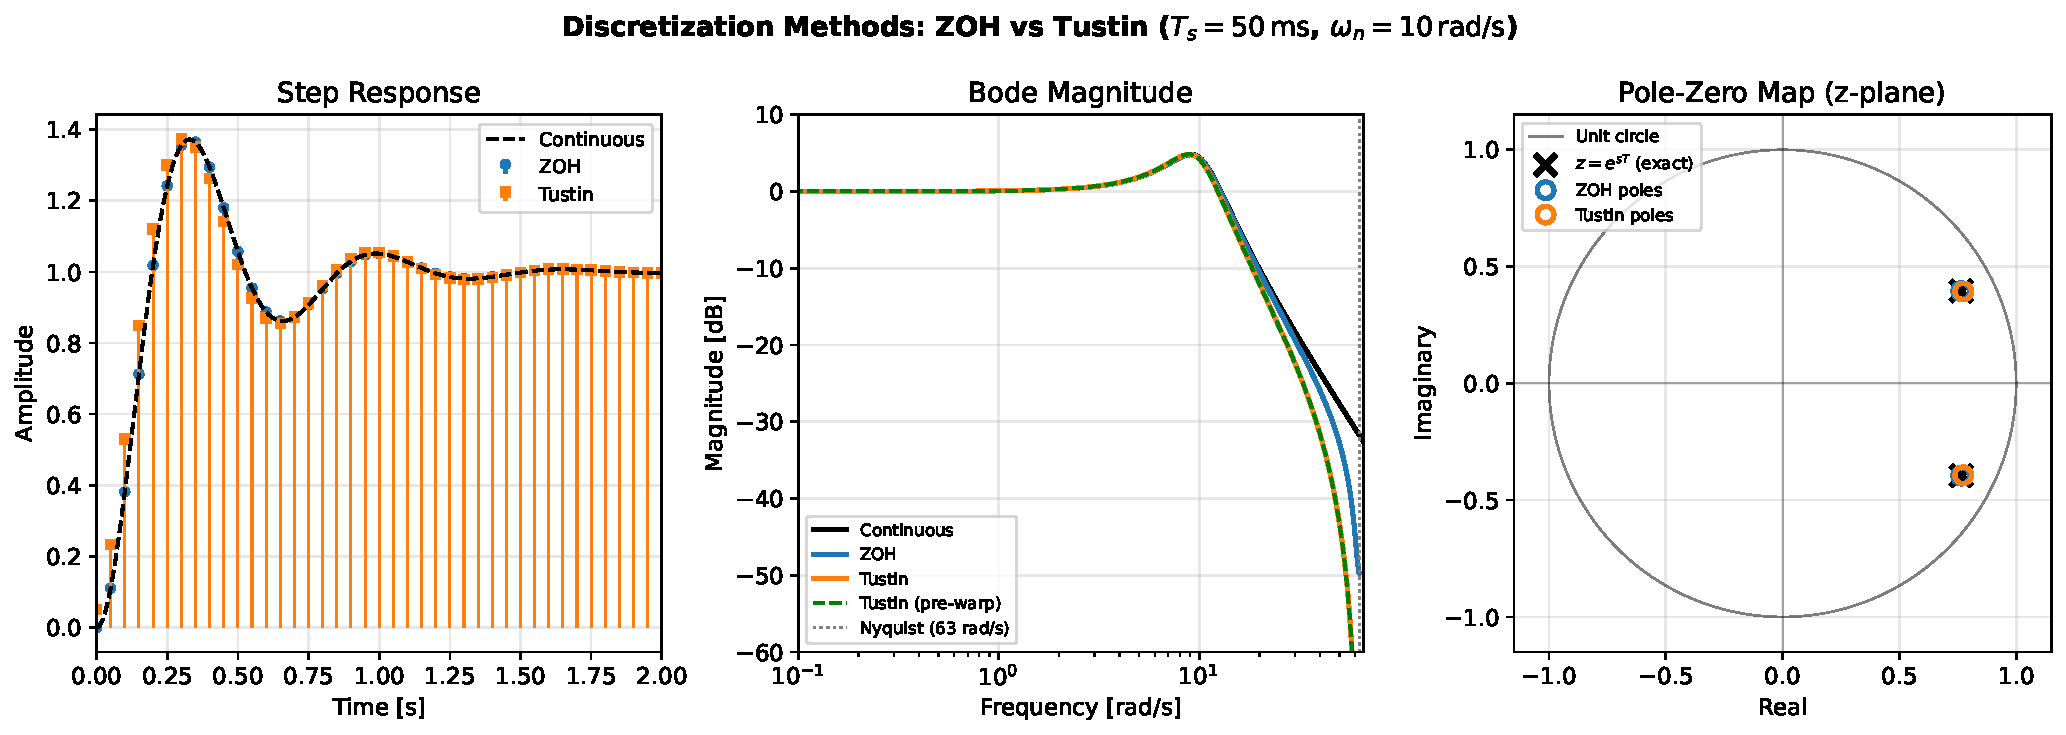
\includegraphics[width=\textwidth]{discretization_comparison.pdf}
\caption{ZOH 与双线性变换对欠阻尼二阶系统的离散化对比（$\omega_n = 10$~rad/s，$\zeta = 0.3$，$T_s = 50$~ms）。左图：阶跃响应——ZOH 在采样时刻与连续系统完全吻合。中图：Bode 幅频图——双线性变换在奈奎斯特频率附近出现频率翘曲；预翘曲（绿色）修正了这一问题。右图：极零点图，展示了各方法如何将连续极点映射到 $z$ 平面。}
\end{figure}

\subsection{数字滤波器结构：FIR 与 IIR}

学会了如何将连续时间设计转换为离散时间传递函数之后，自然而然的下一个问题是：得到的数字滤波器在代码中到底长什么样？有两种基本结构：\textbf{FIR} 和 \textbf{IIR}。理解二者的区别，对于在单片机上选择正确的实现方式至关重要。

\subsubsection{FIR（有限冲激响应，Finite Impulse Response）}

FIR 滤波器的输出仅由当前和过去的输入采样的加权和决定——没有反馈：

\begin{equation}
y[n] = \sum_{k=0}^{M} b_k \, x[n-k]
\end{equation}

$z$ 域表示：
\begin{equation}
H(z) = \sum_{k=0}^{M} b_k \, z^{-k}
\end{equation}

FIR 滤波器\textbf{只有零点}（除了 $z = 0$ 处的平凡极点外没有极点），这带来两个重要性质：
\begin{itemize}
    \item \textbf{永远稳定}——没有反馈就不存在失控振荡的风险。
    \item \textbf{可以实现线性相位}——只要系数对称（$b_k = b_{M-k}$），每个频率分量的延迟相同，信号波形被完美保持。
\end{itemize}

代价是\textbf{滤波器阶数}：要实现陡峭的截止，可能需要 $M = 50$--$200$ 个抽头（tap），这意味着要存储那么多过去的采样值，每个输出采样要做那么多次乘法。

\textbf{常用 FIR 设计方法：}
\begin{itemize}
    \item \textbf{窗函数法（Window Method）}——截断理想冲激响应，乘以窗函数（汉明窗 Hamming、布莱克曼窗 Blackman、凯泽窗 Kaiser）以减少频谱泄漏（由于冲激响应被突然截断，能量从一个频率格"洒"到相邻频率格的现象）。
    \item \textbf{频率采样法（Frequency Sampling）}——在 DFT 采样点上指定期望的幅度响应，再做逆变换。
    \item \textbf{Parks--McClellan（Remez）算法}——一种最优算法，最小化最大逼近误差（等纹波设计）。
\end{itemize}

\subsubsection{IIR（无限冲激响应，Infinite Impulse Response）}

IIR 滤波器\textit{同时}使用过去的输入和过去的输出——存在反馈通路：

\begin{equation}
y[n] = \sum_{k=0}^{M} b_k \, x[n-k] \;-\; \sum_{k=1}^{N} a_k \, y[n-k]
\end{equation}

$z$ 域表示：
\begin{equation}
H(z) = \frac{\displaystyle\sum_{k=0}^{M} b_k \, z^{-k}}
            {1 + \displaystyle\sum_{k=1}^{N} a_k \, z^{-k}}
     = \frac{B(z)}{A(z)}
\end{equation}

IIR 滤波器\textbf{既有极点又有零点}。极点使得用很低的阶数就能实现很尖锐的频率选择性（一个 4 阶 IIR 可以超过一个 50 阶 FIR），但也带来风险：
\begin{itemize}
    \item \textbf{可能不稳定}——如果任何极点位于单位圆外（$|z| > 1$），输出将无界增长。
    \item \textbf{非线性相位}——不同频率的延迟不同，信号波形会失真。
    \item \textbf{系数敏感}——在定点单片机上，系数的舍入可能将极点推出单位圆，导致不稳定。
\end{itemize}

\textbf{经典 IIR 设计}从模拟原型出发，使用我们刚讲过的方法（双线性变换、ZOH 等）映射到离散时间：
\begin{itemize}
    \item \textbf{巴特沃斯（Butterworth）}——通带最大平坦，单调滚降。"香草味"选项；听起来平淡无奇，但 80\% 的情况下它就是正确的默认选择。
    \item \textbf{切比雪夫 I 型（Chebyshev Type~I）}——通带等纹波，阻带单调。同阶数下比巴特沃斯过渡更陡，代价是通带有纹波。
    \item \textbf{切比雪夫 II 型（Chebyshev Type~II）}——通带单调，阻带等纹波。不太常见，但在通带平坦度更重要时很有用。
    \item \textbf{椭圆滤波器（Elliptic / Cauer）}——通带和阻带\textit{都是}等纹波。在给定阶数下过渡带最窄，但到处都有纹波。
\end{itemize}

注意：上一小节介绍的双线性变换和冲激不变法（在离散时刻对模拟滤波器的冲激响应进行采样，保留了时域波形但在高频处可能出现混叠），正是将这些模拟原型转换为离散 IIR 滤波器的工具。

\subsubsection{FIR vs.\ IIR：正面对比}

\begin{center}
\begin{tabular}{lll}
\toprule
\textbf{特性} & \textbf{FIR} & \textbf{IIR} \\
\midrule
稳定性 & 永远稳定 & 需验证（极点在单位圆内） \\
相位 & 可实现线性相位 & 非线性相位 \\
实现陡峭截止的阶数 & 高（50--200+） & 低（典型 4--10） \\
每个采样的计算量 & $M+1$ 次乘法 & $M+N+1$ 次，但 $M,N$ 很小 \\
延迟 & 较高（滤波器更长） & 较低 \\
能否从模拟原型设计 & 否 & 能（巴特沃斯、切比雪夫、椭圆） \\
系数量化敏感度 & 低 & 高 \\
\bottomrule
\end{tabular}
\end{center}

\subsubsection{实用选择指南与 Biquad 实现}

\begin{itemize}
    \item 需要\textbf{线性相位}（音频、对称脉冲整形、通信）？用 \textbf{FIR}。
    \item 需要\textbf{陡峭截止且计算量小}（实时控制回路、资源受限的 MCU）？用 \textbf{IIR}。
    \item 需要\textbf{保证稳定}且不想仔细分析？用 \textbf{FIR}。
    \item 对于高阶 IIR 滤波器，\textbf{一定}要用级联二阶段（biquad）实现，以降低系数敏感度：
\end{itemize}
\begin{equation}
H(z) = \prod_{i=1}^{L}
       \frac{b_{0i} + b_{1i}\,z^{-1} + b_{2i}\,z^{-2}}
            {1   + a_{1i}\,z^{-1} + a_{2i}\,z^{-2}}
\end{equation}

每一段是一个"biquad"——一个二阶 IIR 滤波器，实现简单、数值稳定。$L$ 个 biquad 级联得到 $2L$ 阶滤波器，同时将系数量化效应限制在每一段内部。

\textbf{示例：C 语言中的 biquad（转置直接 II 型）}
\begin{verbatim}
    // 一个 biquad 段——两个状态变量，数值稳定
    float biquad(float x, float *state,
                 float b0, float b1, float b2,
                 float a1, float a2) {
        float y = b0*x + state[0];
        state[0] = b1*x - a1*y + state[1];
        state[1] = b2*x - a2*y;
        return y;
    }
\end{verbatim}

\vspace{0.5em}
\begin{mdframed}[linewidth=1pt, innertopmargin=10pt, innerbottommargin=10pt]
\textbf{快速决策流程}

\vspace{0.3em}
\begin{enumerate}[nosep]
    \item 应用对相位敏感吗（例如波形对称性很重要）？$\rightarrow$ \textbf{FIR}，使用对称系数。
    \item 实时计算很紧张吗（MCU 运行快速控制回路）？$\rightarrow$ \textbf{IIR}（巴特沃斯或切比雪夫），用级联 biquad 实现。
    \item 滤波器阶数适中且平台内存充足？$\rightarrow$ 两者皆可；默认选 \textbf{FIR}，更简单更鲁棒。
    \item 需要在给定阶数下实现最陡的过渡带？$\rightarrow$ \textbf{IIR}，使用椭圆原型。
\end{enumerate}

\textbf{机器人领域的经验法则：}嵌入式系统上大多数传感器平滑滤波器都是低阶 IIR（通常只是 1 阶或 2 阶巴特沃斯）。FIR 滤波器在音频处理、通信以及任何线性相位不可妥协的应用中大放异彩。
\end{mdframed}

\subsection{定点与浮点运算}

竞赛中常用的微控制器（STM32F1、STM32F4）通常配有硬件浮点单元（FPU）。如果你的芯片有 FPU，\textbf{就用浮点}。更简单、更不容易出错，对大多数控制循环来说也足够快。

如果你不得不使用没有 FPU 的微控制器，或者需要追求极致速度，就需要用到\textbf{定点运算（fixed-point arithmetic）}。其思路是用缩放整数来表示小数：
\begin{equation}
\text{fixed\_value} = \text{float\_value} \times 2^Q
\end{equation}

其中 $Q$ 是小数位数。例如，在 Q16 格式中，数值 3.14 存储为 $3.14 \times 65536 = 205{,}888$。

\textbf{常见陷阱：}
\begin{itemize}
    \item 溢出：两个 Q16 数相乘会产生 Q32 结果，必须右移回位。
    \item 范围与精度的取舍：小数位越多，精度越高，但表示范围越小。
    \item 积分累积：PID 中的积分项在定点运算中很容易溢出。
\end{itemize}

\textbf{建议：}除非有充分理由，否则使用 32 位浮点。STM32F4 及以上可以在一个时钟周期内完成单精度浮点运算。

\vspace{0.5em}
\begin{mdframed}[linewidth=1pt, innertopmargin=10pt, innerbottommargin=10pt]
\textbf{计算速度为何直接决定控制性能}

\vspace{0.3em}
许多初学者认为，只要算法``正确''，控制就能正常工作。这忽略了一个关键事实：\textit{所有控制算法都必须在采样周期 $T_s$ 内完成执行。}如果计算时间超过 $T_s$，控制器将错过截止时间，下一周期被延迟，等效控制频率降低。最坏情况下，系统可能变得不稳定。

\textbf{具体示例。}假设速度环以 1~kHz 运行（$T_s = 1$~ms），主控为 168~MHz 的 STM32F407。不同算法的计算耗时如下：

\begin{center}
\begin{tabular}{llll}
\toprule
\textbf{算法} & \textbf{复杂度} & \textbf{大致耗时} & \textbf{能否在 1~ms 内完成？} \\
\midrule
PID（3 次乘加） & $O(1)$ & $\sim$1~$\mu$s & 可以（余量 1000 倍） \\
二阶 IIR 滤波器 & $O(1)$ & $\sim$1~$\mu$s & 可以 \\
卡尔曼滤波器（$4 \times 4$） & $O(n^3)$，$n=4$ & $\sim$20~$\mu$s & 可以（余量 50 倍） \\
LQR（增益矩阵乘法，$4 \times 1$） & $O(n \cdot m)$ & $\sim$2~$\mu$s & 可以 \\
MPC（$N=10$，$n=4$，$m=2$） & $O(N \cdot n^3)$ & $\sim$200--500~$\mu$s & 勉强 \\
EKF（含三角函数） & $O(n^3) + \text{trig}$ & $\sim$50--100~$\mu$s & 可以，但需注意 \\
\bottomrule
\end{tabular}
\end{center}

\textbf{计算超时的后果：}
\begin{itemize}[nosep]
    \item \textbf{丢失更新：}执行器保持上一周期的指令多运行一个周期。系统将此视为增加的时间延迟。回忆淋浴水温的案例（第~4.1 节）：延迟越大，相位裕度越小，系统越接近失稳。
    \item \textbf{$dt$ 不一致：}如果超时是间歇性的（有时快，有时慢），等效 $dt$ 会波动。假定 $dt$ 恒定的积分项和微分项将累积误差。这就是\textit{抖动（jitter）}，其危害往往大于恒定延迟，因为它不可预测。
    \item \textbf{级联失效：}在串级架构中，如果内环超时，外环收到的是过期的速度数据。外环的响应品质下降，抗扰动能力——采用串级控制的核心动机——将大打折扣。
\end{itemize}

\textbf{实际诊断方法。}在 ISR（中断服务例程，Interrupt Service Routine——硬件在每个定时器周期自动调用的函数）的开始和结束处翻转一个 GPIO 引脚（通用输入输出引脚，General-Purpose I/O——可以用代码控制高低电平的数字引脚），用示波器观察脉宽。若脉宽接近 $T_s$，说明已处于危险区域。若脉宽曾超过 $T_s$，则存在必须在调参之前解决的截止时间违规。

\textbf{计算过慢时的应对措施：}
\begin{enumerate}[nosep]
    \item \textbf{降低算法复杂度。}在约束不活跃时用 LQR 替代 MPC；在非线性不严重时用互补滤波器替代 EKF。
    \item \textbf{离线预计算。}LQR 增益、三角函数查找表、MPC 增益序列均可在 MATLAB/Python 中计算后存为常量。
    \item \textbf{降低控制频率。}如果系统带宽允许，将频率从 1~kHz 降至 500~Hz 可使计算预算翻倍。需检查系统时间常数是否允许（回顾：$T_s \leq \tau / 10$）。
    \item \textbf{分层分频。}将耗时的外环以较低频率运行（如 MPC 以 100~Hz），同时保持简单的内环（PID 以 1~kHz）。内环在 MPC 更新间隔内维持控制。
\end{enumerate}

\textbf{核心认识：}最好的算法不是最复杂的算法，而是能在 $T_s$ 内可靠完成且满足性能要求的算法。一个精心调好的 PID 以 1~kHz 运行，永远优于一个在 200~Hz 下超时的 MPC。
\end{mdframed}

\subsection{采样率选择}

控制循环应该跑多快？太慢则无法响应快速扰动；太快则浪费 CPU 时间（且微分项会放大量化噪声）。

\textbf{经验法则：}采样率应为闭环系统带宽的 10--30 倍。

\begin{center}
\begin{tabular}{lll}
\toprule
\textbf{应用场景} & \textbf{带宽} & \textbf{采样率} \\
\midrule
底盘速度 & $\sim$5 Hz & 50--200 Hz \\
云台位置 & $\sim$20 Hz & 200--1000 Hz \\
电机电流环 & $\sim$500 Hz & 5--20 kHz \\
\bottomrule
\end{tabular}
\end{center}

\textbf{实际约束：}你的采样率受以下因素限制：
\begin{itemize}
    \item 传感器更新率（采样速度超过编码器/IMU 的更新速率毫无意义）。
    \item 计算时间（所有控制运算必须在一个采样周期内完成）。
    \item 通信延迟（CAN 总线、SPI、I2C 可能成为瓶颈）。
\end{itemize}

\textbf{重点：}级联控制环（位置 $\to$ 速度 $\to$ 电流）里，内环要比外环快 5--10 倍。电流环 10 kHz、速度环 1 kHz、位置环 200 Hz，是一种典型配置。

\subsection{嵌入式系统实现}

\subsubsection{定时器与中断配置}

在大多数微控制器（STM32 等）上，控制循环运行在\textbf{定时器中断}中。定时器以固定周期 $T_s$ 触发，中断服务例程（ISR）执行控制算法。

\textbf{最佳实践：}
\begin{itemize}
    \item 为每个控制环使用专用硬件定时器。
    \item 通过预分频器和自动重装寄存器设置所需的定时器周期 $T_s$。
    \item ISR \textbf{越短越好}：读传感器、计算输出、设置执行器。不要打印、不要 UART、不要动态内存分配。
    \item ISR 与主循环共享的变量使用 \texttt{volatile} 修饰。
    \item 正确设置中断优先级：电流环 $>$ 速度环 $>$ 位置环。
\end{itemize}

\textbf{示例（STM32 HAL）：}
\begin{verbatim}
void HAL_TIM_PeriodElapsedCallback(TIM_HandleTypeDef *htim) {
    if (htim->Instance == TIM6) {  // 1 kHz control loop
        float measurement = read_encoder();
        float error = setpoint - measurement;
        float output = pid_compute(&pid, error);
        set_motor_pwm(output);
    }
}
\end{verbatim}

\subsubsection{计算延迟与抖动}

\textbf{延迟（Latency）}是从读取传感器到施加输出之间的时间。越小越好。超过 $T_s / 2$ 时，性能会显著下降。

\textbf{抖动（Jitter）}是延迟在每个周期间的变化量。如果你的控制循环通常耗时 10 $\mu$s，但偶尔因被其他中断抢占而耗时 500 $\mu$s，行为就会不一致。抖动往往比固定延迟危害更大。

\textbf{如何减小抖动：}
\begin{itemize}
    \item 给控制定时器分配最高中断优先级。
    \item 避免长时间全局关闭中断。
    \item 在任何 ISR 中不要使用阻塞等待（delay、轮询）。
    \item 对 ISR 执行时间进行剖析（profiling），确保其远小于 $T_s$。
\end{itemize}

\subsubsection{实践中的积分抗饱和}

我们在 PID 章节中讨论过抗饱和（Anti-Windup），但在这里值得特别强调，因为它是真实硬件上 PID ``莫名其妙''异常的头号根源。

\textbf{实践中何时会发生积分饱和？}
\begin{itemize}
    \item 电机电流达到限制（你在命令 20A，但 ESC 上限为 10A）。
    \item PWM 饱和（占空比已到 100\%，无法再增加）。
    \item 机械硬限位（云台碰到限位，轮子被堵转）。
    \item 通信失败（命令发出但未被接收——输出实际上为零）。
\end{itemize}

\textbf{实现检查清单：}
\begin{enumerate}
    \item 将积分项限幅到合理范围。
    \item 将总输出限幅到执行器的实际限制。
    \item 输出饱和时停止积分累积（条件积分）。
    \item 切换控制器或模式时，重置或平滑过渡积分项。
    \item 明确测试积分饱和恢复：命令一个大阶跃，让其饱和，然后反向。
\end{enumerate}

\begin{figure}[H]
\centering
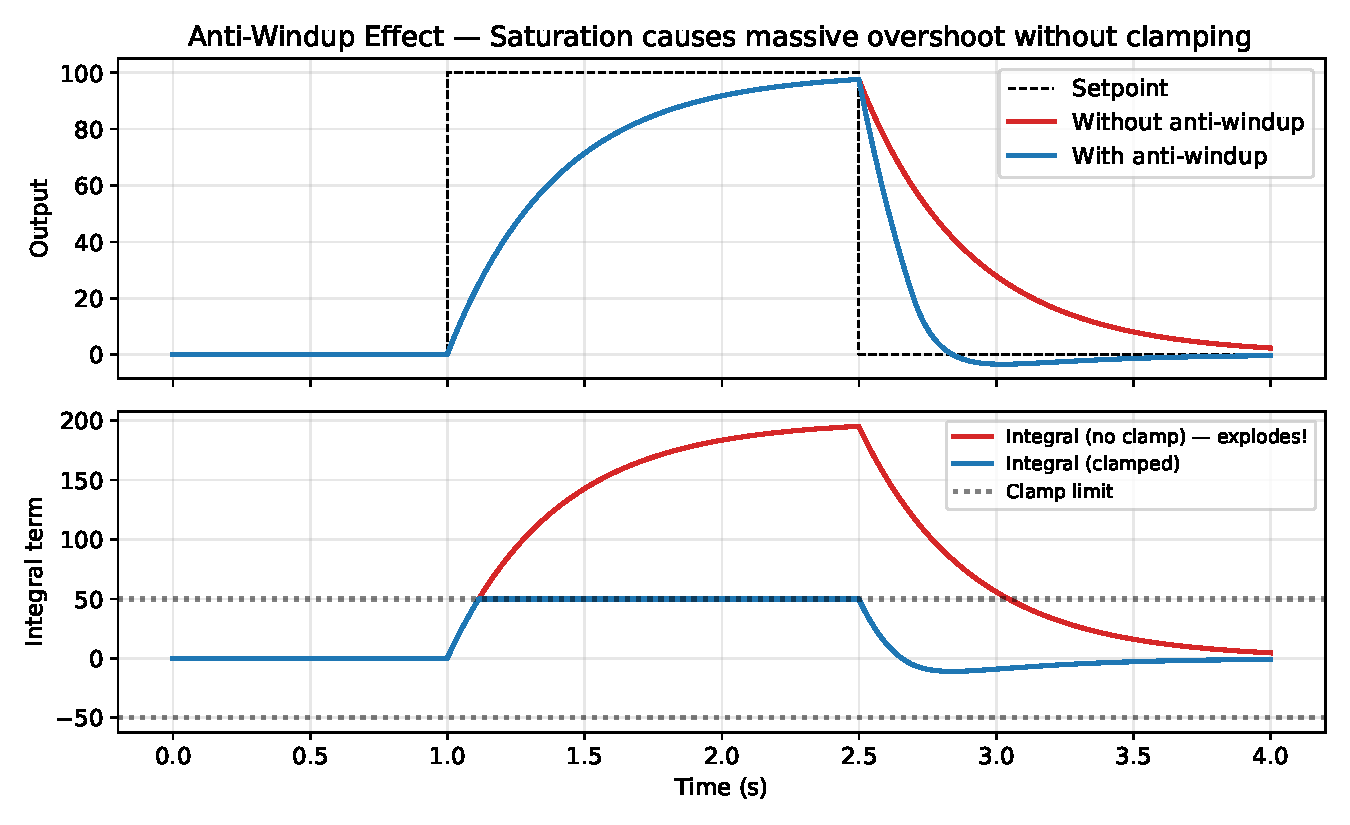
\includegraphics[width=\textwidth]{anti_windup.pdf}
\caption{无抗饱和时（红色），积分项在饱和期间急剧增大，导致设定值切换后出现巨大超调。加入限幅（蓝色）后，积分项保持有界，响应干净利落。}
\end{figure}

\textbf{一个调试故事：}你的机器人轮毂电机在从堵转中恢复后剧烈振荡。你检查了 $K_p$、$K_d$——看起来没问题。你尝试降低增益——有所改善，但系统变得迟钝。真正的原因呢？积分项在堵转期间累积到了一个巨大的值，现在正在朝相反方向猛烈驱动电机。加入积分限幅后立竿见影。这种事情每个人都会遇到，你也会遇到。现在你知道该看哪里了。

\begin{mdframed}[linewidth=1pt, innertopmargin=10pt, innerbottommargin=10pt]
\textbf{从连续 PID 到 STM32 代码：完整流程}

\vspace{0.3em}
本例演示完整流程：从连续时间 PID 出发，离散化，最终在 STM32 定时器中断中实现。

\textbf{第一步：连续 PID。}教科书上的 PID 传递函数：
\[
C(s) = K_p + \frac{K_i}{s} + K_d s
\]
取 $K_p = 6$，$K_i = 0.3$，$K_d = 3$，$T_s = 1\,\text{ms}$（1\,kHz 控制频率）。

\textbf{第二步：Tustin 离散化。}对每一项施加双线性变换 $s \leftarrow \frac{2}{T_s}\frac{z-1}{z+1}$：
\begin{itemize}[nosep]
    \item \textbf{积分项：}$\frac{K_i}{s} \;\to\; \texttt{integral += Ki * Ts * 0.5 * (e + e\_prev)}$（梯形法则）
    \item \textbf{微分项：}$K_d s \;\to\; \texttt{deriv = Kd * (e - e\_prev) / Ts}$（后向差分，更好的做法是作用于测量值）
\end{itemize}

\textbf{第三步：STM32 实现。}
\begin{verbatim}
// In TIM6 interrupt handler, every 1ms:
void TIM6_DAC_IRQHandler(void) {
    HAL_TIM_IRQHandler(&htim6);

    float y = read_encoder();        // measured output
    float r = get_setpoint();        // reference
    float e = r - y;

    // Tustin integral (trapezoidal)
    integral += Ki * Ts * 0.5f * (e + e_prev);
    integral = clamp(integral, -IMAX, IMAX);  // anti-windup

    // Derivative on measurement (avoids derivative kick)
    float dy = (y - y_prev) / Ts;

    // PID output
    float u = Kp * e + integral - Kd * dy;
    u = clamp(u, -UMAX, UMAX);

    set_pwm(u);  // actuator output

    e_prev = e;
    y_prev = y;
}
\end{verbatim}

\textbf{关键实现细节：}
\begin{enumerate}[nosep]
    \item \textbf{微分作用于测量值}（$-K_d \dot{y}$），而非误差（$K_d \dot{e}$）。设定值 $r$ 的阶跃变化会使 $\dot{e}$ 产生无穷大尖峰，猛击执行器。使用 $\dot{y}$ 可避免``微分冲击''。
    \item \textbf{积分限幅}防止执行器饱和时的积分饱和。
    \item \textbf{输出限幅}确保 PWM 在硬件极限范围内。
    \item 在\textbf{无 FPU 的 MCU} 上避免浮点运算——改用定点 Q16 或 Q24 算术。
    \item \textbf{所有状态变量}（\texttt{integral}、\texttt{e\_prev}、\texttt{y\_prev}）为 \texttt{static} 或文件作用域全局变量，在 ISR 调用间持久保存。
\end{enumerate}
\end{mdframed}

\newpage

%=============================================================================
\section{现代控制理论}
%=============================================================================

经典控制（PID、频率响应、根轨迹）已经能走很远了，大多数 SISO 系统它都能漂亮地搞定。但有些问题它够不着：

想象一下：你的平衡车 PID 调好了俯仰角，但每次底盘加速，倾角和速度互相干扰——怎么同时控制两个耦合的量？你的云台跟踪目标很平稳，但编码器坏了一个——怎么从剩余传感器估计出缺失的状态？你的电机要跑得快、又不能超过电流限制——怎么在约束下找到最优解？这些问题都超出了 PID 的能力范围，现代控制理论就是为它们而生的。

它直接在状态空间上干活，线性代数是它的主要武器。

\subsection{状态空间与传递函数的关系}

你在频域里用 Bode 图整形了一个控制器，同事在状态空间里推出了 LQR——你们描述的是同一台机器吗？如何在两种语言之间切换？答案是：可以互相转换。

\textbf{状态空间转传递函数：}
\begin{equation}
G(s) = C(sI - A)^{-1}B + D
\end{equation}

推导：对 $\dot{\mathbf{x}} = A\mathbf{x} + B\mathbf{u}$ 取拉普拉斯变换（零初始条件）得 $s\mathbf{X}(s) = A\mathbf{X}(s) + B\mathbf{U}(s)$，即 $\mathbf{X}(s) = (sI - A)^{-1}B\mathbf{U}(s)$。代入 $\mathbf{Y}(s) = C\mathbf{X}(s) + D\mathbf{U}(s)$ 即得。

\textbf{传递函数转状态空间：}转法不唯一——同一个传递函数可以对应多种状态空间实现。常见的有\textit{可控标准型}（分母系数直接出现在 $A$ 的最后一行，可控性一目了然）和\textit{可观标准型}（分母系数出现在 $A$ 的最后一列，可观性一目了然）。实际工程中，MATLAB 的 \texttt{tf2ss} 可直接给出一种实现；用哪种标准型主要在手算分析时才有区别。

\textbf{关键区别：}传递函数看的是输入-输出行为；状态空间看的是内部动力学。两个系统可以传递函数一模一样，内部结构完全不同——这些额外信息只有状态空间能捕捉到。

\textbf{为什么这很重要：}有些内部模态可能不稳定，但传递函数里看不到（零点把它们抵消了）。状态空间能把这些"隐藏炸弹"揪出来。所以现代控制偏爱状态空间——它看得见全貌。

\subsection{系统性能指标}

\subsubsection{可控性与可观性}

我们来想一个具体的问题：你的双轮平衡车有四个状态（倾角、角速度、位移、速度），但只有一个电机。一个输入能把四个状态都控制好吗？不一定——这取决于系统的\textbf{可控性}。

\textbf{可控性（Controllability）：}「我能否利用现有输入，将每个状态驱动到任意期望值？」

若系统 $(A, B)$ 是可控的，则\textbf{可控性矩阵}（controllability matrix）满秩：
\begin{equation}
\mathcal{C} = \begin{bmatrix} B & AB & A^2B & \cdots & A^{n-1}B \end{bmatrix}, \quad \text{rank}(\mathcal{C}) = n
\end{equation}

\vspace{0.5em}
\begin{mdframed}[linewidth=1pt, innertopmargin=10pt, innerbottommargin=10pt]
\textbf{推导：可控性矩阵为什么长这样}

\vspace{0.3em}
$\mathcal{C} = [B \;\; AB \;\; \cdots \;\; A^{n-1}B]$ 不是凭空变出来的，它从状态递推方程一步步推出来。

\textbf{第一步：逐步展开状态转移。}离散时间系统 $\mathbf{x}[k+1] = A\mathbf{x}[k] + B\mathbf{u}[k]$，从 $\mathbf{x}[0] = \mathbf{0}$ 出发往前推：
\begin{align}
\mathbf{x}[1] &= B\mathbf{u}[0] \\
\mathbf{x}[2] &= A\mathbf{x}[1] + B\mathbf{u}[1] = AB\mathbf{u}[0] + B\mathbf{u}[1] \\
\mathbf{x}[3] &= A^2B\mathbf{u}[0] + AB\mathbf{u}[1] + B\mathbf{u}[2] \\
&\;\vdots \notag \\
\mathbf{x}[n] &= A^{n-1}B\mathbf{u}[0] + A^{n-2}B\mathbf{u}[1] + \cdots + B\mathbf{u}[n-1]
\end{align}

\textbf{第二步：写成矩阵形式。}把输入序列摞成向量：
\begin{equation}
\mathbf{x}[n] = \begin{bmatrix} A^{n-1}B & A^{n-2}B & \cdots & AB & B \end{bmatrix}
\begin{bmatrix} \mathbf{u}[0] \\ \mathbf{u}[1] \\ \vdots \\ \mathbf{u}[n-1] \end{bmatrix}
= \mathcal{C} \cdot \mathbf{u}_{\text{seq}}
\end{equation}

（$\mathcal{C}$ 的列只是换了个顺序，秩不变。）

\textbf{第三步：秩条件。}我们想从零出发到达\textit{任意}目标 $\mathbf{x}[n] \in \mathbb{R}^n$。方程 $\mathcal{C} \cdot \mathbf{u}_{\text{seq}} = \mathbf{x}[n]$ 对任意右端都有解，当且仅当 $\text{rank}(\mathcal{C}) = n$。这就是可控性判据。

\textbf{为什么只要 $n$ 列？}Cayley--Hamilton 定理告诉我们，$A^n$ 可以表示为 $I, A, A^2, \ldots, A^{n-1}$ 的线性组合。所以 $A^n B$ 已经落在 $\text{span}\{B, AB, \ldots, A^{n-1}B\}$ 里了，再往后算也不会增加新信息。

\textbf{连续时间版本：}对 $\dot{\mathbf{x}} = A\mathbf{x} + B\mathbf{u}$，从 $\mathbf{x}(0) = \mathbf{0}$ 出发的可达集合为：
\[
\mathbf{x}(t) = \int_0^{t} e^{A(t-\tau)} B \mathbf{u}(\tau) \, d\tau
\]
把矩阵指数 $e^{A(t-\tau)} = \sum_{k=0}^{\infty} \frac{(t-\tau)^k}{k!} A^k$ 展开，再用 Cayley--Hamilton 把 $n$ 阶及以上的项折叠掉，可达集合还是 $\text{span}\{B, AB, \ldots, A^{n-1}B\}$——同一个可控性矩阵。
\end{mdframed}

\vspace{0.5em}
\begin{mdframed}[linewidth=1pt, innertopmargin=10pt, innerbottommargin=10pt]
\textbf{推导：可观性矩阵为什么长这样}

\vspace{0.3em}
可观性矩阵来自对偶的问题：给定输出序列 $\mathbf{y}[0], \mathbf{y}[1], \ldots$，能否反推初始状态 $\mathbf{x}[0]$？

\textbf{第一步：写出输出方程。}令 $\mathbf{u} = \mathbf{0}$（已知的输入贡献可以事先减掉）。自由响应下：
\begin{align}
\mathbf{y}[0] &= C\mathbf{x}[0] \\
\mathbf{y}[1] &= C\mathbf{x}[1] = CA\mathbf{x}[0] \\
\mathbf{y}[2] &= CA^2\mathbf{x}[0] \\
&\;\vdots \notag \\
\mathbf{y}[n-1] &= CA^{n-1}\mathbf{x}[0]
\end{align}

\textbf{第二步：堆成矩阵方程。}
\begin{equation}
\begin{bmatrix} \mathbf{y}[0] \\ \mathbf{y}[1] \\ \vdots \\ \mathbf{y}[n-1] \end{bmatrix}
= \underbrace{\begin{bmatrix} C \\ CA \\ CA^2 \\ \vdots \\ CA^{n-1} \end{bmatrix}}_{\mathcal{O}} \mathbf{x}[0]
\end{equation}

\textbf{第三步：秩条件。}要从输出序列\textit{唯一}地恢复 $\mathbf{x}[0]$，方程 $\mathcal{O} \cdot \mathbf{x}[0] = \mathbf{y}_{\text{seq}}$ 必须有唯一解。这要求 $\text{rank}(\mathcal{O}) = n$（列满秩）。

\textbf{为什么只要 $n$ 行？}跟可控性同理——Cayley--Hamilton 使得 $CA^n$ 是 $C, CA, \ldots, CA^{n-1}$ 的线性组合，多测几步也不会提供新信息。

\textbf{对偶性一目了然：}可控性问的是"$\mathcal{C}$ 能否把输入空间\textit{映满}状态空间"；可观性问的是"$\mathcal{O}$ 能否把状态空间\textit{区分}成不同的输出"。把一个转置，就得到另一个——这正是对偶性的数学含义：$(A, B)$ 可控 $\Leftrightarrow$ $(A^T, B^T)$ 可观（其中 $B^T$ 扮演 $C$ 的角色）。
\end{mdframed}

\textbf{物理含义：} 若某个状态是不可控的，则任何输入都无法影响它。例如，若你的机器人底盘有一个电机坏了，你就在某些方向上失去了可控性。

\textbf{工作示例：} 考虑一个简化的二维底盘，状态为 $\mathbf{x} = \begin{bmatrix} v_x \\ v_y \end{bmatrix}$（$x$ 和 $y$ 方向的速度），只有一个朝前的电机：
\[
A = \begin{bmatrix} -1 & 0 \\ 0 & -1 \end{bmatrix}, \quad B = \begin{bmatrix} 1 \\ 0 \end{bmatrix}
\]
可控性矩阵：$\mathcal{C} = \begin{bmatrix} B & AB \end{bmatrix} = \begin{bmatrix} 1 & -1 \\ 0 & 0 \end{bmatrix}$。秩为 1，但 $n = 2$。\textbf{不可控！} 该电机只能驱动 $v_x$；没有任何输入能改变 $v_y$。这在物理上很直观：汽车不能横向移动。若添加一个侧向电机（$B = \begin{bmatrix} 1 & 0 \\ 0 & 1 \end{bmatrix}$），可控性便恢复了。

\textbf{可观性（Observability）：}「我能否从现有输出（测量值）中确定每个状态？」

若系统 $(A, C)$ 是可观的，则\textbf{可观性矩阵}（observability matrix）满秩：
\begin{equation}
\mathcal{O} = \begin{bmatrix} C \\ CA \\ CA^2 \\ \vdots \\ CA^{n-1} \end{bmatrix}, \quad \text{rank}(\mathcal{O}) = n
\end{equation}

\textbf{物理含义：} 若某个状态不可观，则无法从测量值中推断出它。例如，若你只测量电机位置而不测量电流，则电流状态可能是不可观的（取决于模型）。

\textbf{可控性-可观性对偶性：} 系统 $(A, B, C)$ 可控，当且仅当对偶系统 $(A^T, C^T, B^T)$ 可观。这一优美的对称性意味着控制器设计技术（极点配置）可以直接移植到观测器设计中。

\textbf{总之：}设计控制器之前查可控性，设计观测器之前查可观性。条件不满足，数学再花哨也白搭——得改硬件（加传感器、修执行器）。

\subsubsection{闭环系统稳定性}

对于具有状态反馈 $\mathbf{u} = -K\mathbf{x}$ 的闭环状态空间系统：
\begin{equation}
\dot{\mathbf{x}} = (A - BK)\mathbf{x}
\end{equation}

当且仅当 $(A - BK)$ 的所有特征值都具有负实部时，系统稳定。增益矩阵 $K$ 正是我们设计用来将这些特征值配置到期望位置的。

\textbf{李雅普诺夫稳定性（Lyapunov stability）：} 一种更通用的稳定性分析工具。若存在一个正定函数 $V(\mathbf{x})$（类似"能量"的函数），且该函数沿轨迹始终递减（$\dot{V} < 0$），则系统稳定。找到这样的 $V$ 就证明了稳定性；找不到并不能证明不稳定（也许只是你没往正确方向找）。

对于线性系统，李雅普诺夫方程为：
\begin{equation}
A^T P + PA = -Q
\end{equation}

推导：选候选 Lyapunov 函数 $V(\mathbf{x}) = \mathbf{x}^T P \mathbf{x}$。沿轨迹 $\dot{\mathbf{x}} = A\mathbf{x}$ 求时间导数：$\dot{V} = \dot{\mathbf{x}}^T P \mathbf{x} + \mathbf{x}^T P \dot{\mathbf{x}} = \mathbf{x}^T(A^T P + PA)\mathbf{x}$。要求 $\dot{V} < 0$（稳定），即需 $A^T P + PA = -Q$（$Q$ 正定）。

若 $Q > 0$ 且解 $P > 0$，则系统稳定。MATLAB 的 \texttt{lyap()} 可直接求解。

\subsection{基于状态空间的控制器设计}

\subsubsection{贝尔曼方程与动态规划：LQR 和 MPC 的核心引擎}

在讲 LQR 和 MPC 之前，得先认识它们背后的数学引擎：\textbf{动态规划（DP）}和\textbf{贝尔曼方程}。如果你打过算法竞赛（USACO、Codeforces、LeetCode），DP 你肯定不陌生——控制理论里的 DP 跟那个是同一个东西，只是换了身衣服。

\textbf{贝尔曼最优性原理（Bellman Principle of Optimality）：}\textit{一个最优策略具有如下性质：无论初始状态和初始决策如何，后续决策对于由第一个决策产生的状态而言，必须构成最优策略。}

说人话：只要你知道从每个中间状态往后的最优策略，就可以枚举所有选项，挑出"这一步的代价 + 之后最优代价"之和最小的那个——最优的第一步就这么定了。

\vspace{0.5em}
\begin{mdframed}[linewidth=1pt, innertopmargin=10pt, innerbottommargin=10pt]
\textbf{热身：网格世界最短路径（你已经熟悉的 DP）}

\vspace{0.3em}
考虑一道经典 DP 问题：你在一个 $n \times n$ 的网格上。从 $(0, 0)$ 出发，目标是到达 $(n{-}1, n{-}1)$。每个格子 $(i, j)$ 有代价 $c(i, j)$。你只能向右或向下移动。求最小代价路径。

\textbf{状态：} 你的位置 $(i, j)$。

\textbf{决策（控制）：} 向右移动或向下移动。

\textbf{代价函数（cost-to-go）：} $V(i, j) = $ 从 $(i, j)$ 到达终点的最小总代价。

\textbf{贝尔曼方程：}
\[
V(i, j) = c(i, j) + \min\{V(i+1, j), \; V(i, j+1)\}
\]

\textbf{边界条件：} $V(n{-}1, n{-}1) = c(n{-}1, n{-}1)$。

\textbf{求解：} 从终点\textit{向后}填表，直到起点。在每个格子处，最优决策是朝代价函数值更小的那个邻居走。总复杂度：$O(n^2)$。

你从第一道 DP 题就一直在这样做了。现在看看换一套词汇会发生什么：

\begin{center}
\begin{tabular}{lll}
\toprule
\textbf{DP（动态规划）} & \textbf{最优控制} & \textbf{含义} \\
\midrule
状态 $(i, j)$ & 状态 $\mathbf{x}_k$ & 当前所在位置 \\
决策（右/下） & 控制输入 $\mathbf{u}_k$ & 下一步做什么 \\
转移 $(i,j) \to (i+1,j)$ & $\mathbf{x}_{k+1} = f(\mathbf{x}_k, \mathbf{u}_k)$ & 物理/动力学规律 \\
步骤代价 $c(i,j)$ & 阶段代价 $\ell(\mathbf{x}_k, \mathbf{u}_k)$ & 该步的惩罚 \\
代价函数 $V(i,j)$ & 值函数 $V_k(\mathbf{x})$ & 最优未来代价 \\
贝尔曼递推 & 贝尔曼方程 & DP 更新规则 \\
向后填表 & 向后 Riccati 递推 & 求解方式 \\
$(i,j)$ 处的最优动作 & 最优策略 $\mathbf{u}_k^* = \pi(\mathbf{x}_k)$ & 每个状态该做什么 \\
\bottomrule
\end{tabular}
\end{center}

\textit{一模一样的算法}。唯一的区别：控制里的「网格」是连续的（状态是实数而不是整数），「决策」是实值的控制输入而不是离散的左/右。

\begin{figure}[H]
\centering
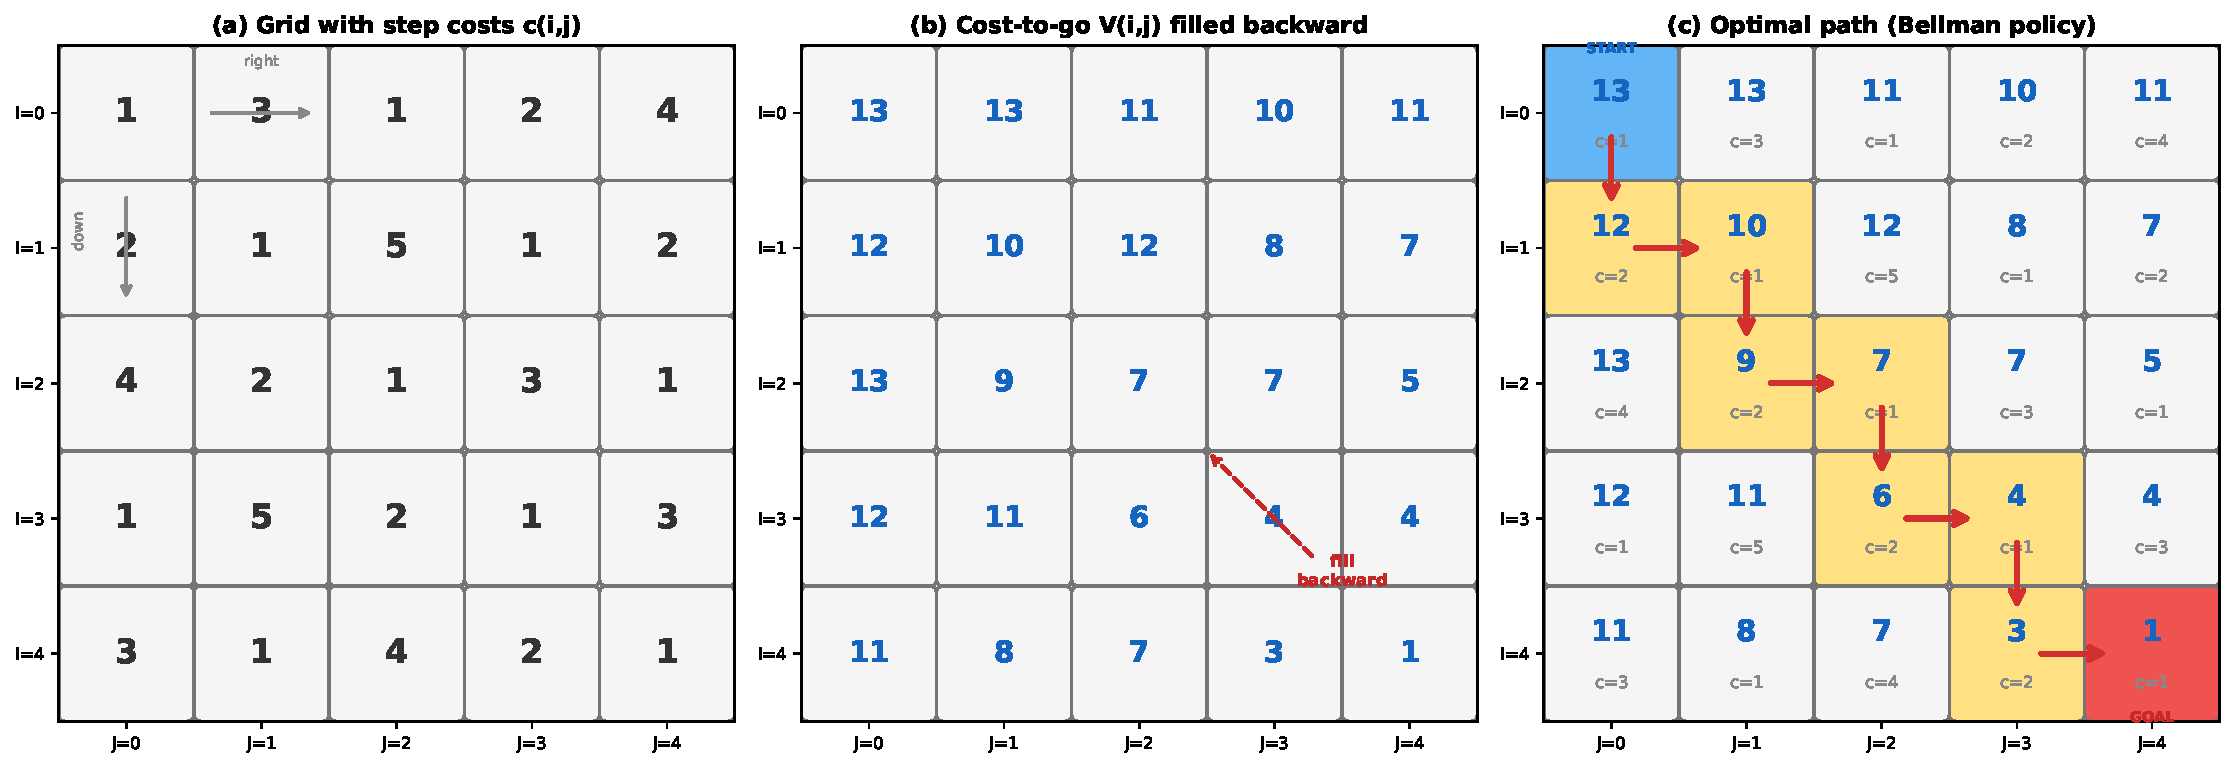
\includegraphics[width=\textwidth]{gridworld_dp.pdf}
\caption{网格世界 DP 示例（$5 \times 5$，移动方式：向右或向下）。(a) 每个格子有步骤代价 $c(i,j)$。(b) 代价函数 $V(i,j)$ 从终点\textit{向后}填充——这就是 DP 表（等价于控制中的 Riccati 递推）。(c) 最优路径（总代价 = 13）遵循贝尔曼策略：在每个格子处，朝 $V$ 值更小的邻居走。将「格子」换成「状态」、「右/下」换成「控制输入」，你就得到了 LQR。}
\end{figure}
\end{mdframed}

\textbf{最优控制的贝尔曼方程（离散时间）：}

给定系统 $\mathbf{x}_{k+1} = f(\mathbf{x}_k, \mathbf{u}_k)$，阶段代价 $\ell(\mathbf{x}_k, \mathbf{u}_k)$ 和终端代价 $\ell_f(\mathbf{x}_N)$，最优代价函数（值函数）满足：

\begin{equation}
V_k(\mathbf{x}) = \min_{\mathbf{u}} \left[ \ell(\mathbf{x}, \mathbf{u}) + V_{k+1}\left(f(\mathbf{x}, \mathbf{u})\right) \right]
\end{equation}

边界条件为 $V_N(\mathbf{x}) = \ell_f(\mathbf{x})$。

第 $k$ 步的最优控制为：
\begin{equation}
\mathbf{u}_k^*(\mathbf{x}) = \arg\min_{\mathbf{u}} \left[ \ell(\mathbf{x}, \mathbf{u}) + V_{k+1}\left(f(\mathbf{x}, \mathbf{u})\right) \right]
\end{equation}

\textbf{这是从时间 $k = N$ 到 $k = 0$ 向后求解的}，就像从终点向起点填 DP 表一样。

\vspace{0.5em}
\begin{mdframed}[linewidth=1pt, innertopmargin=10pt, innerbottommargin=10pt]
\textbf{从网格世界到 LQR：「连续网格」问题}

\vspace{0.3em}
现在想象网格世界变成了连续的。「位置」不再是格子，而是实值状态 $\mathbf{x} \in \mathbb{R}^n$。「移动」不再是右/下，而是实值控制 $\mathbf{u} \in \mathbb{R}^m$。转移是线性的：$\mathbf{x}_{k+1} = A\mathbf{x}_k + B\mathbf{u}_k$。步骤代价是二次的：$\ell(\mathbf{x}, \mathbf{u}) = \mathbf{x}^T Q \mathbf{x} + \mathbf{u}^T R \mathbf{u}$。

代入贝尔曼方程：
\[
V_k(\mathbf{x}) = \min_{\mathbf{u}} \left[ \mathbf{x}^T Q \mathbf{x} + \mathbf{u}^T R \mathbf{u} + V_{k+1}(A\mathbf{x} + B\mathbf{u}) \right]
\]

神奇之处来了：由于动力学是线性的、代价是二次的，值函数\textbf{也是二次的}：$V_k(\mathbf{x}) = \mathbf{x}^T P_k \mathbf{x}$，其中 $P_k$ 是某个矩阵。将此假设代入并对 $\mathbf{u}$ 求导：

\[
\frac{\partial}{\partial \mathbf{u}} \left[ \mathbf{u}^T R \mathbf{u} + (A\mathbf{x} + B\mathbf{u})^T P_{k+1} (A\mathbf{x} + B\mathbf{u}) \right] = 0
\]

求解得：
\begin{align}
\mathbf{u}_k^* &= -\underbrace{(R + B^T P_{k+1} B)^{-1} B^T P_{k+1} A}_{K_k} \, \mathbf{x}_k \\
P_k &= Q + A^T P_{k+1} A - A^T P_{k+1} B (R + B^T P_{k+1} B)^{-1} B^T P_{k+1} A
\end{align}

推导思路：展开 Bellman 方程 $V_k(\mathbf{x}) = \min_{\mathbf{u}}[\mathbf{x}^T Q \mathbf{x} + \mathbf{u}^T R \mathbf{u} + (A\mathbf{x}+B\mathbf{u})^T P_{k+1}(A\mathbf{x}+B\mathbf{u})]$，对 $\mathbf{u}$ 求导令其为零：$2R\mathbf{u} + 2B^T P_{k+1}(A\mathbf{x} + B\mathbf{u}) = 0$，解得 $\mathbf{u}^* = -(R + B^T P_{k+1} B)^{-1} B^T P_{k+1} A \mathbf{x}$。回代即得 $P_k$ 的递推公式。

$P_k$ 的这个向后递推正是\textbf{离散 Riccati 方程}——就是「向后填 DP 表」这一步。当时域 $N \to \infty$ 时，$P_k$ 收敛到常数 $P$，得到稳态的 \textbf{LQR} 增益 $K = (R + B^T P B)^{-1} B^T P A$。

\textbf{对应网格世界的类比：}
\begin{itemize}[nosep]
    \item $P_k$ 是代价矩阵——它告诉你从任意状态出发的「剩余代价」，就像网格中的 $V(i,j)$。
    \item $K_k$ 是第 $k$ 步的最优策略——它告诉你在每个状态该做什么，就像「若 $V(i+1,j) < V(i,j+1)$ 则向右走」。
    \item Riccati 递推就是填 DP 表——同样是 $O(N)$ 的向后遍历。
\end{itemize}
\end{mdframed}

\textbf{与 MPC 的联系：} MPC 使用的是同一套贝尔曼/动态规划框架，只是额外增加了两点：
\begin{enumerate}
    \item 对状态和输入的\textbf{约束}（就像在网格世界中加了墙——某些格子被禁止进入）。
    \item \textbf{滚动时域}：不是从 $k = 0$ 到 $N$ 只求解一次，而是在每个时间步用最新测量值作为新的「起点」重新求解。
\end{enumerate}

约束使贝尔曼方程更难求解（$\min$ 变成了约束优化问题），这就是为什么 MPC 需要二次规划（QP）求解器，或 TinyMPC 的 ADMM 方法。但其底层原理完全相同：向后递推求最优代价函数，向前应用最优策略。

\textbf{与强化学习的联系：} 如果你熟悉强化学习（RL），贝尔曼方程与 RL 中的\textbf{贝尔曼最优性方程}完全一致（$V^*(s) = \max_a [r(s,a) + \gamma V^*(s')]$）。LQR 是线性二次问题的「闭式 RL」。当动力学未知或非线性时，RL 方法（Q-learning、策略梯度）对 LQR 精确计算的解进行近似。

\subsubsection{LQR（线性二次调节器）}

有了贝尔曼/动态规划这套框架，LQR 就水到渠成了——它就是线性二次贝尔曼方程的稳态解。不用手动配极点，只需给一个代价函数，告诉它"性能和控制力度之间怎么平衡"：

为什么选二次型代价？因为它让优化问题有闭式解（Riccati 方程），而且物理上自然——偏差的平方意味着大偏差受到不成比例的惩罚，小偏差几乎不算。

\begin{equation}
J = \int_0^{\infty} \left( \mathbf{x}^T Q \mathbf{x} + \mathbf{u}^T R \mathbf{u} \right) dt
\end{equation}

其中 $Q$ 惩罚状态偏差（$Q$ 大 = 激进跟踪、快速响应），$R$ 惩罚控制代价（$R$ 大 = 温和输入、节省能量）。

最优状态反馈增益为：
\begin{equation}
K = R^{-1} B^T P
\end{equation}

其中 $P$ 是\textbf{连续代数 Riccati 方程（Continuous Algebraic Riccati Equation，CARE）}的解：
\begin{equation}
A^T P + PA - PBR^{-1}B^T P + Q = 0
\end{equation}

不要手动求解这个方程。在 MATLAB 中用 \texttt{lqr(A, B, Q, R)}，在 Python 中用 \texttt{scipy.linalg.solve\_continuous\_are()}。

\textbf{Riccati 方程到底在算什么？}$P$ 是\textbf{最优代价地图}：$P_{ij}$ 编码了状态 $i$ 和 $j$ 交互带来的「未来代价」。哪个状态难搞（拉回零点要花大力气），$P$ 里对应的元素就大。最优增益 $K = R^{-1}B^T P$ 的意思就是：「代价高的状态猛纠，代价低的状态轻拿轻放。」

\textbf{LQR 调参：}关键就在 $Q$ 和 $R$ 怎么选。从 $Q = I$（单位矩阵）和 $R = \rho I$（$\rho$ 为标量）开始。$\rho$ 小意味着激进、快速、消耗大量执行器能量；$\rho$ 大则保守、缓慢、对执行器温和。若要对某些状态施加更大惩罚，增大 $Q$ 对应的对角元素——例如，若你更关心位置而非速度，令 $Q_{11} > Q_{22}$。

\textbf{LQR 在比赛中的优势：}它保证稳定性（如果系统可控），并自带鲁棒性裕度（对 SISO 系统，至少 6 dB 增益裕度和 60\textdegree{} 相位裕度）。它轻松处理 MIMO 系统，且对多轴系统而言，$Q/R$ 调参比 PID 的三个增益更直观。

\textbf{示例：} 平衡两轮机器人。状态为 $\mathbf{x} = [\theta, \dot{\theta}, x, \dot{x}]^T$（倾斜角、倾斜角速度、位置、速度）。PID 方法需要多个嵌套环路；LQR 只需一个 $K$ 矩阵便可搞定。

\textbf{局限性：} LQR 需要完整的状态反馈（$\mathbf{u} = -K\mathbf{x}$），这意味着你需要知道所有状态。如果无法测量所有状态，则需要观测器（见第 6.4 节）。

\subsubsection{优化与凸性简介}

MPC 在每个时间步都要解一道优化题。在深入之前，先建立必要的优化概念。

\textbf{一般优化问题：}
\[
\min_{\mathbf{x}} \; f(\mathbf{x}) \quad \text{subject to} \quad g_i(\mathbf{x}) \leq 0, \;\; h_j(\mathbf{x}) = 0
\]
其中 $f$ 是\textbf{目标函数}（代价），$g_i$ 是\textbf{不等式约束}，$h_j$ 是\textbf{等式约束}。优化器在满足所有约束的前提下，寻找使 $f$ 最小的决策变量 $\mathbf{x}$。

\textbf{什么使问题成为凸问题？}满足以下条件：
\begin{enumerate}[nosep]
    \item 目标函数 $f$ 是\textbf{凸函数}：对任意两点 $\mathbf{a}, \mathbf{b}$ 和 $0 \leq \lambda \leq 1$，
    \[
    f\bigl(\lambda \mathbf{a} + (1-\lambda)\mathbf{b}\bigr) \leq \lambda f(\mathbf{a}) + (1-\lambda) f(\mathbf{b})
    \]
    几何含义：函数曲面位于任意弦的下方。二次函数 $f(\mathbf{x}) = \mathbf{x}^T Q \mathbf{x}$，当 $Q \succeq 0$（半正定）时为凸函数。
    \item \textbf{可行域}（由约束定义）是凸集：两个可行点之间的任意线段仍在可行域内。线性不等式（$A\mathbf{x} \leq \mathbf{b}$）始终定义凸集。
\end{enumerate}

\textbf{为什么凸性重要：}凸问题只有一个全局最小值——不存在局部最小值陷阱。任何求解器找到的解就是\textit{最优}解。非凸问题可能有多个局部最小值，求解器可能陷入较差的解。

\textbf{二次规划（QP）：}控制中最常见的优化问题。目标函数是二次的，约束是线性的：
\[
\min_{\mathbf{x}} \; \tfrac{1}{2}\mathbf{x}^T H \mathbf{x} + \mathbf{c}^T \mathbf{x} \quad \text{s.t.} \quad A\mathbf{x} \leq \mathbf{b}
\]
当 $H \succeq 0$ 时，问题为凸问题，即使在嵌入式系统上也能高效求解（TinyMPC 正是利用了这一结构）。无约束 LQR 是\textit{无约束} QP，其解就是 Riccati 方程。带有输入和状态盒式约束的 MPC 是\textit{有约束} QP。

\textbf{与控制的联系：}本章涉及的每一个最优控制问题——LQR、MPC、卡尔曼滤波器（LQR 的对偶）——都是凸 QP。这并非巧合：选择线性动力学和二次代价\textit{正是因为}它们使问题成为凸问题，从而可以实时求解。

\subsubsection{MPC（模型预测控制）}

MPC 是现代控制工具箱里最强、最灵活的一把。它在每个时间步都解一道优化题：

\textit{「当前状态已知，未来 $N$ 步内，什么输入序列能在满足所有约束的前提下把代价压到最低？」}

\textbf{每个时间步执行：}
\begin{enumerate}
    \item 测量（或估计）当前状态 $\mathbf{x}[k]$。
    \item 求解优化问题：
    \begin{equation}
    \min_{\mathbf{u}[k], \ldots, \mathbf{u}[k+N-1]} \sum_{i=0}^{N-1} \left( \mathbf{x}[k+i]^T Q \mathbf{x}[k+i] + \mathbf{u}[k+i]^T R \mathbf{u}[k+i] \right) + \mathbf{x}[k+N]^T P_f \mathbf{x}[k+N]
    \end{equation}
    约束条件：
    \begin{align}
    \mathbf{x}[k+i+1] &= A_d \mathbf{x}[k+i] + B_d \mathbf{u}[k+i] \\
    \mathbf{u}_{\min} &\leq \mathbf{u}[k+i] \leq \mathbf{u}_{\max} \\
    \mathbf{x}_{\min} &\leq \mathbf{x}[k+i] \leq \mathbf{x}_{\max}
    \end{align}
    \item 仅施加第一个输入 $\mathbf{u}[k]$。
    \item 在下一个时间步重复（滚动时域）。
\end{enumerate}

\textbf{理解代价函数的各项：}
\begin{itemize}
    \item $\mathbf{x}^T Q \mathbf{x}$：\textbf{状态阶段代价}。惩罚每一步偏离期望状态的程度。$Q_{ii}$ 越大，意味着「我越在乎将状态 $i$ 保持在零点（或参考值）附近。」
    \item $\mathbf{u}^T R \mathbf{u}$：\textbf{输入阶段代价}。惩罚控制力度。$R$ 越大，意味着「对执行器温柔一些。」这防止优化器找到数学上最优但物理上剧烈的解。
    \item $\mathbf{x}[k+N]^T P_f \mathbf{x}[k+N]$：\textbf{终端代价}。惩罚预测时域末端的状态。没有这一项，MPC 可能会「作弊」，把所有误差推到时域末尾（就像学生一直拖到最后一天才做事）。将 $P_f$ 设为 LQR Riccati 方程的解是保证稳定性的常见选择。
    \item $N$（\textbf{预测时域}）：MPC 向前看多少步。时域越长 = 预判能力越强，但计算量越大。太短 = 近视行为（MPC「看不到」即将到来的转弯或障碍物）。一个好的起点：$N = 10$--$30$ 步。
\end{itemize}

\textbf{滚动时域：}MPC 算出\textit{整条}最优轨迹，但只走第一步，然后重新规划。看起来很浪费，但恰恰是这一点让 MPC 鲁棒：每一步都拿最新测量值修正模型误差和扰动。就像下棋提前算 10 步，但对手每走一步你就重新评估一次局面。

\textbf{MPC 为何强大：}它\textbf{显式处理约束}——电机电流限制、关节角度限制、速度边界都是优化问题的一部分。它\textbf{自然处理 MIMO 系统}，多个输入和输出只是优化中的更多变量。它具备\textbf{预瞄能力}：如果你知道未来的参考轨迹（例如规划好的路径），MPC 可以提前看到并主动采取行动。最后，它\textbf{调参直观}，与 LQR 类似调整 $Q$ 和 $R$，预测时域 $N$ 是主要的额外参数。

\textbf{代价：} MPC 需要在每个时间步求解优化问题。对于具有二次代价的线性系统（线性 MPC），这是一个二次规划（QP）问题，可以高效求解。对于非线性系统（非线性 MPC），则困难得多。

\textbf{比赛机器人的实用考量：}
\begin{itemize}
    \item 对于简单系统（底盘速度控制），PID 或 LQR 通常已经足够。MPC 有些大材小用。
    \item 对于带约束的轨迹跟踪（自主导航、机械臂），MPC 值得投入。
    \item 像 OSQP、qpOASES 或 acados 这样的库可以快速求解 QP，足以满足嵌入式实时应用。
    \item 如果实时计算代价太高，可以考虑\textit{显式 MPC}——将解预先离线计算为查找表。
\end{itemize}

\begin{figure}[H]
\centering
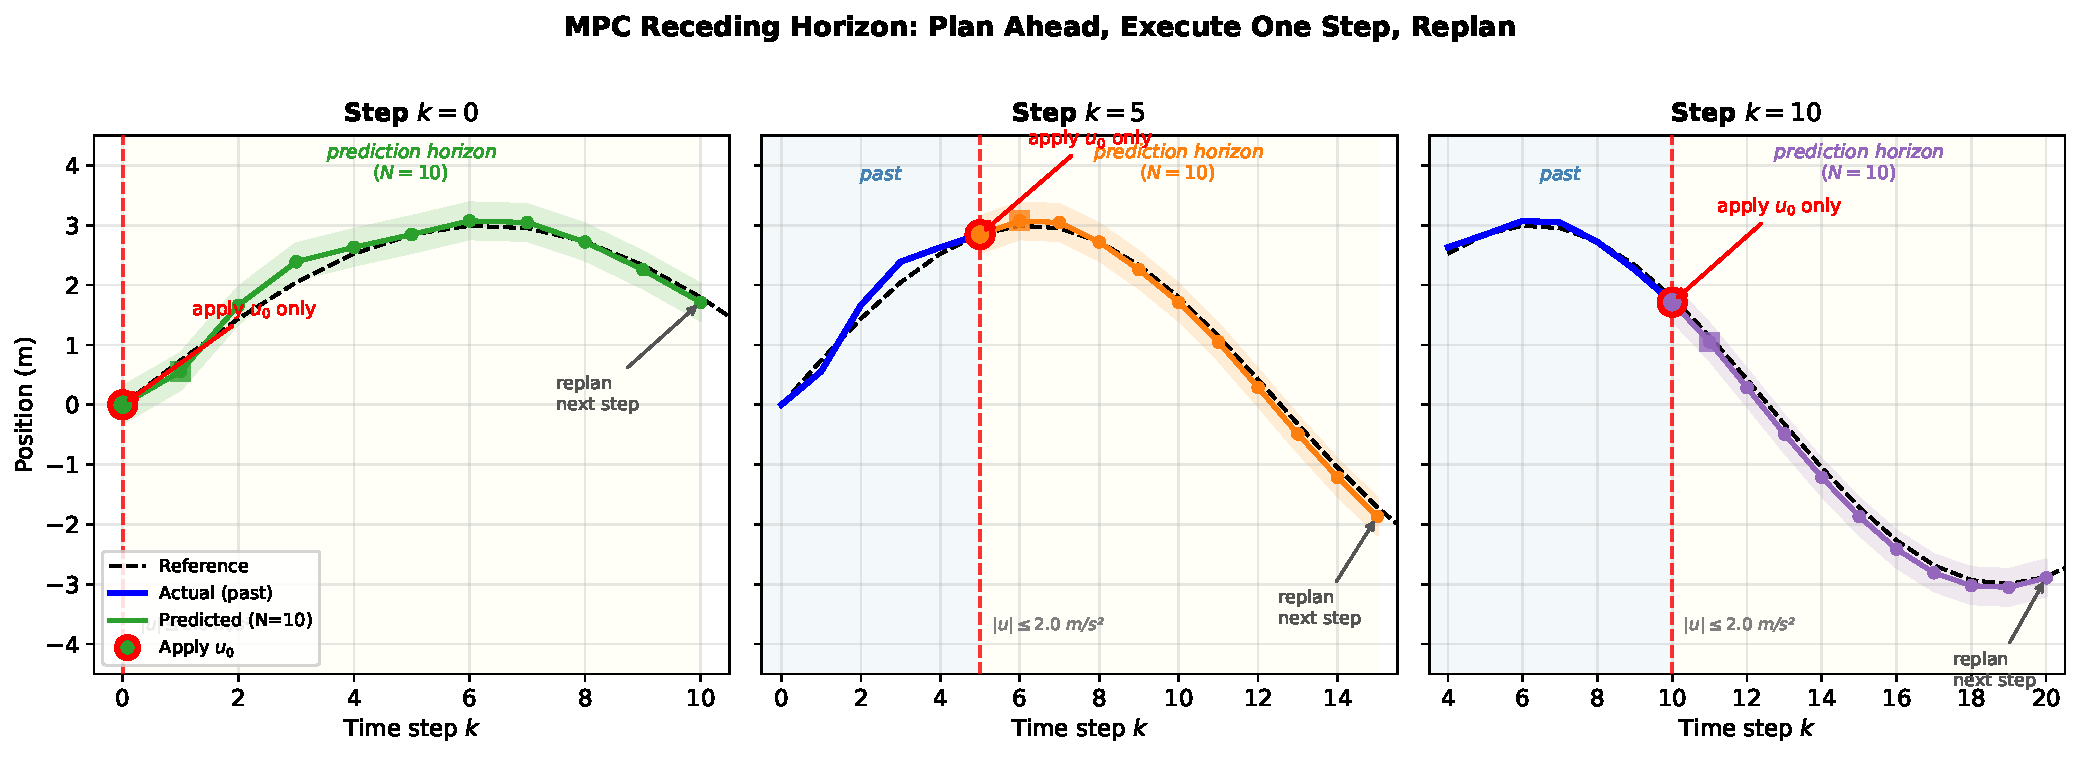
\includegraphics[width=\textwidth]{mpc_horizon.pdf}
\caption{MPC 滚动时域在位置跟踪问题上的示意图。在每个时间步，MPC 规划未来 $N=10$ 步的最优轨迹（绿色），但只施加\textbf{第一个}控制动作（圆圈标出）。然后重新测量、重新规划、反复循环。预测窗口随每步向前滑动——这种「向前规划、执行一步、再规划」的循环，正是 MPC 对模型误差和干扰具有鲁棒性的原因。}
\end{figure}

\subsubsection{TinyMPC：面向嵌入式系统的 Riccati 加速 MPC}

标准 MPC 在每个时间步都求解一个完整的二次规划（QP）。对于一个有 $n$ 个状态、$m$ 个输入、时域为 $N$ 的系统，这意味着求解一个有 $N(n+m)$ 个决策变量的问题——在笔记本电脑上可行，但对微控制器来说极为繁重。\textbf{TinyMPC}（Nguyen 等，2024）是一个突破性成果，它通过利用 Riccati 方程的结构，使 MPC 能够在资源受限的嵌入式系统（Teensy、STM32，甚至 Arduino）上运行。

\textbf{核心思路：} 对于无约束的线性 MPC，其解就是一个时变的 LQR——可以通过向后 Riccati 递推计算得到。TinyMPC 将这个 Riccati 递推\textbf{离线}预计算完成，然后用轻量的 ADMM（交替方向乘子法，Alternating Direction Method of Multipliers）循环\textbf{在线}处理约束。

\textbf{算法结构：}

\textit{第一步——离线预计算（一次性，或当模型改变时）：}

从终端代价 $P_N = Q_f$ 出发，向后运行 Riccati 递推，计算每步的最优反馈增益：
\begin{align}
S_k &= R + B_d^T P_{k+1} B_d \\
K_k &= S_k^{-1} B_d^T P_{k+1} A_d \\
P_k &= Q + A_d^T P_{k+1} A_d - A_d^T P_{k+1} B_d K_k
\end{align}

这给出 $N$ 个反馈增益矩阵 $K_0, K_1, \ldots, K_{N-1}$ 和 $N+1$ 个代价矩阵 $P_0, P_1, \ldots, P_N$。这些存储在内存中，\textit{不再重复计算}（除非模型或代价矩阵发生变化）。

\textit{第二步——在线求解（每个控制周期）：}

给定当前状态 $\mathbf{x}_0$：
\begin{enumerate}
    \item \textbf{前向展开：} 使用预计算的增益计算无约束最优轨迹：$\mathbf{u}_k = -K_k (\mathbf{x}_k - \mathbf{x}_k^{\text{ref}})$，然后 $\mathbf{x}_{k+1} = A_d \mathbf{x}_k + B_d \mathbf{u}_k$。
    \item \textbf{ADMM 投影：} 若任意 $\mathbf{u}_k$ 或 $\mathbf{x}_k$ 违反约束，运行几次 ADMM 迭代（通常 5--20 次），找到最近的可行解。每次 ADMM 迭代只需：
    \begin{itemize}[nosep]
        \item 一次类 Riccati 的向后遍历（使用\textit{预计算}的 $K_k$，因此代价低廉）。
        \item 一次投影步：$z_k = \text{clamp}(u_k + \lambda_k, u_{\min}, u_{\max})$——逐元素截断。
        \item 一次对偶更新：$\lambda_k \leftarrow \lambda_k + u_k - z_k$。
    \end{itemize}
    \item \textbf{施加第一个输入：} 将 $\mathbf{u}_0$ 发送给执行器。丢弃其余部分（滚动时域）。
\end{enumerate}

\textbf{为何速度如此之快：}
\begin{itemize}
    \item Riccati 递推（计算量最大的部分）已在\textbf{离线}完成。在线工作只是矩阵乘法和截断操作。
    \item 无需 QP 求解器库。在线无需矩阵分解。只需乘加和截断。
    \item 每次 ADMM 迭代的复杂度为 $O(N \cdot n^2)$——与时域成线性关系，与状态维度成二次关系。对于 4 状态系统、$N = 10$：每次迭代约 1600 次乘加。10 次迭代共 16000 次乘加——STM32F4 在 168 MHz 下可在 $< 100\,\mu$s 内完成。
    \item 内存占用：$N \times (n \times n + m \times n)$ 个浮点数用于预计算增益。对于 4 状态、2 输入、$N = 10$：约 240 个浮点数 = 960 字节。
\end{itemize}

\textbf{与标准基于 QP 的 MPC 对比：}

\begin{center}
\begin{tabular}{lcc}
\toprule
 & \textbf{标准 MPC（OSQP）} & \textbf{TinyMPC} \\
\midrule
在线计算 & 完整 QP 求解 & Riccati 展开 + ADMM \\
典型求解时间（STM32） & 1--10 ms & 50--200 $\mu$s \\
内存 & 数 KB（稀疏矩阵） & 小型系统 $<$ 1 KB \\
依赖项 & QP 求解器库 & 无（仅矩阵运算） \\
约束处理 & 精确（到容差） & 近似（ADMM） \\
热启动 & 可行 & 自然（用上一次解） \\
\bottomrule
\end{tabular}
\end{center}

\textbf{何时使用 TinyMPC：}
\begin{itemize}
    \item 需要在 RAM/CPU 有限的微控制器上运行 MPC。
    \item 模型是线性的（或可以在每步线性化用于非线性系统）。
    \item 对输入的硬约束很重要（电机电流限制、关节角度限制）。
    \item 时域较短到中等（$N \leq 30$）。
\end{itemize}

\textbf{何时不用 TinyMPC：}
\begin{itemize}
    \item 复杂非线性模型（在功能更强的计算机上使用 acados 或 CasADi）。
    \item 时域很长（$N > 50$）且有大量状态约束。
    \item 如果问题无约束——直接用 LQR，它更简单。
\end{itemize}

\textbf{参考：} TinyMPC 的完整论文和开源实现见 \texttt{tinympc.org}。C 实现不超过 1000 行，可在 ARM Cortex-M 微控制器上运行。附录中的 C++ 模块遵循同样的 Riccati + ADMM 结构。

\textbf{非线性系统怎么办？}线性 MPC 假设 $\mathbf{x}_{k+1} = A_d \mathbf{x}_k + B_d \mathbf{u}_k$，当工作范围较宽时就不够了。\textbf{非线性 MPC（NMPC）}用完整非线性动力学 $\mathbf{x}_{k+1} = f(\mathbf{x}_k, \mathbf{u}_k)$ 替代线性模型，将 QP 变为非线性规划（NLP）。我们在非线性控制章节中详细讨论 NMPC，并通过一个具体的轨迹跟踪实例将其与线性 MPC 做正面对比。

\subsection{基于状态空间的观测器设计}

LQR（以及所有状态反馈）都要求你知道全部状态。但实际中往往只能测到一部分。\textbf{观测器}（Observer，也叫估计器）的作用就是从能拿到的测量值里把完整状态"猜"出来。

\subsubsection{龙伯格观测器（Luenberger Observer）}

龙伯格观测器的思路很直接：复制一份系统模型，再加一个修正项，用测量误差把估计值往真实状态方向拽。

\begin{equation}
\dot{\hat{\mathbf{x}}} = A\hat{\mathbf{x}} + B\mathbf{u} + L(\mathbf{y} - C\hat{\mathbf{x}})
\end{equation}

其中：
\begin{itemize}[nosep]
    \item $\hat{\mathbf{x}}$ 是估计状态。
    \item $\mathbf{y} = C\mathbf{x}$ 是实际测量值。
    \item $L$ 是观测器增益矩阵（由我们设计）。
\end{itemize}

估计误差 $\mathbf{e} = \mathbf{x} - \hat{\mathbf{x}}$ 的演化方程为：
\begin{equation}
\dot{\mathbf{e}} = (A - LC)\mathbf{e}
\end{equation}

推导：将观测器方程 $\dot{\hat{\mathbf{x}}} = A\hat{\mathbf{x}} + B\mathbf{u} + L(\mathbf{y} - C\hat{\mathbf{x}})$ 从真实系统 $\dot{\mathbf{x}} = A\mathbf{x} + B\mathbf{u}$ 中减去。$B\mathbf{u}$ 项抵消，代入 $\mathbf{y} = C\mathbf{x}$ 得 $\dot{\mathbf{e}} = A\mathbf{e} - LC\mathbf{e} = (A - LC)\mathbf{e}$。

若选择 $L$ 使 $(A - LC)$ 的所有特征值都有负实部，估计误差将衰减到零。观测器「追上」真实状态。

\textbf{设计经验法则：} 将观测器的极点配置得比控制器极点快 2--5 倍。观测器的收敛速度应比控制器动作快，这样控制器始终有一个良好的状态估计。

\textbf{分离原理（Separation Principle）：} 你可以独立设计控制器增益 $K$ 和观测器增益 $L$。只要每个部分单独稳定，组合的控制器-观测器系统就是稳定的。这是一个优美的理论结果，极大地简化了设计过程。

\textbf{何时使用龙伯格观测器：} 当你的模型准确且噪声特性不很清楚时。它简单、确定性强、易于调试。

\subsubsection{深刻的对偶性：控制器与观测器互为镜像}

这是控制理论里最漂亮的结论之一。搞懂它，你对控制系统的理解会上一个台阶。下面把这种对称结构摆出来。

\textbf{控制器问题：} 给定系统 $\dot{\mathbf{x}} = A\mathbf{x} + B\mathbf{u}$，找到增益 $K$ 使得 $\mathbf{u} = -K\mathbf{x}$ 能让闭环系统 $\dot{\mathbf{x}} = (A - BK)\mathbf{x}$ 稳定且表现良好。

\textbf{观测器问题：} 给定系统 $\dot{\mathbf{x}} = A\mathbf{x} + B\mathbf{u}$，$\mathbf{y} = C\mathbf{x}$，找到增益 $L$ 使得估计误差 $\dot{\mathbf{e}} = (A - LC)\mathbf{e}$ 衰减到零。

现在并排对比两个闭环矩阵：

\begin{center}
\begin{tabular}{lcc}
\toprule
 & \textbf{控制器} & \textbf{观测器} \\
\midrule
闭环矩阵 & $A - BK$ & $A - LC$ \\
待设计的增益 & $K$ & $L$ \\
必要条件 & 可控性 $(A, B)$ & 可观性 $(A, C)$ \\
设计目标 & 配置 $A - BK$ 的特征值 & 配置 $A - LC$ 的特征值 \\
信息流向 & 输入 $\to$ 状态 & 测量 $\to$ 状态估计 \\
Riccati 方程 & $A^TP + PA - PBR^{-1}B^TP + Q = 0$ & $AP_o + P_oA^T - P_oC^TR_n^{-1}CP_o + Q_n = 0$ \\
\bottomrule
\end{tabular}
\end{center}

\textbf{数学对偶性：} 若将观测器 Riccati 方程转置，令 $A \to A^T$、$C^T \to B$、$Q_n \to Q$、$R_n \to R$，你会得到与控制器 Riccati 方程完全相同的形式。它们字面上是同一个方程，只是矩阵转置了。这意味着：

\begin{itemize}
    \item 任何设计控制器的算法都可以设计观测器（只需转置输入）。
    \item 若你能用 \texttt{place(A, B, poles)} 为控制器配置极点，就能用 \texttt{place(A', C', poles)'} 配置观测器极点——注意转置。
    \item LQR 控制器（来自控制 Riccati 的 $K$）有一个对偶：\textbf{卡尔曼滤波器（Kalman Filter）}（来自观测器 Riccati 的 $L$）。LQR 是最优控制器；卡尔曼是最优观测器。它们是对偶问题。
\end{itemize}

\textbf{打个比方：}控制器是\textit{扬声器}，观测器是\textit{麦克风}。扬声器（控制器）通过输入 $B$ 向系统注入能量，塑造状态轨迹。麦克风（观测器）通过输出 $C$ 监听系统，重建内部状况。可控性问的是："扬声器能覆盖房间的每个角落吗？"可观性问的是："麦克风能听到房间的每个角落吗？"同一个房间，对称的两个问题。

\textbf{实际价值：}你调状态反馈控制器时积累的直觉——极点越快响应越快但越怕噪声，极点越慢估计越稳但跟踪越慢——设计观测器时\textit{完全通用}。你在拧同一个旋钮，只不过拧的是镜子的另一面。

\subsubsection{卡尔曼滤波器（Kalman Filter）}

卡尔曼滤波器是线性高斯系统下的最优观测器，可以看作龙伯格观测器的"概率升级版"——不用手动配极点，而是根据噪声统计特性自动算出最优增益 $L$。

\textbf{带噪声的系统模型：}
\begin{align}
\mathbf{x}[k+1] &= A_d \mathbf{x}[k] + B_d \mathbf{u}[k] + \mathbf{w}[k], \quad \mathbf{w} \sim \mathcal{N}(0, Q_n) \\
\mathbf{y}[k] &= C \mathbf{x}[k] + \mathbf{v}[k], \quad \mathbf{v} \sim \mathcal{N}(0, R_n)
\end{align}

其中 $\mathbf{w}$ 是过程噪声（模型不确定性），$\mathbf{v}$ 是测量噪声。$Q_n$ 和 $R_n$ 是它们各自的协方差矩阵。

\textbf{卡尔曼滤波器算法（离散时间）：}

\textit{预测（Predict）：}
\begin{align}
\hat{\mathbf{x}}[k|k-1] &= A_d \hat{\mathbf{x}}[k-1|k-1] + B_d \mathbf{u}[k-1] \\
P[k|k-1] &= A_d P[k-1|k-1] A_d^T + Q_n
\end{align}

\textit{更新（Update）：}
\begin{align}
K_k &= P[k|k-1] C^T (C P[k|k-1] C^T + R_n)^{-1} \\
\hat{\mathbf{x}}[k|k] &= \hat{\mathbf{x}}[k|k-1] + K_k (\mathbf{y}[k] - C \hat{\mathbf{x}}[k|k-1]) \\
P[k|k] &= (I - K_k C) P[k|k-1]
\end{align}

\textbf{直觉：}卡尔曼增益 $K_k$ 在模型预测和测量之间自动分配信任度：
\begin{itemize}
    \item 若过程噪声大（$Q_n$ 大）而测量噪声小（$R_n$ 小），滤波器更信任测量值。
    \item 若测量噪声大而过程噪声小，滤波器更信任模型。
\end{itemize}

\textbf{卡尔曼滤波器调参} 归结于选择 $Q_n$ 和 $R_n$：
\begin{itemize}
    \item $R_n$ 通常可以直接测量（在系统静止时记录传感器数据，计算方差）。
    \item $Q_n$ 更难确定——它代表模型不确定性。从较小的值开始，若滤波器太迟钝（跟踪不够快），则增大。
    \item 一个常用技巧：将 $Q_n$ 和 $R_n$ 当作调节旋钮。增大 $Q_n / R_n$ 的比值以获得更快的跟踪（但噪声更多）。减小以获得更平滑的估计（但有更多滞后）。听起来很熟悉？这与低通滤波器截止频率的权衡相同，只是用概率语言表达。
\end{itemize}

\textbf{为什么机器人圈子到处都是卡尔曼：}
\begin{itemize}
    \item \textbf{传感器融合：} 将 IMU、编码器和视觉数据融合成一个连贯的状态估计。
    \item \textbf{速度估计：} 从有噪声的位置测量中获得平滑的速度，而不使用纯微分器。
    \item \textbf{在明确意义下最优：} 对于线性高斯系统，它最小化均方估计误差。
\end{itemize}

\textbf{实用说明：} 卡尔曼滤波器每步需要一次矩阵求逆（$K_k$ 的计算）。对于小状态维度（$n \leq 6$），这微不足道。对于更大的系统，使用高效实现（如 Cholesky 分解）。在 STM32F4 上，一个 6 状态的 EKF 可以在 1 kHz 下舒适地运行。

\subsubsection{扩展卡尔曼滤波器（EKF）}

标准卡尔曼滤波器假设线性动力学和线性测量。但真实机器人系统是\textbf{非线性的}：欧拉角和角速度之间是三角函数关系，加速度计的测量模型跟倾斜角的正弦余弦有关，等等。

\textbf{扩展卡尔曼滤波器（EKF）}的处理方式很粗暴也很有效：每一步都在当前估计值附近把系统\textit{线性化}，当成线性的来跑标准卡尔曼，然后在新估计值处重新线性化。

\textbf{非线性系统模型：}
\begin{align}
\mathbf{x}_{k+1} &= f(\mathbf{x}_k, \mathbf{u}_k) + \mathbf{w}_k \quad \text{（非线性动力学）} \\
\mathbf{y}_k &= h(\mathbf{x}_k) + \mathbf{v}_k \quad \text{（非线性测量）}
\end{align}

\textbf{雅可比矩阵——它是什么，为什么需要它。}\;卡尔曼滤波的协方差传播公式（$P_{k|k-1} = A P_{k-1|k-1} A^T + Q$）需要一个\emph{矩阵} $A$。但非线性系统没有单一的 $A$——$f$ 的"斜率"处处不同。解决办法就是用\textbf{雅可比矩阵（Jacobian）}，它是导数在多变量情况下的自然推广。

回忆高数：对于标量函数 $y = f(x)$，导数 $f'(x_0)$ 给出了在 $x_0$ 附近的最佳线性近似：$f(x) \approx f(x_0) + f'(x_0)(x - x_0)$。雅可比矩阵对\emph{多元向量值}函数做同样的事。若 $\mathbf{f}: \mathbb{R}^n \to \mathbb{R}^m$，雅可比矩阵是所有偏导数组成的 $m \times n$ 矩阵：
\[
F = \frac{\partial \mathbf{f}}{\partial \mathbf{x}} = \begin{bmatrix}
\frac{\partial f_1}{\partial x_1} & \cdots & \frac{\partial f_1}{\partial x_n} \\
\vdots & \ddots & \vdots \\
\frac{\partial f_m}{\partial x_1} & \cdots & \frac{\partial f_m}{\partial x_n}
\end{bmatrix}.
\]
每一行告诉你某个输出分量相对于所有输入的变化率。在特定点 $\mathbf{x}_0$ 处求值后，雅可比矩阵给出最佳局部线性近似：$\mathbf{f}(\mathbf{x}) \approx \mathbf{f}(\mathbf{x}_0) + F(\mathbf{x} - \mathbf{x}_0)$——这正是 EKF"假装系统局部线性"所需要的那一步。

\textbf{EKF 算法：}

\textit{预测：}
\begin{align}
\hat{\mathbf{x}}_{k|k-1} &= f(\hat{\mathbf{x}}_{k-1|k-1}, \mathbf{u}_{k-1}) \\
F_k &= \left.\frac{\partial f}{\partial \mathbf{x}}\right|_{\hat{\mathbf{x}}_{k-1|k-1}} \quad \text{（动力学雅可比矩阵）} \\
P_{k|k-1} &= F_k P_{k-1|k-1} F_k^T + Q
\end{align}

\textit{更新：}
\begin{align}
H_k &= \left.\frac{\partial h}{\partial \mathbf{x}}\right|_{\hat{\mathbf{x}}_{k|k-1}} \quad \text{（测量雅可比矩阵）} \\
K_k &= P_{k|k-1} H_k^T (H_k P_{k|k-1} H_k^T + R)^{-1} \\
\hat{\mathbf{x}}_{k|k} &= \hat{\mathbf{x}}_{k|k-1} + K_k \left(\mathbf{y}_k - h(\hat{\mathbf{x}}_{k|k-1})\right) \\
P_{k|k} &= (I - K_k H_k) P_{k|k-1}
\end{align}

\textbf{与标准卡尔曼滤波器的唯一区别：}
\begin{enumerate}
    \item 预测使用\textit{非线性}函数 $f(\cdot)$ 代替矩阵 $A$。
    \item 测量残差使用\textit{非线性}函数 $h(\cdot)$ 代替矩阵 $C$。
    \item 协方差传播使用（在当前估计处求值的）\textit{雅可比矩阵} $F_k$ 和 $H_k$，代替常数矩阵 $A$ 和 $C$。
\end{enumerate}

其余所有部分——卡尔曼增益公式、协方差更新、预测-更新循环——都\textit{完全相同}。

\vspace{0.5em}
\begin{mdframed}[linewidth=1pt, innertopmargin=10pt, innerbottommargin=10pt]
\textbf{案例研究：基于 EKF 的 6-DOF IMU 位姿估计}

\vspace{0.3em}
比赛机器人里最常见的 EKF 应用：用六轴 IMU（三轴加速度计 + 三轴陀螺仪）估计机器人的三维姿态（横滚、俯仰、偏航）。

\textbf{状态向量：} $\mathbf{x} = [\phi, \theta, \psi, b_x, b_y, b_z]^T$
\begin{itemize}[nosep]
    \item $\phi$：横滚，$\theta$：俯仰，$\psi$：偏航（弧度制欧拉角）
    \item $b_x, b_y, b_z$：陀螺仪偏差（rad/s）——EKF 自动估计这些偏差
\end{itemize}

\textbf{动力学模型 $f(\mathbf{x}, \mathbf{u})$：} 经过偏差补偿后的陀螺仪角速度通过运动学方程驱动欧拉角：
\begin{align}
\omega_x &= \text{gyro}_x - b_x, \quad \omega_y = \text{gyro}_y - b_y, \quad \omega_z = \text{gyro}_z - b_z \\[3pt]
\dot{\phi} &= \omega_x + \sin\phi \tan\theta \cdot \omega_y + \cos\phi \tan\theta \cdot \omega_z \\
\dot{\theta} &= \cos\phi \cdot \omega_y - \sin\phi \cdot \omega_z \\
\dot{\psi} &= \frac{\sin\phi}{\cos\theta} \cdot \omega_y + \frac{\cos\phi}{\cos\theta} \cdot \omega_z \\[3pt]
\dot{b}_x &= 0, \quad \dot{b}_y = 0, \quad \dot{b}_z = 0 \quad \text{（偏差建模为随机游走）}
\end{align}

雅可比矩阵 $F = \frac{\partial f}{\partial \mathbf{x}}$ 是一个含三角函数元素的 $6 \times 6$ 矩阵，必须在每个时间步重新计算（这就是「扩展」的部分）。

\textbf{测量模型 $h(\mathbf{x})$：} 加速度计测量重力方向，从而给出横滚和俯仰（但\textbf{不能}给出偏航）：
\begin{align}
h(\mathbf{x}) = \begin{bmatrix} \phi \\ \theta \end{bmatrix} = \begin{bmatrix} \arctan2(a_y, a_z) \\ \arctan2(-a_x, \sqrt{a_y^2 + a_z^2}) \end{bmatrix}
\end{align}

雅可比矩阵很简单：$H = \begin{bmatrix} 1 & 0 & 0 & 0 & 0 & 0 \\ 0 & 1 & 0 & 0 & 0 & 0 \end{bmatrix}$。

\textbf{关键设计决策：}
\begin{itemize}[nosep]
    \item \textbf{偏航不可观测}——单靠六轴 IMU，重力无法告诉你哪个方向是北。偏航完全依赖陀螺仪。要纠正偏航漂移，需要添加磁力计（九轴 IMU）或外部航向参考。
    \item \textbf{$Q$ 矩阵调参：} 角度对应的对角元素（$Q_{00}, Q_{11}, Q_{22}$）代表每步陀螺仪积分的漂移程度。越大 = 越不信任陀螺仪。偏差项（$Q_{33}, Q_{44}, Q_{55}$）代表偏差随机游走速率——通常很小（$10^{-4}$ 到 $10^{-6}$）。
    \item \textbf{$R$ 矩阵调参：} 代表加速度计噪声。在振动或线性加速期间，加速度计读数会被污染。在高加速度机动时增大 $R$（自适应 EKF），避免信任不良的加速度计数据。
    \item \textbf{万向锁（Gimbal Lock）：} 当俯仰角 $= \pm 90$\textdegree{} 时，运动学方程中的 $\tan\theta$ 和 $1/\cos\theta$ 项趋于无穷大。对于可能倾斜超过 $\pm 60$\textdegree{} 的机器人，使用\textbf{四元数表示}代替欧拉角（EKF 结构相同，状态参数化不同）。
\end{itemize}
\end{mdframed}

\begin{figure}[H]
\centering
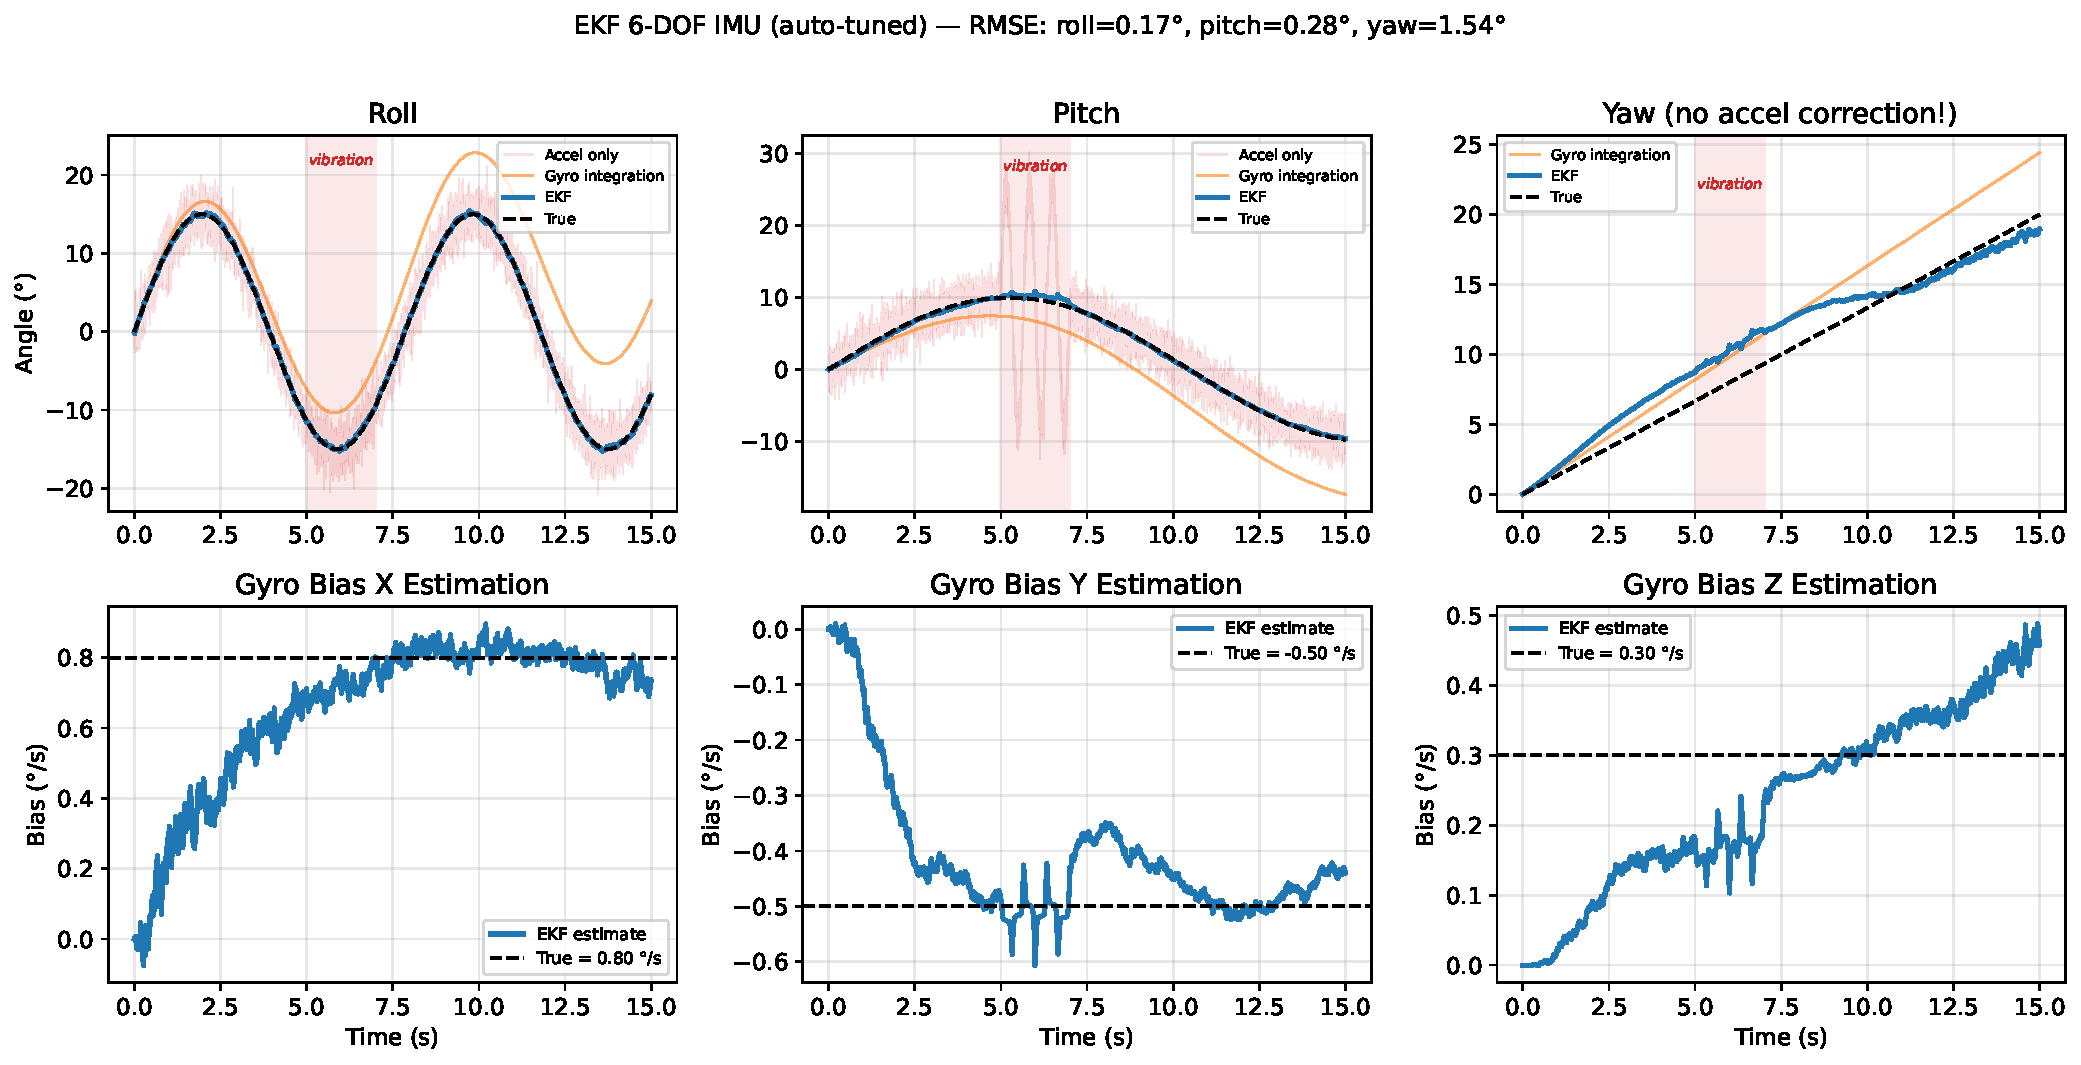
\includegraphics[width=\textwidth]{ekf_imu_6dof.pdf}
\caption{EKF 6-DOF IMU 位姿估计，配合自动调参的连续自适应 $R$。使用平滑指数缩放 $R = R_\text{base} \cdot (1 + \alpha \, e^{\beta \cdot \Delta a})$，横滚和俯仰分别有独立的 $R_\text{base}$，并加入俯仰专用的 $x$ 轴加速度偏差检测。参数通过离线网格搜索确定，最小化加权 RMSE。顶行：横滚（RMSE 0.17\textdegree）、俯仰（0.28\textdegree）、偏航（1.54\textdegree）。振动期间（$t = 5$--$7$s，阴影区域），自适应 $R$ 指数增大，拒绝被污染的加速度计数据。偏航漂移仅靠偏差估计得以限制（无航向参考）。底行：陀螺仪偏差平稳收敛至真实值。}
\end{figure}

\textbf{EKF 之外：} 当状态不确定性较大或非线性较强时，EKF 的线性化可能不准确。替代方案：
\begin{itemize}
    \item \textbf{无迹卡尔曼滤波器（Unscented Kalman Filter，UKF）：} 不进行线性化，而是将「sigma 点」（一组精心选取的样本状态）通过非线性函数传播。对高度非线性系统比 EKF 更准确，但略微昂贵（每步需要 $2n+1$ 次函数求值，$n$ 为状态维度）。
    \item \textbf{误差状态卡尔曼滤波器（Error-State Kalman Filter，ESKF）：} 估计围绕名义轨迹的\textit{小误差}，而不是完整状态。在基于 IMU 的系统中很流行，因为误差状态保持较小（线性化准确），且避免了四元数奇异性。这是大多数生产级 IMU 融合库内部所使用的方法。
    \item \textbf{互补滤波器（Complementary Filter）：} 对于计算资源极其有限的简单横滚/俯仰估计，互补滤波器（第 2 节）仍然是一个可行的单行代码替代方案。
\end{itemize}

\subsubsection{基于四元数的 EKF：避免万向锁}

前面的欧拉角 EKF 在俯仰角 $\pm 60$\textdegree{} 以内跑得挺好。但俯仰角接近 $\pm 90$\textdegree{} 时，运动学方程直接炸了：$\tan\theta \to \infty$，$1/\cos\theta \to \infty$。这就是\textbf{万向锁（Gimbal Lock）}——数学上的奇异性，不是物理上的。机器人好好的，是你的公式坏了。

解决方法是用\textbf{单位四元数} $\mathbf{q} = \begin{bmatrix} q_w & q_x & q_y & q_z \end{bmatrix}^T$ 代替欧拉角来表示姿态。四元数没有奇异性，结构紧凑（4 个数，相比旋转矩阵的 9 个），并且可以高效地合成旋转。

\textbf{状态向量：} $\mathbf{x} = \begin{bmatrix} \mathbf{q}^T & \boldsymbol{\beta}^T \end{bmatrix}^T \in \mathbb{R}^7$，其中 $\boldsymbol{\beta} = \begin{bmatrix} \beta_x & \beta_y & \beta_z \end{bmatrix}^T$ 为陀螺仪偏差。

\textbf{预测步骤：} 给定陀螺仪测量值 $\boldsymbol{\omega}_m$，经偏差修正后的角速度为 $\boldsymbol{\omega} = \boldsymbol{\omega}_m - \boldsymbol{\beta}$。四元数运动学方程为：
\begin{equation}
\dot{\mathbf{q}} = \frac{1}{2}\mathbf{q} \otimes \begin{bmatrix} 0 \\ \boldsymbol{\omega} \end{bmatrix}
= \frac{1}{2}\Omega(\boldsymbol{\omega})\,\mathbf{q}
\end{equation}

其中 $\otimes$ 是四元数乘法，$\Omega(\boldsymbol{\omega})$ 是 $4\times 4$ 斜对称矩阵：
\begin{equation}
\Omega(\boldsymbol{\omega}) = \begin{bmatrix}
0 & -\omega_x & -\omega_y & -\omega_z \\
\omega_x & 0 & \omega_z & -\omega_y \\
\omega_y & -\omega_z & 0 & \omega_x \\
\omega_z & \omega_y & -\omega_x & 0
\end{bmatrix}
\end{equation}

离散时间预测（一阶近似）：
\begin{equation}
\mathbf{q}_{k+1} = \left(I + \frac{\Delta t}{2}\Omega(\boldsymbol{\omega}_k)\right)\mathbf{q}_k, \qquad
\boldsymbol{\beta}_{k+1} = \boldsymbol{\beta}_k
\end{equation}

预测后，将 $\mathbf{q}$ \textbf{归一化}为单位长度：$\mathbf{q} \leftarrow \mathbf{q}/\|\mathbf{q}\|$。

\textbf{测量模型：} 加速度计测量体坐标系中的重力方向。给定四元数 $\mathbf{q}$，体坐标系中预测的重力方向为：
\begin{equation}
\mathbf{g}_{\text{pred}} = R(\mathbf{q})^T \begin{bmatrix} 0 \\ 0 \\ g \end{bmatrix}
= g\begin{bmatrix}
2(q_x q_z - q_w q_y) \\
2(q_y q_z + q_w q_x) \\
q_w^2 - q_x^2 - q_y^2 + q_z^2
\end{bmatrix}
\end{equation}

测量雅可比矩阵 $H = \partial \mathbf{g}_{\text{pred}} / \partial \mathbf{x}$ 是一个 $3\times 7$ 矩阵（3 个加速度计分量，4 个四元数 + 3 个偏差状态）。偏差列为零，因为加速度计读数与陀螺仪偏差不直接相关。

\textbf{更新步骤：} 标准 EKF 更新照常进行。残差为 $\boldsymbol{\nu} = \mathbf{a}_{\text{meas}} - \mathbf{g}_{\text{pred}}$，更新后再次将 $\mathbf{q}$ 归一化。

\begin{mdframed}[linewidth=1pt, innertopmargin=10pt, innerbottommargin=10pt]
\textbf{欧拉角与四元数：何时用哪个}

\vspace{0.3em}
\begin{itemize}[nosep]
    \item \textbf{欧拉角}：若你的机器人在俯仰角 $\pm 60$\textdegree{} 范围内工作（地面车辆、大多数炮塔、正常飞行的大多数无人机），欧拉角完全可行。数学更直观，也更容易调试。
    \item \textbf{四元数}：对于可能翻转、翻滚或垂直指向的机器人（特技无人机、水下 ROV、机械臂腕部附近的奇异点），四元数是必要的。
    \item \textbf{提示：} 你可以在内部使用四元数进行所有计算，仅在显示和人类可读的日志中转换为欧拉角：$\phi = \text{atan2}(2(q_w q_x + q_y q_z),\; 1 - 2(q_x^2 + q_y^2))$，等等。
    \item \textbf{误差状态方法（ESKF）} 避免在 EKF 状态中直接使用 4 元素四元数。它改为估计 3 元素旋转误差 $\delta\boldsymbol{\theta}$，并在每次更新后将其应用到四元数上。这使协方差矩阵 $P$ 保持 $6\times 6$ 而非 $7\times 7$，并避免了单位范数约束问题。大多数生产级 IMU 库（如 PX4 的 EKF2、VINS-Mono）内部使用 ESKF。
\end{itemize}
\end{mdframed}

\subsubsection{自适应 EKF（Adaptive EKF）：在线自动调整 \texorpdfstring{$Q$}{Q} 和 \texorpdfstring{$R$}{R}}

EKF 效果好不好，很大程度上取决于噪声协方差 $Q$（过程噪声）和 $R$（测量噪声）。实际中这两个矩阵通常靠手调——一个磨人的试错过程。更麻烦的是，真实噪声在运行中\textit{会变}：装在振动底盘上的 IMU 和静止时的噪声特性根本不一回事。固定的 $Q$、$R$ 应付不了这种情况。

\textbf{自适应 EKF（Adaptive EKF）}方法能够\textit{在线}估计或调整 $Q$ 和 $R$，自动进行。以下是几种方法，从简单到复杂。

\textbf{方法一：基于残差的自适应估计（Innovation-Based Adaptive Estimation，IAE）}

最简单也最实用的一种方法。核心思路：\textbf{残差序列} $\boldsymbol{\nu}_k = \mathbf{y}_k - h(\hat{\mathbf{x}}_{k|k-1})$（测量值减去预测值）里就藏着 $Q$ 和 $R$ 到底对不对的信息。

\textit{判断依据：}滤波器调对了的话，残差应该是均值为零的白噪声，协方差 $S_k = H_k P_{k|k-1} H_k^T + R$。残差老是比预期大？要么 $Q$ 太小（太信模型了），要么 $R$ 太小（太信传感器了）。

\textbf{算法：} 使用最近 $N_w$ 个残差的滑动窗口估计实际残差协方差：
\begin{equation}
\hat{S}_k = \frac{1}{N_w} \sum_{j=k-N_w+1}^{k} \boldsymbol{\nu}_j \boldsymbol{\nu}_j^T
\end{equation}

然后更新 $R$ 使其匹配：
\begin{equation}
\hat{R}_k = \hat{S}_k - H_k P_{k|k-1} H_k^T
\end{equation}

若 $\hat{R}_k$ 出现负特征值（在 $N_w$ 较小时可能发生），将其截断到最小值。典型窗口大小：$N_w = 20$--$100$ 个样本。

\textbf{代码：}
\begin{verbatim}
    // After computing innovation nu = z - h(x_pred):
    // Accumulate outer product in sliding window
    innov_buffer[buf_idx] = nu;
    buf_idx = (buf_idx + 1) % N_WINDOW;

    if (samples_seen >= N_WINDOW) {
        // Estimate innovation covariance
        Mat<NZ,NZ> S_hat = Mat<NZ,NZ>::zeros();
        for (int j = 0; j < N_WINDOW; j++) {
            S_hat = S_hat + innov_buffer[j] * innov_buffer[j].T();
        }
        S_hat = S_hat * (1.0f / N_WINDOW);

        // Adapt R
        R = S_hat - H * P_pred * H.T();
        // Clamp diagonal to minimum (prevent negative/zero variance)
        for (int i = 0; i < NZ; i++)
            if (R(i,i) < R_min) R(i,i) = R_min;
    }
\end{verbatim}

\textbf{方法二：基于状态残差的 $Q$ 自适应}

IAE 方法用于自适应 $R$，而过程噪声 $Q$ 可以使用\textbf{状态残差}（预测状态与更新状态之差）来自适应：
\begin{equation}
\hat{Q}_k = \frac{1}{N_w} \sum_{j} (K_j \boldsymbol{\nu}_j)(K_j \boldsymbol{\nu}_j)^T + P_{k|k} - F_k P_{k-1|k-1} F_k^T
\end{equation}

这比 IAE 更复杂，数值稳定性也更差。在实践中，许多系统只自适应 $R$ 而保持 $Q$ 固定，因为 $R$ 变化更大（传感器噪声随环境变化），而 $Q$ 主要由模型不确定性决定（更为恒定）。

\textbf{方法三：衰减记忆（指数遗忘）}

最简单的「自适应」技巧：将预测协方差乘以\textbf{遗忘因子} $\alpha > 1$：
\begin{equation}
P_{k|k-1} = \alpha \cdot (F_k P_{k-1|k-1} F_k^T + Q)
\end{equation}

这在每步人为地增大不确定性，使滤波器「忘记」旧数据，更信任新测量值。这等效于在不显式改变 $Q$ 的情况下让 $Q$ 变大。

\begin{itemize}
    \item $\alpha = 1.0$：标准 EKF（不遗忘）。
    \item $\alpha = 1.01$--$1.05$：轻度自适应——滤波器对突然变化反应更快。
    \item $\alpha > 1.1$：非常激进——滤波器几乎忽略模型，跟着测量值走。仅在已知扰动期间使用。
\end{itemize}

\textbf{何时使用：} 当你预期会有偶发的突然模型变化时（例如，机械臂拾取了未知负载——惯性瞬间改变）。衰减记忆防止滤波器「锁定」在过时的动力学上。

\textbf{代码（在标准 EKF 中增加一行）：}
\begin{verbatim}
    P_pred = F * P * F.T() + Q;
    P_pred = P_pred * alpha;   // <-- fading memory, alpha = 1.01
\end{verbatim}

\textbf{方法四：多模式自适应 EKF（适用于 IMU）}

对于比赛机器人，最实用的方法是简单的\textbf{模式切换}策略，而不是连续自适应：

\begin{verbatim}
    // Compute acceleration magnitude
    float accel_mag = sqrt(ax*ax + ay*ay + az*az);
    float accel_err = fabs(accel_mag - 9.81f);

    if (accel_err < 0.5f) {
        // Stationary or slow motion: trust accelerometer
        ekf.R(0,0) = 0.05f;  ekf.R(1,1) = 0.05f;
    } else if (accel_err < 2.0f) {
        // Moderate motion: reduce trust
        ekf.R(0,0) = 0.5f;   ekf.R(1,1) = 0.5f;
    } else {
        // High acceleration / vibration: mostly ignore accelerometer
        ekf.R(0,0) = 10.0f;  ekf.R(1,1) = 10.0f;
    }
\end{verbatim}

\textbf{逻辑：} 当 $|\mathbf{a}| \approx g$（9.81 m/s$^2$）时，机器人没有线性加速度，加速度计确实在测量重力——信任它（$R$ 小）。当 $|\mathbf{a}|$ 偏离 $g$ 时，存在线性加速度或振动污染读数——不信任它（$R$ 大）。

数学上不优雅？无所谓。实战中\textbf{极其好使}。不少冠军机器人用的就是这套。鲁棒、好调（就三个阈值），计算量几乎为零。

\textbf{总结：用哪种方法？}

\begin{center}
\begin{tabular}{llll}
\toprule
\textbf{方法} & \textbf{自适应对象} & \textbf{复杂度} & \textbf{最适用场景} \\
\midrule
多模式切换 & $R$（离散） & 极简 & 移动机器人上的 IMU \\
衰减记忆 & 等效 $Q$ & 一行代码 & 突发模型变化 \\
IAE（基于残差） & $R$（连续） & 中等 & 传感器噪声变化 \\
基于状态残差 & $Q$ 和 $R$ & 高 & 科研/离线场合 \\
\bottomrule
\end{tabular}
\end{center}

\textbf{一句警告：} 若实现不当，自适应方法可能使滤波器\textit{发散}。务必将自适应后的 $Q$ 和 $R$ 截断到合理范围，使用最小窗口大小（$N_w \geq 20$），并在部署到硬件之前在记录的数据上进行验证。

\subsubsection{龙伯格观测器与卡尔曼滤波器：全面对比}

两种观测器都学了，放在一起比一下，看看什么场景用哪个。

\begin{center}
\begin{tabular}{p{3.5cm}p{5.5cm}p{5.5cm}}
\toprule
\textbf{方面} & \textbf{龙伯格观测器} & \textbf{卡尔曼滤波器} \\
\midrule
\textbf{设计输入} & 期望极点位置（你来选择） & 噪声协方差 $Q_n$、$R_n$（来自物理或调参） \\
\textbf{增益计算} & 一次性极点配置 & 递推（每步更新 $P$ 和 $K_k$）或稳态 \\
\textbf{最优性} & 非最优——你选择「合理」的极点 & 最优（对线性高斯系统最小化均方误差） \\
\textbf{噪声处理} & 无显式噪声模型——增益固定 & 显式建模过程噪声和测量噪声 \\
\textbf{自适应性} & 增益 $L$ 固定——在所有条件下相同 & 增益 $K_k$ 随不确定性 $P$ 的演化而自适应 \\
\textbf{计算代价} & 极低（仅矩阵乘法） & 较高（每步矩阵乘法 + 求逆） \\
\textbf{调参难度} & 中等（选择极点位置） & 中等（选择 $Q_n$、$R_n$） \\
\textbf{置信度输出} & 无 & $P$ 矩阵告诉你估计的置信程度 \\
\textbf{传感器融合} & 可行但需手动 & 自然——只需扩展 $C$ 矩阵 \\
\bottomrule
\end{tabular}
\end{center}

\textbf{它们之间的深层联系：}到了稳态（$k \to \infty$），卡尔曼增益 $K_k$ 收敛到常数 $K_\infty$。这时候卡尔曼滤波器\textit{就是}一个龙伯格观测器，取 $L = K_\infty$。差别在于：卡尔曼是从噪声统计特性里\textit{最优地算出}这个 $L$ 的，而龙伯格需要你凭直觉或极点配置来选。

再深挖一层：稳态卡尔曼增益 $K_\infty$ 是观测器 Riccati 方程的解——恰好是 LQR 那个控制器 Riccati 方程的对偶。对称性到此闭合：

\begin{center}
\begin{tabular}{lcc}
\toprule
 & \textbf{控制（输入）侧} & \textbf{估计（输出）侧} \\
\midrule
手动设计 & 配置 $K$ 的极点 & 龙伯格：配置 $L$ 的极点 \\
最优设计 & LQR：最小化 $\int (\mathbf{x}^TQ\mathbf{x} + \mathbf{u}^TR\mathbf{u})\,dt$ & 卡尔曼：最小化 $E[\|\mathbf{x} - \hat{\mathbf{x}}\|^2]$ \\
Riccati 变量 & $P$（控制代价函数） & $P$（估计不确定性） \\
调参旋钮 & $Q$ 对比 $R$（状态惩罚对比控制代价） & $Q_n$ 对比 $R_n$（模型信任对比传感器信任） \\
\bottomrule
\end{tabular}
\end{center}

\subsubsection{LQG（线性二次高斯控制器）}

LQR（最优控制器）和卡尔曼滤波器（最优观测器）都有了，把它们拼在一起就是 LQG。\textbf{LQG（Linear Quadratic Gaussian，线性二次型高斯控制器）}就是将两者结合的结果：LQR负责控制，卡尔曼滤波器负责估计，而分离原理（separation principle）保证了这种组合的稳定性。

\textbf{LQG架构：}
\begin{align}
\text{卡尔曼滤波器：} \quad \dot{\hat{\mathbf{x}}} &= A\hat{\mathbf{x}} + B\mathbf{u} + L(\mathbf{y} - C\hat{\mathbf{x}}) \\
\text{LQR控制器：} \quad \mathbf{u} &= -K\hat{\mathbf{x}}
\end{align}

其中 $K$ 来自控制Riccati方程（最小化状态代价），$L$ 来自估计Riccati方程（最小化估计误差）。控制器从不接触真实状态——它作用于卡尔曼估计值。

\textbf{为什么LQG在MIMO/噪声系统中优于PID：}
\begin{enumerate}
    \item \textbf{最优噪声处理：}PID通过微分项放大噪声。LQG的卡尔曼滤波器提供最小方差状态估计——为控制器提供尽可能干净的信号。
    \item \textbf{天然适合MIMO：}PID本质上是SISO的。对于4状态平衡机器人，PID需要层叠的多个回路和手工调整的交叉耦合。LQG用一个 $K$ 矩阵处理所有状态。
    \item \textbf{状态估计：}PID无法估计未测量的状态。LQG的卡尔曼滤波器可从部分测量（例如仅位置传感器）重建完整状态（包括速度）。
    \item \textbf{系统化整定：}PID每个回路有3个旋钮。LQG有 $Q$、$R$（控制代价）和 $Q_n$、$R_n$（噪声模型）——物理含义明确的矩阵。
\end{enumerate}

\textbf{LQG的鲁棒性警告：}纯LQR具有保证的稳定裕度（增益裕度 $\geq$ 6 dB，相位裕度 $\geq$ 60°）。当你加入卡尔曼滤波器构成LQG时，这些保证\textit{消失了}。LQG控制器可以有任意小的稳定裕度。这就是著名的\textbf{Doyle反例}（1978年）——它推动了 $H_\infty$ 鲁棒控制的发展。

\textbf{实践含义：}当模型准确且噪声特性明确时，LQG效果良好。若存在显著的模型不确定性（未知摩擦、变化载荷），可考虑：
\begin{itemize}
    \item \textbf{LQG/LTR（回路传递恢复，Loop Transfer Recovery）：}修改卡尔曼滤波器整定，在被控对象输入处恢复LQR的鲁棒性裕度。
    \item \textbf{$H_\infty$ 控制：}针对最坏情况的模型不确定性进行设计，而非平均噪声。
    \item \textbf{实用做法：}在 $\pm 30\%$ 参数变化的仿真中验证LQG。如果保持稳定，通常足够在比赛中使用。
\end{itemize}

\begin{figure}[H]
\centering
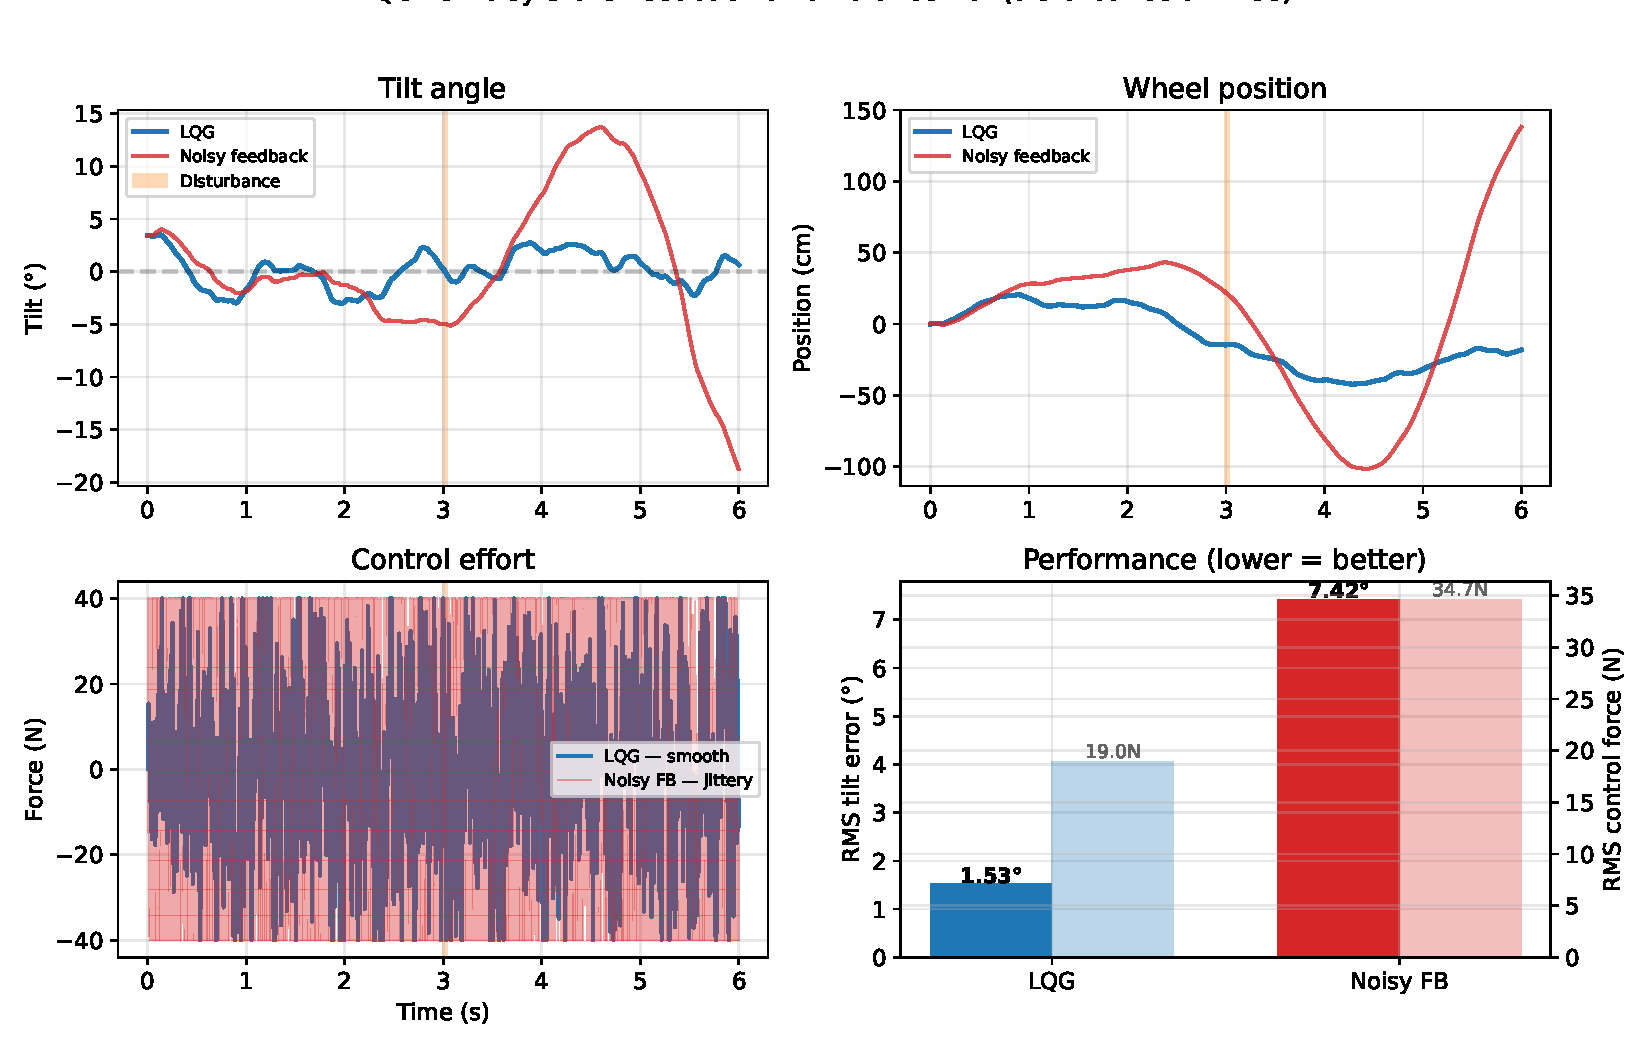
\includegraphics[width=\textwidth]{lqg_comparison.pdf}
\caption{LQG（蓝色）与直接带噪反馈（红色）在平衡机器人上的对比（$t=2$s 处有扰动）。两者使用相同的LQR增益，但红色使用原始噪声测量加数值微分，蓝色使用卡尔曼滤波器。LQG恢复更快（左上），位置维持更好（右上），控制量更平滑（左下），RMS误差更低（右下）。这展示了卡尔曼滤波器的价值：相同增益、相同结构，性能却天壤之别。}
\end{figure}

\textbf{实用决策树：}
\begin{enumerate}
    \item \textbf{你根本需要状态估计吗？} 若你能直接测量所有状态（例如，编码器同时给出位置和速度），则完全跳过观测器。
    \item \textbf{你的模型准确，且噪声不是主要问题？} 使用龙伯格观测器。它更简单，实现和调试更容易。
    \item \textbf{传感器噪声显著，或需要传感器融合？} 使用卡尔曼滤波器。它最优地处理噪声，并自然地融合多个传感器。
    \item \textbf{你的系统是非线性的？} 使用扩展卡尔曼滤波器（EKF）。它在每步线性化，对「轻度」非线性系统（如 IMU 姿态估计）效果良好。
    \item \textbf{系统高度非线性或 EKF 发散？} 使用无迹卡尔曼滤波器（UKF），或考虑粒子滤波器（超出本文范围）。
\end{enumerate}

\vspace{0.5em}
\begin{mdframed}[linewidth=1pt, innertopmargin=10pt, innerbottommargin=10pt]
\textbf{案例研究：IMU 倾斜角估计——卡尔曼滤波器与互补滤波器}

\vspace{0.3em}
你在做一个自平衡机器人，需要实时、准确地知道倾斜角 $\theta$。手头两个传感器：

\begin{itemize}[nosep]
    \item \textbf{加速度计：} 测量重力方向 $\to$ 给出 $\theta_{\text{accel}} = \arctan(a_x / a_z)$。平均而言准确，但有噪声，并且会被任何线性加速度污染（机器人移动时，它会「看到」虚假的倾斜）。
    \item \textbf{陀螺仪：} 测量角速度 $\dot{\theta}_{\text{gyro}}$。短期内非常干净，但\textit{随时间漂移}，因为你在积分：$\theta_{\text{gyro}}(t) = \theta_0 + \int \dot{\theta}_{\text{gyro}} \, dt$。0.1\textdegree/s 的微小偏差一分钟后会积累为 6\textdegree{} 的误差。
\end{itemize}

\textbf{关键：}加速度计低频好（静态倾斜），高频差（振动、加速度干扰）。陀螺仪高频好（快速旋转），低频差（漂移）。天然\textit{互补}。

\textbf{方案一：互补滤波器（快速而粗糙的方法）}
\[
\theta[n] = \alpha \cdot (\theta[n-1] + \dot{\theta}_{\text{gyro}} \cdot T_s) + (1 - \alpha) \cdot \theta_{\text{accel}}
\]

这字面上就是对陀螺仪施加高通滤波，对加速度计施加低通滤波，取 $\alpha \approx 0.98$。对于一行代码而言，效果出奇地好。

\textbf{方案二：卡尔曼滤波器（正规方法）}

状态：$\mathbf{x} = \begin{bmatrix} \theta \\ \dot{\theta}_{\text{bias}} \end{bmatrix}$（角度和陀螺仪偏差）。

模型：角度由（经偏差修正的）陀螺仪角速度驱动：
\[
\begin{bmatrix} \theta \\ \dot{\theta}_{\text{bias}} \end{bmatrix}_{k+1} =
\begin{bmatrix} 1 & -T_s \\ 0 & 1 \end{bmatrix}
\begin{bmatrix} \theta \\ \dot{\theta}_{\text{bias}} \end{bmatrix}_k +
\begin{bmatrix} T_s \\ 0 \end{bmatrix} \dot{\theta}_{\text{gyro},k}
\]

测量：加速度计给出 $\theta$ 的有噪声观测：
\[
y_k = \begin{bmatrix} 1 & 0 \end{bmatrix} \mathbf{x}_k + v_k
\]

\textbf{卡尔曼滤波器能做到而互补滤波器做不到的事：}
\begin{itemize}[nosep]
    \item 自动\textbf{估计并修正陀螺仪偏差}（$\dot{\theta}_{\text{bias}}$）。无需手动标定即可消除漂移。
    \item 根据噪声统计特性\textbf{动态调整信任比例}，而不是使用固定的 $\alpha$。
    \item 提供状态的\textbf{置信度估计}（$P$ 矩阵），让你知道对输出的信任程度。
    \item 通过扩展状态向量，可轻松推广到三维姿态（横滚、俯仰、偏航）。
\end{itemize}

\textbf{互补滤波器何时「足够好」？} 对于简单的平衡机器人或机器人不会大幅加速的云台。互补滤波器只有一行代码，不需要矩阵运算。

\textbf{何时需要卡尔曼滤波器？} 当机器人有显著的线性加速度（快速行驶的哨兵机器人、无人机）时，当需要陀螺仪偏差估计时，或当融合两个以上传感器（添加磁力计用于偏航、添加车轮编码器用于速度）时。

\textbf{比赛建议：} 从互补滤波器开始。如果在激进机动时观察到漂移或性能不佳，升级到卡尔曼滤波器。互补滤波器也是一个很好的「健全性检查」——如果你的卡尔曼滤波器给出了完全不同的答案，说明你的模型有问题。
\end{mdframed}

\begin{figure}[H]
\centering
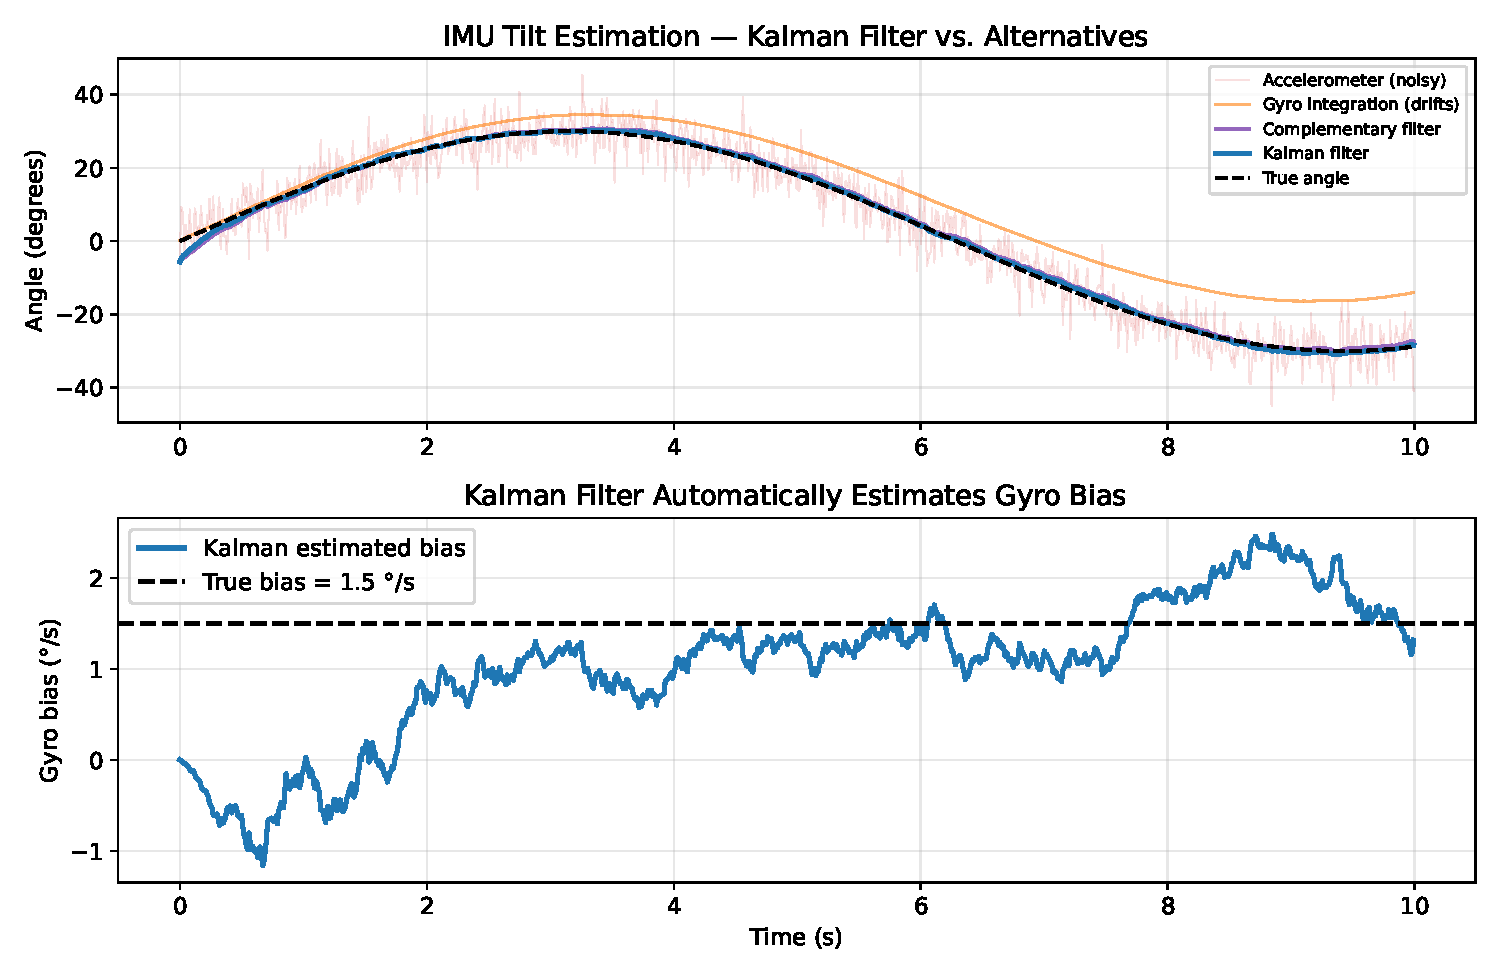
\includegraphics[width=\textwidth]{kalman_filter.pdf}
\caption{顶部：IMU 倾斜角估计对比。纯陀螺仪积分（橙色）严重漂移。加速度计（红色，浅）有噪声。互补滤波器（紫色）和卡尔曼滤波器（蓝色）都能跟踪真实角度（黑色虚线），但卡尔曼更平滑。底部：卡尔曼滤波器自动估计并收敛到 1.5\textdegree/s 的真实陀螺仪偏差。}
\end{figure}

\vspace{0.5em}
\begin{mdframed}[linewidth=1pt, innertopmargin=10pt, innerbottommargin=10pt]
\textbf{案例研究：LQR 平衡机器人——从方程到实际驾驭}

\vspace{0.3em}
给一个两轮自平衡机器人（类似 Segway）设计控制器。这是现代控制的"Hello World"，能很直观地展示为什么 MIMO 系统用 LQR + 卡尔曼比 PID 更顺手。

\textbf{系统：} 一个两轮平台，有一个高耸的机身，必须在保持直立的同时跟踪期望位置。

\textbf{状态：} $\mathbf{x} = \begin{bmatrix} \theta & \dot{\theta} & x & \dot{x} \end{bmatrix}^T$，其中 $\theta$ 是倾斜角，$x$ 是车轮位置。

\textbf{MIMO 的麻烦：}要往前走，机器人得先向\textit{前}倾（就像人要先弯腰才能迈步）。但倾斜恰恰是我们要避免的！位置控制和平衡\textbf{耦合且矛盾}。PID 至少要两个嵌套环路，还得小心处理耦合。LQR 一个增益矩阵 $K = [k_1, k_2, k_3, k_4]$ 全部搞定：
\[
u = -k_1 \theta - k_2 \dot{\theta} - k_3 (x - x_{\text{ref}}) - k_4 \dot{x}
\]

\textbf{通过 Q 和 R 调参：}
\begin{itemize}[nosep]
    \item 想要激进的平衡？增大 $Q_{11}$（惩罚倾斜角）。
    \item 想要精确的位置跟踪？增大 $Q_{33}$（惩罚位置误差）。
    \item 电机功率不足？增大 $R$（惩罚控制代价）。
\end{itemize}

一个典型的起始点：$Q = \text{diag}(100, 1, 10, 1)$，$R = 1$。意思是："倾斜角我比速度在乎 100 倍，位置比速度在乎 10 倍。"MATLAB 里跑一行 \texttt{K = lqr(A, B, Q, R)}，四个增益往下灌，机器人就能立起来了。

\textbf{完整系统：}
\begin{enumerate}[nosep]
    \item \textbf{卡尔曼滤波器} 从 IMU + 车轮编码器估计 $[\theta, \dot{\theta}, x, \dot{x}]$。
    \item \textbf{LQR 控制器} 从估计状态计算电机力矩。
    \item 两者均以 500--1000 Hz 在 STM32 上运行。
\end{enumerate}

卡尔曼 + LQR，这个组合就是平衡机器人、无人机姿态控制以及一切多状态耦合系统的标配。
\end{mdframed}

\begin{figure}[H]
\centering
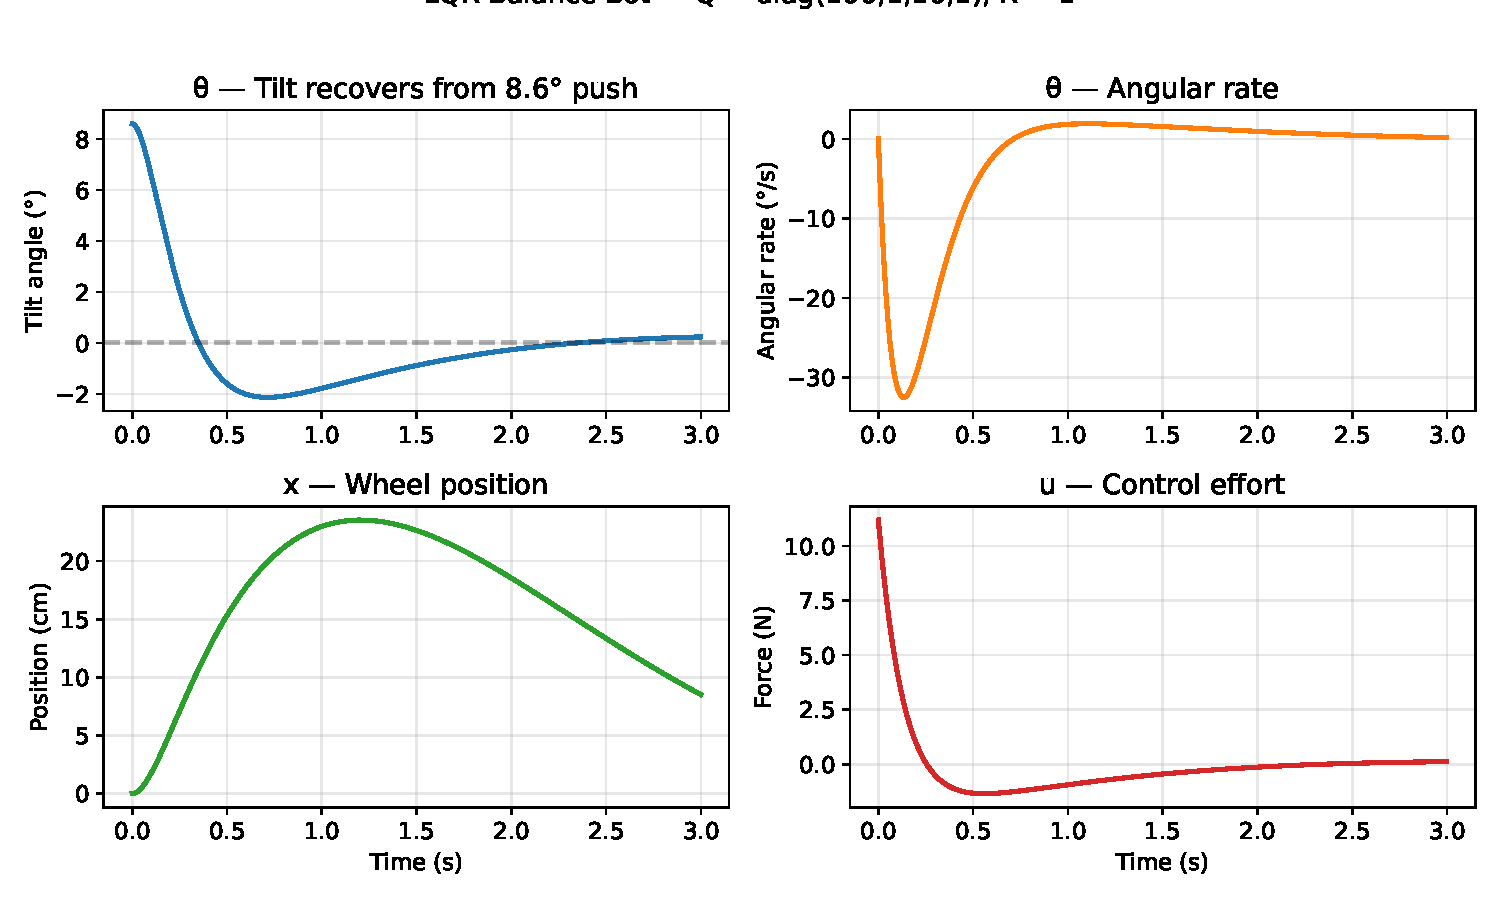
\includegraphics[width=\textwidth]{lqr_balance.pdf}
\caption{LQR 平衡机器人仿真。从 8.6\textdegree{} 的初始倾斜开始，控制器将四个状态全部恢复到零。左上：倾斜角在约 1 秒内收敛。右上：角速度。左下：车轮向后移动以承接下落的机身，然后归位。右下：控制力——注意初始的大幅脉冲，随后平稳衰减。}
\end{figure}

\newpage

\subsection{轨迹生成（Trajectory Generation）：告诉电机去哪里}

直接把指令从 $0°$ 跳到 $90°$，别指望有好结果——电机又不会瞬移。你需要一条平滑的\textbf{参考轨迹}，位置、速度、加速度都得规划好，而且要尊重执行器的物理极限。没有轨迹规划，PID 上来就饱和，积分往死里攒，等电机好不容易靠近 $90°$，控制器已经在跟自己打架了。轨迹生成，就是"我的炮塔能用"和"我的炮塔跟强队一个水平"之间的分水岭。

\subsubsection{梯形速度曲线（Trapezoidal Velocity Profile）}

梯形曲线是运动控制的主力。给定移动距离 $d$、最大速度 $v_{\max}$ 和最大加速度 $a_{\max}$，产生三个阶段：

\begin{enumerate}[nosep]
    \item 从静止以 $a_{\max}$ \textbf{加速}至 $v_{\max}$
    \item 以 $v_{\max}$ \textbf{匀速}行驶
    \item 以 $-a_{\max}$ \textbf{减速}回到静止
\end{enumerate}

\textbf{时间与距离：}
\begin{align}
t_{\text{加速}} &= \frac{v_{\max}}{a_{\max}}, \qquad
d_{\text{加速}} = \frac{1}{2}a_{\max}t_{\text{加速}}^2, \qquad
d_{\text{匀速}} = d - 2\,d_{\text{加速}}
\end{align}

如果 $d_{\text{匀速}} < 0$，距离不足以达到 $v_{\max}$。曲线变为\textbf{三角形}：电机加速至峰值速度 $v_{\text{peak}} = \sqrt{a_{\max}\,d}$ 后立即减速，没有匀速阶段。

\textbf{时刻 $t$ 的参考信号：}

令 $t_1 = t_{\text{加速}}$，$t_2 = t_1 + d_{\text{匀速}}/v_{\max}$，$t_3 = t_2 + t_{\text{加速}}$。

\begin{equation}
\theta_{\text{ref}}(t) = \begin{cases}
\tfrac{1}{2}a_{\max}t^2 & 0 \le t < t_1 \quad \text{（加速段）}\\[4pt]
d_{\text{加速}} + v_{\max}(t - t_1) & t_1 \le t < t_2 \quad \text{（匀速段）}\\[4pt]
d - \tfrac{1}{2}a_{\max}(t_3-t)^2 & t_2 \le t \le t_3 \quad \text{（减速段）}
\end{cases}
\end{equation}

\begin{equation}
\dot{\theta}_{\text{ref}}(t) = \begin{cases}
a_{\max}\,t & 0 \le t < t_1 \\
v_{\max} & t_1 \le t < t_2 \\
a_{\max}(t_3 - t) & t_2 \le t \le t_3
\end{cases}
\qquad
\ddot{\theta}_{\text{ref}}(t) = \begin{cases}
+a_{\max} & 0 \le t < t_1 \\
0 & t_1 \le t < t_2 \\
-a_{\max} & t_2 \le t \le t_3
\end{cases}
\end{equation}

这三个信号是实现完整前馈增强控制器所需的全部内容（更多内容见下面的实践框）。

\subsubsection{S形速度曲线（S-Curve Profile）}

梯形曲线的加速度是不连续的——瞬间从 $0$ 跳变到 $a_{\max}$。这种突然的冲击（jerk）会激励机械共振，磨损齿轮，引起振动。\textbf{S形曲线}（或限制冲击的曲线）增加了第七个约束：加速度的变化率（冲击，$j_{\max}$）受到限制。

这将三段式梯形曲线变为七段式曲线：
\begin{enumerate}[nosep]
    \item 冲击增加（加速度从0增加到 $a_{\max}$）
    \item 恒定加速度 $a_{\max}$
    \item 冲击减小（加速度从 $a_{\max}$ 减小到0）
    \item 以 $v_{\max}$ 匀速行驶
    \item 冲击减小（加速度变为 $-a_{\max}$）
    \item 恒定减速度 $-a_{\max}$
    \item 冲击增加（回到零加速度）
\end{enumerate}

结果是一个处处二阶连续可微的位置曲线——平滑到云台和精密机构几乎感觉不到运动开始。数学推导较为复杂，但实践中你很少需要从头实现：运动控制库（WPILib的 \texttt{TrapezoidProfile}、REV的Motion Magic等）已经帮你处理好了。

\begin{mdframed}[linewidth=1pt, innertopmargin=10pt, innerbottommargin=10pt]
\textbf{实践：如何选择曲线类型}

\vspace{0.3em}
\textbf{梯形曲线}适合90\%的竞赛应用：
\begin{itemize}[nosep]
    \item 驱动轮、飞轮、炮塔旋转
    \item 实现和调试简单——三段、分段公式
    \item 足够好用，除非你听到齿轮震颤或看到快速运动时的振荡
\end{itemize}

\textbf{S形曲线}适用于对平滑性要求严苛的场合：
\begin{itemize}[nosep]
    \item 云台和双轴稳定平台
    \item 精密定位机构（相机滑轨、基于编码器的机械臂）
    \item 任何担心齿轮磨损或振动的场合
\end{itemize}

\textbf{跟踪轨迹炮塔的完整前馈链：}

在每个控制时间步，轨迹规划器输出三个数：$\theta_{\text{ref}}$、$\dot{\theta}_{\text{ref}}$、$\ddot{\theta}_{\text{ref}}$。全部利用起来：
\[
u = \underbrace{K_p\bigl(\theta_{\text{ref}} - \theta\bigr) + K_i\int(\cdot)\,dt + K_d\dot{e}}_{\text{外位置PID}}
  + \underbrace{k_v\,\dot{\theta}_{\text{ref}}}_{\text{速度前馈}}
  + \underbrace{k_a\,\ddot{\theta}_{\text{ref}}}_{\text{加速度前馈}}
\]

加速度前馈来自旋转的牛顿第二定律：$\tau = J\alpha$，因此 $k_a \approx J / k_{\tau}$，其中 $k_\tau$ 是电机的力矩常数。位置PID只需消除小的跟踪误差；前馈承担主要工作。
\end{mdframed}

\begin{figure}[H]
\centering
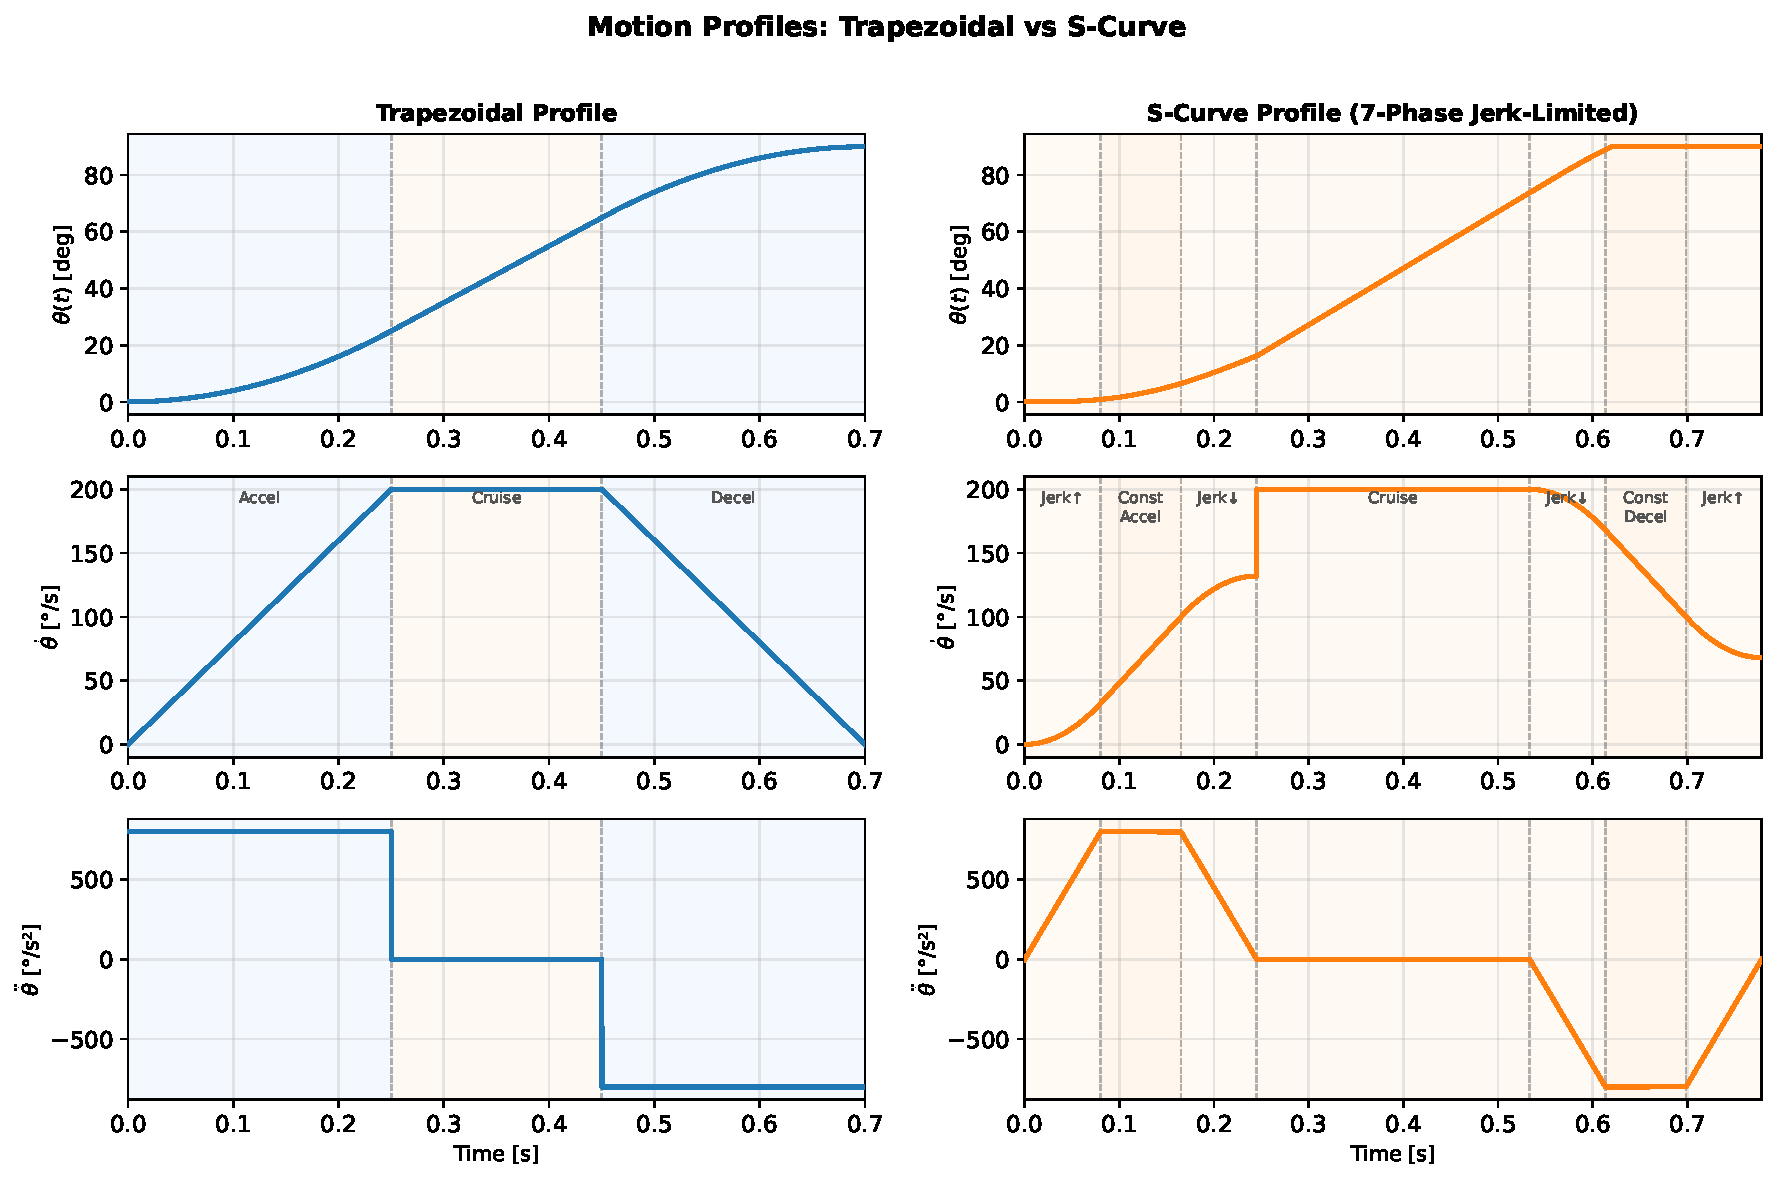
\includegraphics[width=\textwidth]{trajectory_profiles.pdf}
\caption{90°运动的梯形曲线（左）与S形曲线（右）对比。梯形曲线的加速度不连续（突然跳变），而S形曲线限制冲击以实现更平滑的运动。两者都生成用于前馈控制的位置、速度和加速度参考信号。}
\end{figure}

\subsubsection{B\'{e}zier 曲线与样条插值}

梯形曲线和S形曲线适用于单段点到点运动，但许多应用场景需要在二维或三维空间中沿多个路径点生成平滑轨迹。\textbf{B\'{e}zier 曲线}和\textbf{三次样条}是实现该目标的两种常用工具。

\paragraph{B\'{e}zier 曲线。}
$n$ 次 B\'{e}zier 曲线由 $n+1$ 个\textbf{控制点} $\mathbf{P}_0, \mathbf{P}_1, \ldots, \mathbf{P}_n$ 定义，其参数化形式为（$t \in [0,1]$）：
\[
\mathbf{B}(t) = \sum_{i=0}^{n} \binom{n}{i}(1-t)^{n-i}\,t^{i}\,\mathbf{P}_i
\]
最常用的是\textbf{三次 B\'{e}zier 曲线}（$n=3$），使用四个控制点。曲线经过 $\mathbf{P}_0$（$t=0$）和 $\mathbf{P}_3$（$t=1$），而 $\mathbf{P}_1$ 和 $\mathbf{P}_2$ 控制曲线形状但不在曲线上。其关键性质在于：曲线在 $\mathbf{P}_0$ 处的切线指向 $\mathbf{P}_1$，在 $\mathbf{P}_3$ 处的切线从 $\mathbf{P}_2$ 方向出发——这为进出方向提供了直观的控制手段。B\'{e}zier 曲线适用于需要平滑曲线且可控进出方向的\textbf{路径点规划}场景（如全向驱动路径、机械臂末端执行器轨迹等）。

\paragraph{三次样条插值。}
若需经过一组路径点 $\{q_0, q_1, \ldots, q_N\}$，可采用在路径点处拼接的\textbf{分段三次多项式}。每段的形式为：
\[
q_i(t) = a_i + b_i\,t + c_i\,t^2 + d_i\,t^3
\]
在各拼接点处，\textbf{连续性条件}要求相邻段的位置、速度和加速度相匹配，从而获得 $C^2$ 连续性（直到二阶导数连续）。常用的边界条件有两种：
\begin{itemize}
    \item \textbf{自然样条}：两端点处的二阶导数为零。
    \item \textbf{固定样条}：在两端点处指定速度（一阶导数）。
\end{itemize}
与 B\'{e}zier 曲线相比，三次样条\textbf{保证经过所有路径点}——B\'{e}zier 曲线仅经过首尾两个控制点。与梯形曲线相比，三次样条在全程提供\textbf{光滑的速度和加速度}，不存在不连续点。

\paragraph{适用场景对比。}
\begin{itemize}
    \item \textbf{梯形/S形曲线}：具有明确速度和加速度限制的单段点到点运动。
    \item \textbf{B\'{e}zier 曲线}：需要形状控制的平滑二维/三维路径（如全向驱动路径、末端执行器轨迹）。
    \item \textbf{三次样条}：需要经过每个路径点的多点轨迹（如自主导航序列）。
\end{itemize}

\begin{figure}[H]
\centering
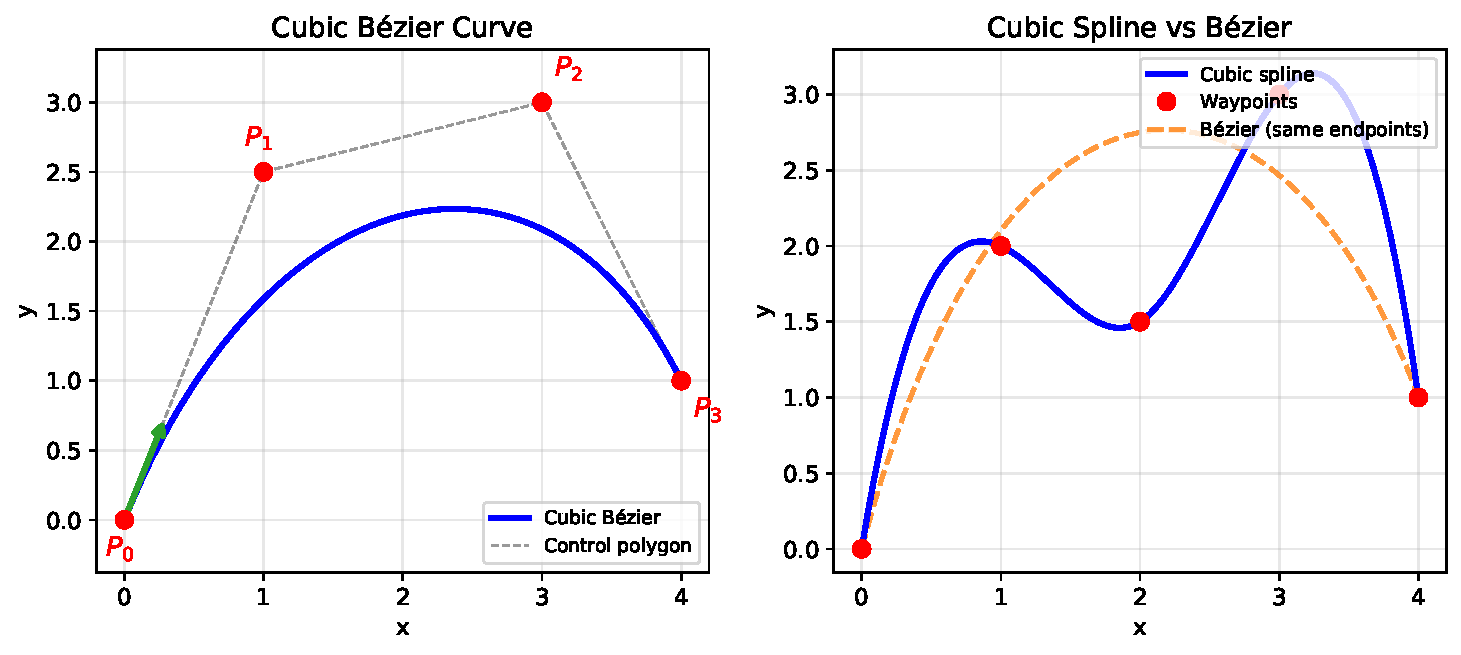
\includegraphics[width=\textwidth]{bezier_spline.pdf}
\caption{左图：三次 B\'{e}zier 曲线由四个控制点 $P_0$--$P_3$ 定义，曲线经过 $P_0$ 和 $P_3$，$P_1$ 和 $P_2$ 控制曲线形状。绿色和红色箭头表示端点处的切线方向。右图：三次样条插值保证经过所有路径点（红点），而 B\'{e}zier 曲线仅经过首尾两个控制点。}
\end{figure}

\newpage

%=============================================================================
\section{Attitude and Rotation Representation}
%=============================================================================

Before we can estimate or control orientation (Ch6 uses Euler angles and quaternions extensively), we need a solid foundation in how rotations work mathematically. This chapter builds that foundation from scratch.

Why does this matter for robotics? Every time you read an IMU, command a gimbal, or fuse sensor data in an EKF, you are working with rotations. Get the math wrong---mix up a convention, compose rotations in the wrong order, or hit a singularity---and your robot will do something unexpected. The good news: the core ideas are not hard. They just need to be understood once, carefully.

%-----------------------------------------------------------------------------
\subsection{Coordinate Frames}
%-----------------------------------------------------------------------------

All of 3D robotics begins with a choice: \textit{which way do the axes point?}

\subsubsection{The Right-Hand Rule}

Hold out your right hand. Point your thumb along the $x$-axis, your index finger along $y$, and curl your middle finger---it points along $z$. This is a \textbf{right-handed coordinate frame}, and it is the universal standard in robotics and aerospace.

Several conventions exist that all use the right-hand rule but differ in axis assignment. In this book, we adopt:

\textbf{NWU (North-West-Up):} $x$ points north (forward), $y$ points west (left), $z$ points up. This is the convention used throughout our competition robots---forward is $+x$, left is $+y$, up is $+z$. It is a right-handed frame and matches the body-frame convention where $x$ is ``forward.''

Other common conventions you will encounter:
\begin{itemize}[nosep]
    \item \textbf{NED (North-East-Down):} $x$ north, $y$ east, $z$ down. Standard in aerospace and many IMU datasheets. Positive $z$ is ``down,'' so altitude is negative $z$.
    \item \textbf{ENU (East-North-Up):} $x$ east, $y$ north, $z$ up. Common in ROS and geographic mapping.
\end{itemize}

All three are perfectly valid right-handed frames. The critical thing is to pick one and be consistent. If your IMU outputs NED data and your control algorithm expects NWU, you need to convert ($y_{\text{NWU}} = -y_{\text{NED}}$, $z_{\text{NWU}} = -z_{\text{NED}}$). This is one of the most common sources of bugs in robotics software.

\begin{figure}[H]
  \centering
  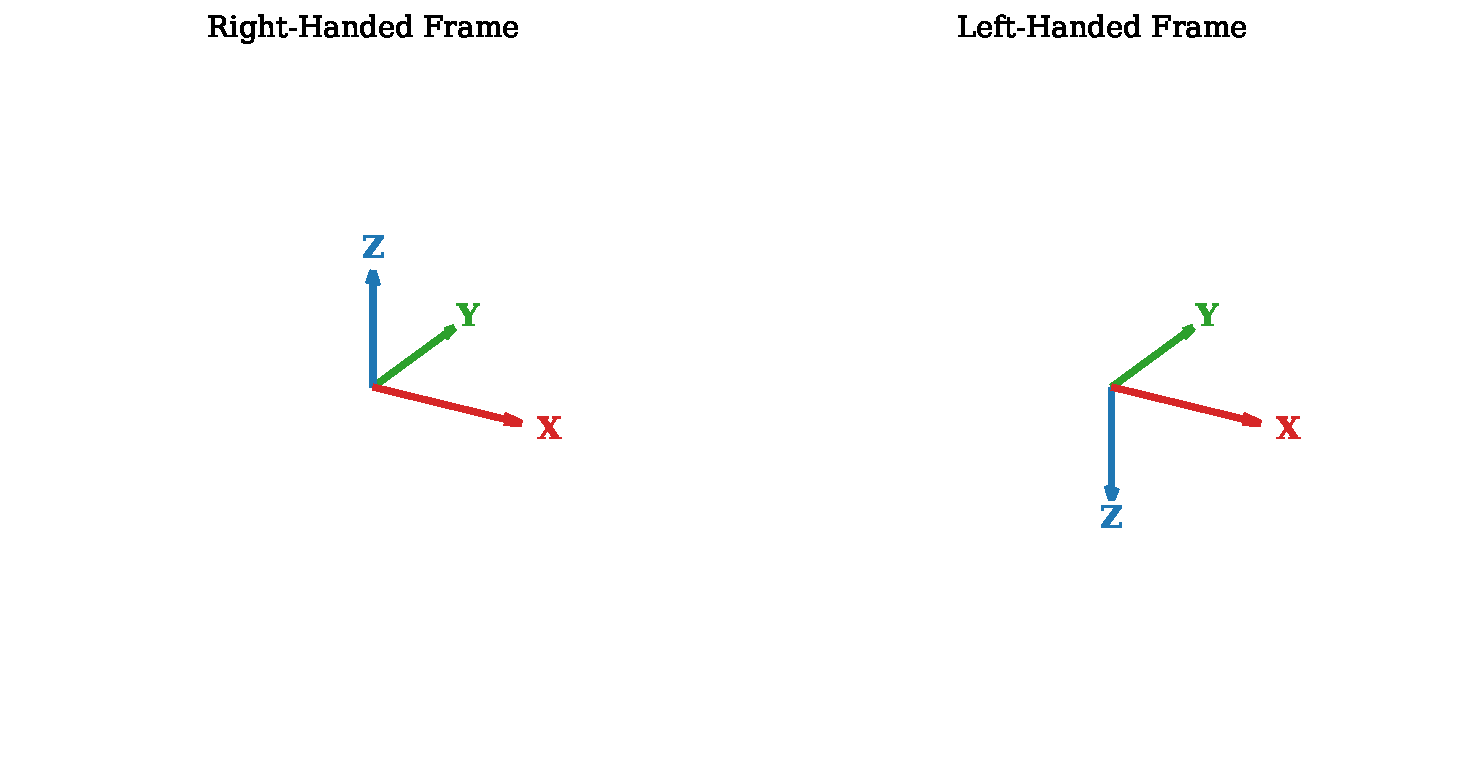
\includegraphics[width=\textwidth]{coord_rh_lh.pdf}
  \caption{Right-handed vs left-handed coordinate frames. In a right-handed frame, the cross product $\hat{x} \times \hat{y} = \hat{z}$; in a left-handed frame, $\hat{x} \times \hat{y} = -\hat{z}$.}
\end{figure}

\subsubsection{Right-Hand vs Left-Hand Frames}

A \textbf{left-handed} frame is what you get if you use your left hand instead. Some graphics engines (notably DirectX and Unity's default) use left-handed frames because it makes the $z$-axis point ``into the screen,'' which is convenient for rendering. Most robotics software uses right-handed frames. If you mix conventions---say, importing a mesh from a left-handed graphics tool into a right-handed robotics simulator---rotations will appear mirrored. Always check the convention.

\subsubsection{Common Frames in Robotics}

Two frames appear in virtually every robotics problem:

\begin{itemize}[nosep]
    \item \textbf{World (inertial) frame:} Fixed to the ground (or to the Earth, if you are working at scales where Earth's rotation matters). This is the ``global'' reference. We often denote it with a superscript $W$ or subscript $\text{world}$.
    \item \textbf{Body frame:} Fixed to the robot. It moves and rotates with the robot. In our NWU convention, $x$ points forward, $y$ points left, and $z$ points up. Denoted with $B$ or $\text{body}$.
\end{itemize}

The central question of attitude representation is: \textit{how do we describe the orientation of the body frame relative to the world frame?}

\begin{figure}[H]
  \centering
  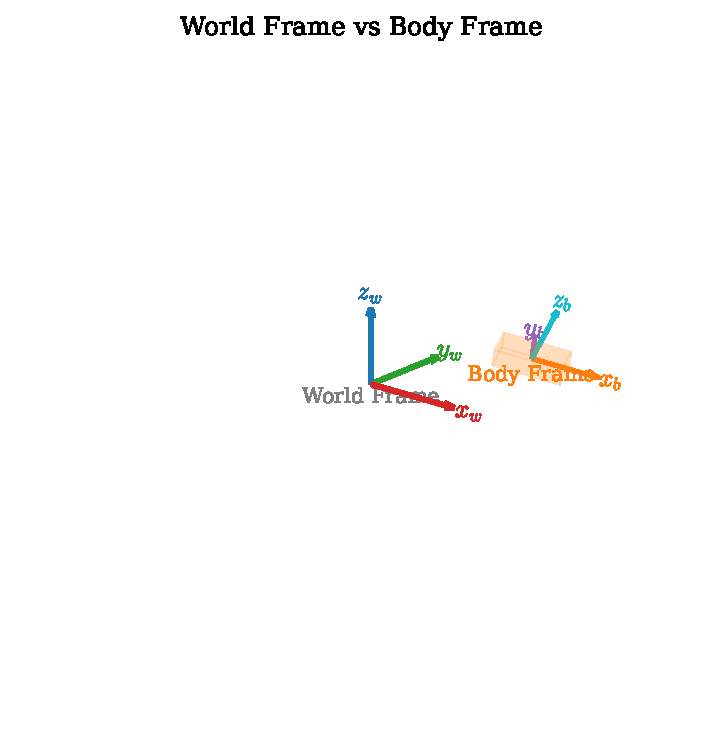
\includegraphics[width=0.75\textwidth]{coord_world_body.pdf}
  \caption{World frame (fixed) and body frame (moves with the robot). The rotation matrix $R$ describes how the body frame is oriented relative to the world frame.}
\end{figure}

%-----------------------------------------------------------------------------
\subsection{Rotation Matrices}
%-----------------------------------------------------------------------------

\subsubsection{Definition and Properties}

A rotation matrix $R$ is a $3 \times 3$ matrix that belongs to the \textbf{special orthogonal group} $\mathrm{SO}(3)$:
\begin{equation}
\mathrm{SO}(3) = \{ R \in \mathbb{R}^{3 \times 3} \mid R^T R = I, \; \det(R) = +1 \}
\end{equation}

The condition $R^T R = I$ (orthogonality) means the columns of $R$ are mutually perpendicular unit vectors. The condition $\det(R) = +1$ distinguishes proper rotations from reflections (which have $\det = -1$).

\textbf{Physical meaning:} Each column of $R$ tells you where the corresponding original basis vector ends up after the rotation. If $R = [\mathbf{r}_1 \; \mathbf{r}_2 \; \mathbf{r}_3]$, then $\mathbf{r}_1$ is the image of $\hat{x}$, $\mathbf{r}_2$ is the image of $\hat{y}$, and $\mathbf{r}_3$ is the image of $\hat{z}$. Equivalently, the \textit{rows} of $R$ are the body-frame axes expressed in world coordinates.

The three elementary rotation matrices (counterclockwise when looking from the positive axis toward the origin) are:

\begin{equation}
R_x(\theta) = \begin{bmatrix} 1 & 0 & 0 \\ 0 & \cos\theta & -\sin\theta \\ 0 & \sin\theta & \cos\theta \end{bmatrix}
\end{equation}

\begin{equation}
R_y(\theta) = \begin{bmatrix} \cos\theta & 0 & \sin\theta \\ 0 & 1 & 0 \\ -\sin\theta & 0 & \cos\theta \end{bmatrix}
\end{equation}

\begin{equation}
R_z(\theta) = \begin{bmatrix} \cos\theta & -\sin\theta & 0 \\ \sin\theta & \cos\theta & 0 \\ 0 & 0 & 1 \end{bmatrix}
\end{equation}

Note the ``odd one out'': $R_y$ has the $-\sin\theta$ in the top-right and $+\sin\theta$ in the bottom-left, which is the transpose of what you might expect. This is because the $y$-axis rotation cycles $z \to x$ (not $x \to z$), and consistency with the right-hand rule requires the sign flip.

\subsubsection{What Rotation Matrices Actually Do}

There are two ways to interpret the same rotation matrix, and confusing them is a guaranteed source of bugs.

\textbf{Interpretation 1: Active (alibi) rotation.} The matrix physically rotates a vector to a new position in the \textit{same} coordinate frame. Think of grabbing a vector and spinning it.

\textbf{Interpretation 2: Passive (alias) rotation.} The matrix re-expresses the same physical vector in a \textit{different} coordinate frame. The vector does not move; we just describe it from a new viewpoint.

Mathematically, the active rotation of $\mathbf{v}$ by angle $\theta$ about the $z$-axis and the passive transformation from frame $A$ to frame $B$ (where $B$ is rotated by $-\theta$ relative to $A$) use the same matrix. The difference is purely in interpretation.

For robotics, the most important convention is:
\begin{equation}
\mathbf{v}_{\text{world}} = R \, \mathbf{v}_{\text{body}}
\quad \Longleftrightarrow \quad
\mathbf{v}_{\text{body}} = R^T \mathbf{v}_{\text{world}}
\end{equation}

Here $R$ is the rotation matrix that transforms vectors from the body frame to the world frame (sometimes written $R^W_B$ or $R_{\text{body} \to \text{world}}$). To go the other way, use $R^T = R^{-1}$---the beauty of orthogonal matrices is that the inverse is just the transpose.

\begin{figure}[H]
  \centering
  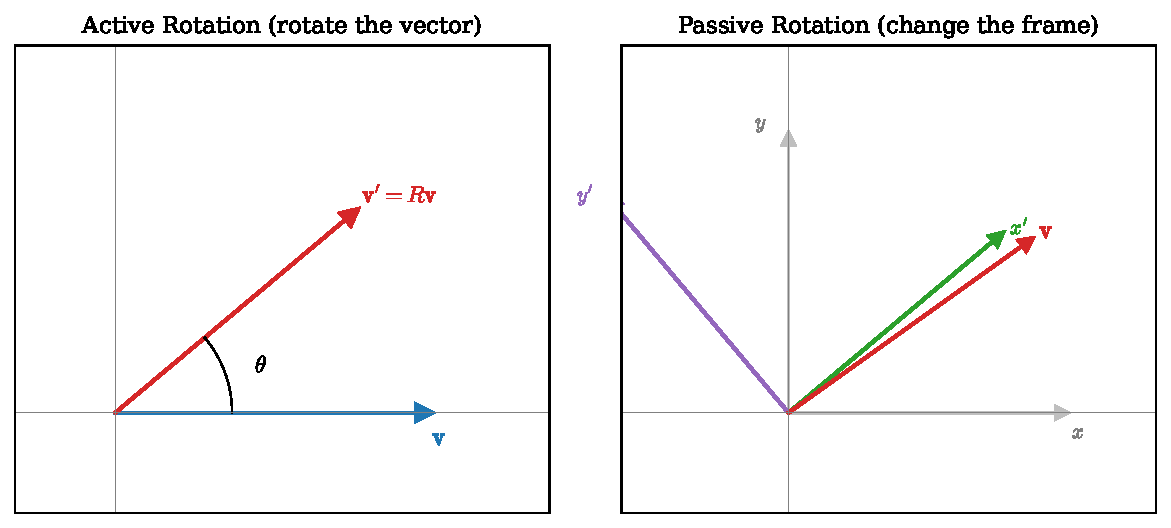
\includegraphics[width=0.85\textwidth]{rotation_active_passive.pdf}
  \caption{Two interpretations of the same rotation matrix. Active: the vector moves. Passive: the coordinate frame moves. Both use the same $R$, but the conceptual picture is different.}
\end{figure}

\vspace{0.5em}
\begin{mdframed}[linewidth=1pt, innertopmargin=10pt, innerbottommargin=10pt]
\textbf{The \#1 source of confusion:} Different textbooks and libraries use opposite conventions. Some define $R$ as world-to-body; others as body-to-world. When you import a rotation matrix from a library, \textit{always check which convention it uses}. If you get it backwards, every transformed vector will be wrong, and the error will look like your robot is mirrored or spinning the wrong way.
\end{mdframed}

\subsubsection{Composing Rotations: Left vs Right Multiplication}

Suppose you want to apply rotation $R_1$ first, then rotation $R_2$. The combined rotation is:
\begin{equation}
R_{\text{total}} = R_2 \cdot R_1
\end{equation}

This is \textbf{right-to-left} order: the rotation applied first is on the right. This follows from the associativity of matrix multiplication: $R_2 (R_1 \mathbf{v}) = (R_2 R_1) \mathbf{v}$.

Now, here is where things get subtle. There are two ways to build up a sequence of rotations:

\textbf{Extrinsic rotations (world-fixed axes):} Each successive rotation is about an axis of the fixed world frame. The total rotation is built by \textit{pre-multiplying} (multiplying on the left):
\[
R_{\text{total}} = R_3 \cdot R_2 \cdot R_1
\]
Read left-to-right: $R_3$ is the last rotation applied, but it acts about a world-fixed axis.

\textbf{Intrinsic rotations (body-fixed axes):} Each successive rotation is about an axis of the current (already-rotated) body frame. The total rotation is built by \textit{post-multiplying} (multiplying on the right):
\[
R_{\text{total}} = R_1 \cdot R_2 \cdot R_3
\]
Here $R_1$ rotates about the original body axis, $R_2$ about the once-rotated body axis, and so on.

A remarkable fact: an intrinsic $ZYX$ rotation (yaw about body $z$, then pitch about the new body $y$, then roll about the newest body $x$) produces the \textit{same} matrix as an extrinsic $XYZ$ rotation (roll about world $x$, then pitch about world $y$, then yaw about world $z$). The order reverses. This is purely a consequence of the associativity of matrix multiplication.

For the standard aerospace convention (intrinsic $ZYX$: yaw $\psi$, pitch $\theta$, roll $\phi$):
\begin{equation}
R = R_z(\psi) \cdot R_y(\theta) \cdot R_x(\phi)
\end{equation}

\textbf{Common pitfall:} Getting the multiplication order wrong compiles fine and runs fine---it just gives a subtly wrong orientation. There is no runtime error to alert you. Always write down the convention explicitly in your code comments.

%-----------------------------------------------------------------------------
\subsection{Euler Angles}
%-----------------------------------------------------------------------------

\begin{figure}[H]
  \centering
  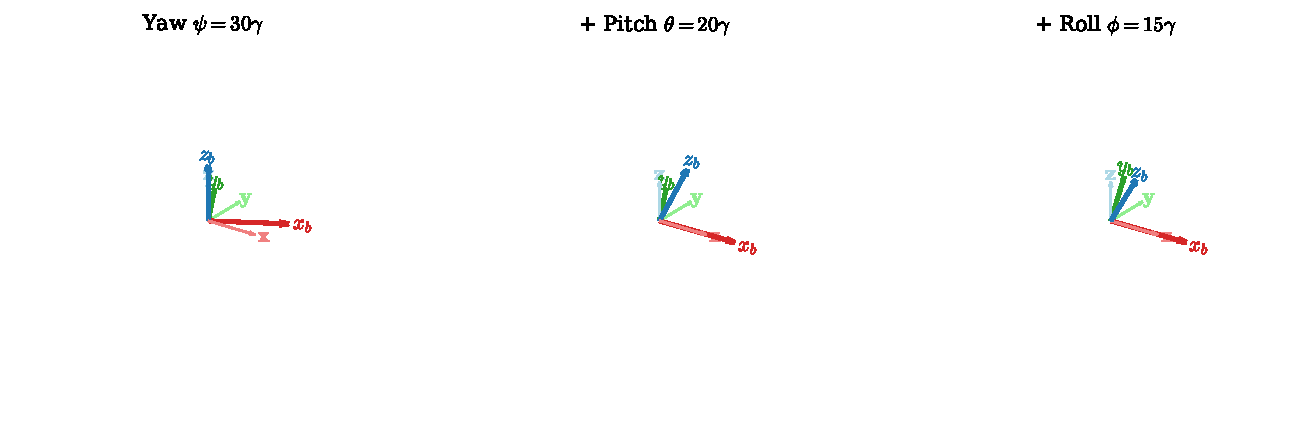
\includegraphics[width=\textwidth]{euler_angles.pdf}
  \caption{Building up a ZYX rotation step by step. Left: yaw only ($\psi = 30°$). Center: yaw + pitch ($\theta = 20°$). Right: yaw + pitch + roll ($\phi = 15°$). Faint axes show the world frame; bold axes show the body frame.}
\end{figure}

\subsubsection{Definition and Conventions}

Euler angles describe an arbitrary rotation as a sequence of three elementary rotations about coordinate axes. There are 12 possible sequences (6 ``proper'' Euler angles like $ZXZ$, $ZYZ$, etc., and 6 Tait--Bryan angles like $ZYX$, $XYZ$, etc.). The most common in robotics and aerospace is the \textbf{ZYX} (yaw-pitch-roll) convention:

\begin{enumerate}[nosep]
    \item Yaw ($\psi$): rotate about the $z$-axis.
    \item Pitch ($\theta$): rotate about the (new) $y$-axis.
    \item Roll ($\phi$): rotate about the (newest) $x$-axis.
\end{enumerate}

The resulting rotation matrix is (intrinsic $ZYX$):
\begin{equation}
R = R_z(\psi) \, R_y(\theta) \, R_x(\phi)
\end{equation}

Expanding this product fully using the elementary matrices:

\begin{equation}
R = \begin{bmatrix}
c_\psi c_\theta & c_\psi s_\theta s_\phi - s_\psi c_\phi & c_\psi s_\theta c_\phi + s_\psi s_\phi \\
s_\psi c_\theta & s_\psi s_\theta s_\phi + c_\psi c_\phi & s_\psi s_\theta c_\phi - c_\psi s_\phi \\
-s_\theta & c_\theta s_\phi & c_\theta c_\phi
\end{bmatrix}
\end{equation}

where $c_\psi = \cos\psi$, $s_\psi = \sin\psi$, etc.

\textbf{Extracting Euler angles from a rotation matrix.} Given a rotation matrix $R = [r_{ij}]$, the ZYX Euler angles can be recovered as:
\begin{align}
\theta &= -\arcsin(r_{31}) \\
\phi &= \operatorname{atan2}(r_{32}, \, r_{33}) \\
\psi &= \operatorname{atan2}(r_{21}, \, r_{11})
\end{align}

The use of $\operatorname{atan2}$ (which takes two arguments and returns the angle in the correct quadrant) is essential. Using $\arctan$ alone would give ambiguous results.

\subsubsection{Gimbal Lock}

Gimbal lock is the Achilles' heel of Euler angles, and it is the single most important reason to learn quaternions.

\textbf{What is it?} When the pitch angle reaches $\theta = \pm 90°$, the yaw and roll axes become aligned---they rotate about the same physical axis. The system loses one degree of freedom. You can still represent the current orientation, but you cannot distinguish certain rotations near the singularity, and small changes in orientation cause wild jumps in the Euler angles.

\textbf{Mathematical demonstration.} Set $\theta = 90°$ (so $\cos\theta = 0$ and $\sin\theta = 1$) in the rotation matrix:

\begin{equation}
R\big|_{\theta=90°} = \begin{bmatrix}
0 & \cos\psi \sin\phi - \sin\psi \cos\phi & \cos\psi \cos\phi + \sin\psi \sin\phi \\
0 & \sin\psi \sin\phi + \cos\psi \cos\phi & \sin\psi \cos\phi - \cos\psi \sin\phi \\
-1 & 0 & 0
\end{bmatrix}
\end{equation}

Using the angle subtraction identities, this simplifies to:
\begin{equation}
R\big|_{\theta=90°} = \begin{bmatrix}
0 & -\sin(\psi - \phi) & \cos(\psi - \phi) \\
0 & \cos(\psi - \phi) & \sin(\psi - \phi) \\
-1 & 0 & 0
\end{bmatrix}
\end{equation}

Notice: only the \textit{difference} $\psi - \phi$ appears. We have three parameters ($\psi, \theta, \phi$) but only two are independent at this configuration---one degree of freedom is lost. There are infinitely many $(\psi, \phi)$ pairs that give the same rotation, as long as their difference is the same.

\textbf{Physical analogy.} Imagine a three-axis gimbal (like on a camera stabilizer). The inner ring controls roll, the middle ring controls pitch, and the outer ring controls yaw. When the middle ring tilts to $90°$, the inner and outer rings become coplanar. Rotating the inner ring now produces the same motion as rotating the outer ring---you have lost the ability to independently control one axis.

\textbf{Why this matters in practice.} If you are running an EKF that tracks Euler angles as its state vector, the covariance matrix becomes singular near $\theta = \pm 90°$---the filter diverges. Even before reaching exactly $90°$, the kinematic equations that relate angular velocity $\boldsymbol{\omega}$ to Euler angle rates contain $\cos\theta$ in the denominator:
\begin{equation}
\begin{bmatrix} \dot{\phi} \\ \dot{\theta} \\ \dot{\psi} \end{bmatrix}
= \begin{bmatrix}
1 & \sin\phi \tan\theta & \cos\phi \tan\theta \\
0 & \cos\phi & -\sin\phi \\
0 & \sin\phi / \cos\theta & \cos\phi / \cos\theta
\end{bmatrix}
\boldsymbol{\omega}
\end{equation}

The $\tan\theta$ terms blow up as $\theta \to \pm 90°$. This is not a numerical precision issue---it is a fundamental topological limitation of representing $\mathrm{SO}(3)$ with only three parameters.

\begin{figure}[H]
  \centering
  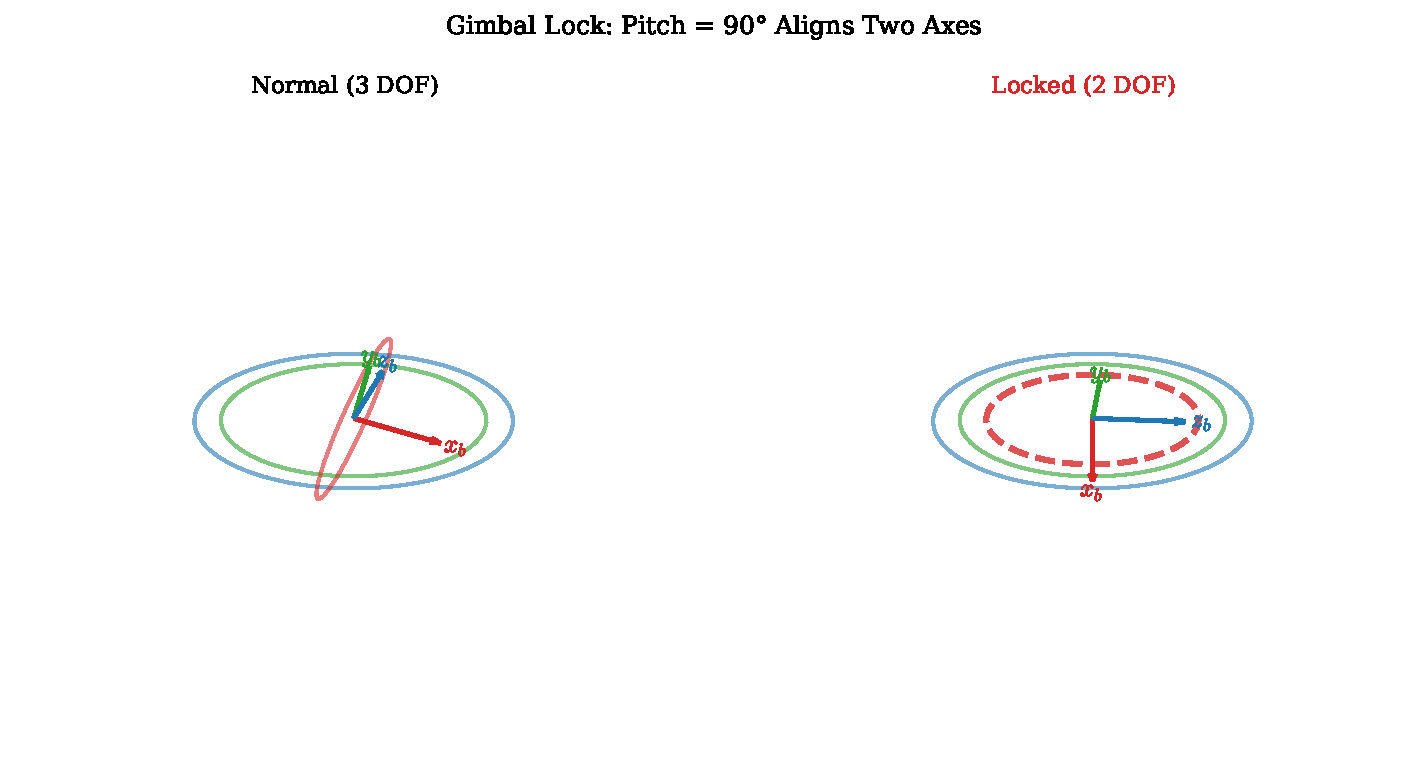
\includegraphics[width=0.85\textwidth]{gimbal_lock.pdf}
  \caption{Gimbal lock. Left: normal operation---the three gimbal rings provide three independent degrees of freedom. Right: when pitch reaches $90°$, the inner and outer rings align, collapsing yaw and roll into the same axis (dashed ring). One DOF is lost.}
\end{figure}

This motivates the search for a singularity-free representation: quaternions.

%-----------------------------------------------------------------------------
\subsection{Quaternions}
%-----------------------------------------------------------------------------

\subsubsection{Axis-Angle Rotation: The Gateway to Quaternions}

\begin{figure}[H]
  \centering
  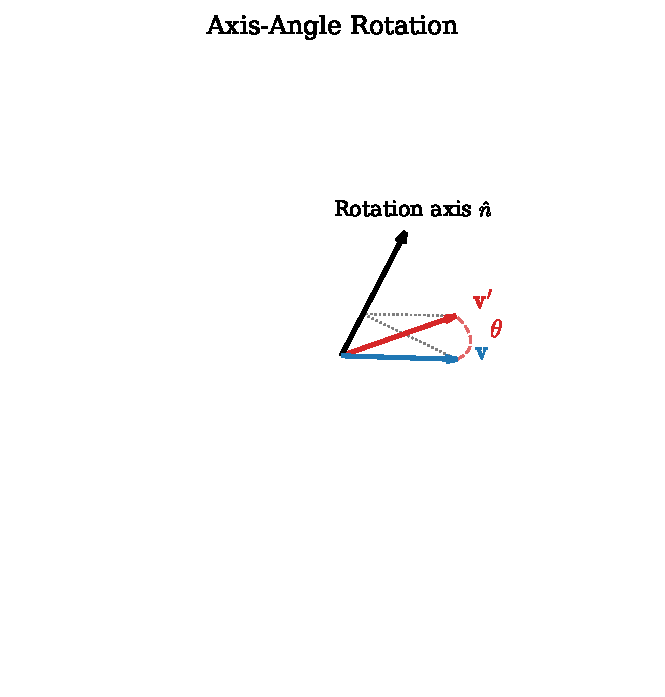
\includegraphics[width=0.6\textwidth]{axis_angle.pdf}
  \caption{Axis-angle rotation: vector $\mathbf{v}$ is rotated by angle $\theta$ about axis $\hat{n}$ to produce $\mathbf{v}'$. The dashed lines show the projection onto the rotation axis.}
\end{figure}

Before jumping to quaternions, we need one more concept. \textbf{Euler's rotation theorem} states that any rotation of a rigid body in 3D can be described by a single axis $\hat{n}$ (a unit vector) and a single angle $\theta$. No matter how complicated the rotation, there is always one axis that stays fixed, and the body has simply rotated around it.

This leads to \textbf{Rodrigues' rotation formula}, which rotates a vector $\mathbf{v}$ by angle $\theta$ about axis $\hat{n}$:
\begin{equation}
\mathbf{v}' = \mathbf{v} \cos\theta + (\hat{n} \times \mathbf{v}) \sin\theta + \hat{n} (\hat{n} \cdot \mathbf{v})(1 - \cos\theta)
\end{equation}

\textbf{Derivation.} Decompose $\mathbf{v}$ into a component parallel to $\hat{n}$ and a component perpendicular to $\hat{n}$:
\[
\mathbf{v}_\parallel = \hat{n}(\hat{n} \cdot \mathbf{v}), \qquad \mathbf{v}_\perp = \mathbf{v} - \mathbf{v}_\parallel
\]
The parallel component is unchanged by rotation about $\hat{n}$: $\mathbf{v}'_\parallel = \mathbf{v}_\parallel$. The perpendicular component rotates in the plane spanned by $\mathbf{v}_\perp$ and $\hat{n} \times \mathbf{v}$ (which is perpendicular to both $\hat{n}$ and $\mathbf{v}_\perp$, and has the same magnitude as $\mathbf{v}_\perp$):
\[
\mathbf{v}'_\perp = \mathbf{v}_\perp \cos\theta + (\hat{n} \times \mathbf{v}) \sin\theta
\]
Adding the two components: $\mathbf{v}' = \mathbf{v}_\parallel + \mathbf{v}'_\perp = \hat{n}(\hat{n} \cdot \mathbf{v}) + (\mathbf{v} - \hat{n}(\hat{n} \cdot \mathbf{v}))\cos\theta + (\hat{n} \times \mathbf{v})\sin\theta$. Rearranging gives the formula above.

The corresponding rotation matrix form is:
\begin{equation}
R = I \cos\theta + (1 - \cos\theta) \hat{n}\hat{n}^T + \sin\theta \, [\hat{n}]_\times
\end{equation}

where $[\hat{n}]_\times$ is the \textbf{skew-symmetric matrix} of $\hat{n} = (n_1, n_2, n_3)$:
\begin{equation}
[\hat{n}]_\times = \begin{bmatrix} 0 & -n_3 & n_2 \\ n_3 & 0 & -n_1 \\ -n_2 & n_1 & 0 \end{bmatrix}
\end{equation}

This matrix has the property that $[\hat{n}]_\times \mathbf{v} = \hat{n} \times \mathbf{v}$ for any vector $\mathbf{v}$.

\subsubsection{From Axis-Angle to Quaternions}

The axis-angle representation is intuitive, but it does not compose nicely: combining two axis-angle rotations requires going through rotation matrices or trigonometric identities. Quaternions solve this problem.

A \textbf{unit quaternion} encodes the same axis-angle rotation $(\hat{n}, \theta)$ as a four-component object:
\begin{equation}
q = \begin{bmatrix} \cos(\theta/2) \\ \sin(\theta/2) \, \hat{n} \end{bmatrix}
= \begin{bmatrix} q_w \\ q_x \\ q_y \\ q_z \end{bmatrix}
\end{equation}

where $q_w$ is the scalar (real) part and $(q_x, q_y, q_z)$ is the vector (imaginary) part.

\textbf{Why $\theta/2$ and not $\theta$?} This is the key insight. Quaternions live in a space where the algebraic structure (the Hamilton product, defined below) naturally composes rotations---but this only works with the half-angle encoding. The deep reason is topological: $\mathrm{SO}(3)$ is not simply connected, and the unit quaternion sphere $S^3$ is its \textbf{double cover}. This means that $q$ and $-q$ represent the \textit{same} rotation (negating all four components gives the same axis-angle pair with $\theta$ shifted by $2\pi$). This double-cover property is the price we pay for a singularity-free representation.

The set of unit quaternions satisfies $|q| = \sqrt{q_w^2 + q_x^2 + q_y^2 + q_z^2} = 1$, forming the 3-sphere $S^3$ in four-dimensional space.

\subsubsection{Quaternion Operations}

\textbf{Hamilton product (quaternion multiplication).} Given two quaternions $p = (p_w, \mathbf{p}_v)$ and $q = (q_w, \mathbf{q}_v)$ where $\mathbf{p}_v$ and $\mathbf{q}_v$ are the vector parts:
\begin{equation}
p \otimes q = \begin{bmatrix}
p_w q_w - \mathbf{p}_v \cdot \mathbf{q}_v \\
p_w \mathbf{q}_v + q_w \mathbf{p}_v + \mathbf{p}_v \times \mathbf{q}_v
\end{bmatrix}
\end{equation}

Written out component-wise:
\begin{equation}
p \otimes q = \begin{bmatrix}
p_w q_w - p_x q_x - p_y q_y - p_z q_z \\
p_w q_x + p_x q_w + p_y q_z - p_z q_y \\
p_w q_y - p_x q_z + p_y q_w + p_z q_x \\
p_w q_z + p_x q_y - p_y q_x + p_z q_w
\end{bmatrix}
\end{equation}

This product is \textbf{associative} $(p \otimes (q \otimes r) = (p \otimes q) \otimes r)$ but \textbf{not commutative} ($p \otimes q \neq q \otimes p$ in general). The non-commutativity reflects the physical fact that rotations in 3D do not commute.

\textbf{Rotating a vector.} To rotate a vector $\mathbf{v} \in \mathbb{R}^3$ by the rotation encoded in quaternion $q$, embed the vector as a ``pure quaternion'' $\bar{v} = (0, \mathbf{v})$ and compute:
\begin{equation}
\bar{v}' = q \otimes \bar{v} \otimes q^*
\end{equation}

where $q^*$ is the conjugate. The result $\bar{v}'$ is again a pure quaternion whose vector part is the rotated vector $\mathbf{v}'$. Why the double product? A single multiplication $q \otimes \bar{v}$ would not, in general, produce a pure quaternion (it could have a nonzero scalar part). The ``sandwich'' product $q \otimes \bar{v} \otimes q^*$ guarantees the scalar part vanishes, giving a proper 3D vector.

\textbf{Composing rotations.} Just like rotation matrices, quaternion rotations compose by multiplication, in the same right-to-left order:
\begin{equation}
q_{\text{total}} = q_2 \otimes q_1
\end{equation}

This means: ``first apply $q_1$, then apply $q_2$.'' To verify: $q_{\text{total}} \otimes \bar{v} \otimes q_{\text{total}}^* = q_2 \otimes (q_1 \otimes \bar{v} \otimes q_1^*) \otimes q_2^*$, which is indeed $q_1$ first, then $q_2$.

\textbf{Inverse and conjugate.} For a unit quaternion $q = (q_w, q_x, q_y, q_z)$:
\begin{equation}
q^{-1} = q^* = (q_w, -q_x, -q_y, -q_z)
\end{equation}

For unit quaternions, the inverse equals the conjugate (just like $R^{-1} = R^T$ for rotation matrices). This represents the reverse rotation.

\textbf{Quaternion to rotation matrix.} The rotation matrix corresponding to unit quaternion $q = (q_w, q_x, q_y, q_z)$ is:
\begin{equation}
R = \begin{bmatrix}
1 - 2(q_y^2 + q_z^2) & 2(q_x q_y - q_z q_w) & 2(q_x q_z + q_y q_w) \\
2(q_x q_y + q_z q_w) & 1 - 2(q_x^2 + q_z^2) & 2(q_y q_z - q_x q_w) \\
2(q_x q_z - q_y q_w) & 2(q_y q_z + q_x q_w) & 1 - 2(q_x^2 + q_y^2)
\end{bmatrix}
\end{equation}

You can verify that $R^T R = I$ and $\det(R) = 1$ using $q_w^2 + q_x^2 + q_y^2 + q_z^2 = 1$.

\textbf{Quaternion to Euler angles (ZYX convention).} Given $q = (q_w, q_x, q_y, q_z)$:
\begin{align}
\phi &= \operatorname{atan2}\!\big(2(q_w q_x + q_y q_z), \; 1 - 2(q_x^2 + q_y^2)\big) \\
\theta &= -\arcsin\!\big(2(q_x q_z - q_w q_y)\big) \\
\psi &= \operatorname{atan2}\!\big(2(q_w q_z + q_x q_y), \; 1 - 2(q_y^2 + q_z^2)\big)
\end{align}

These formulas follow directly from comparing the quaternion-to-matrix formula with the Euler angle matrix and applying the same extraction procedure.

\subsubsection{Why Quaternions Win}

Having seen both Euler angles and rotation matrices, here is why quaternions are the preferred representation for state estimation and control:

\textbf{No gimbal lock.} Quaternions parameterize $\mathrm{SO}(3)$ smoothly everywhere. There is no configuration where a degree of freedom is lost. The kinematic equation for quaternion propagation is:
\begin{equation}
\dot{q} = \frac{1}{2} q \otimes \begin{bmatrix} 0 \\ \boldsymbol{\omega} \end{bmatrix}
\end{equation}

where $\boldsymbol{\omega}$ is the angular velocity in the body frame. No tangent terms, no divisions by cosine, no singularities.

\textbf{Compact representation.} A quaternion uses 4 numbers, compared to 9 for a rotation matrix. It has only 1 constraint (unit norm) versus 6 constraints (orthogonality + unit determinant) for a rotation matrix. This makes quaternions easier to normalize and numerically more robust.

\textbf{Efficient composition.} The Hamilton product requires 16 multiplications and 12 additions. A $3 \times 3$ matrix product requires 27 multiplications and 18 additions. On a microcontroller, this difference adds up.

\textbf{Smooth interpolation.} Spherical Linear Interpolation (SLERP) provides the shortest, constant-speed path between two orientations on the quaternion sphere:
\begin{equation}
\text{SLERP}(q_0, q_1, t) = q_0 \frac{\sin((1-t)\Omega)}{\sin\Omega} + q_1 \frac{\sin(t\Omega)}{\sin\Omega}
\end{equation}

where $\Omega = \arccos(q_0 \cdot q_1)$ and $t \in [0, 1]$. This is invaluable for trajectory planning and animation. There is no clean equivalent for Euler angles.

%-----------------------------------------------------------------------------
\subsection{Practical Summary}
%-----------------------------------------------------------------------------

The table below compares the four representations we have covered:

\begin{table}[H]
\centering
\begin{tabular}{@{}lccll@{}}
\toprule
\textbf{Representation} & \textbf{Params} & \textbf{Singularity?} & \textbf{Composition} & \textbf{Best for} \\
\midrule
Rotation matrix & 9 (6 constraints) & No & Matrix multiply & General computation \\
Euler angles & 3 & Yes (gimbal lock) & Must convert to matrix & Human-readable display \\
Quaternion & 4 (1 constraint) & No & Hamilton product & State estimation, interpolation \\
Axis-angle & 4 (axis + angle) & At $\theta = 0$ & Must convert & Intuitive understanding \\
\bottomrule
\end{tabular}
\end{table}

In practice, you will often use all four in the same project: quaternions as the internal state of your EKF, rotation matrices for coordinate transformations in your kinematics code, Euler angles for displaying the current attitude to the operator (``yaw: 45\textdegree, pitch: 10\textdegree, roll: 2\textdegree''), and axis-angle for specifying desired rotations in your trajectory planner (``rotate 30\textdegree{} about the vertical axis'').

With this foundation, you are now equipped to understand the quaternion-based EKF in the Modern Control chapter. The key insight is: \textit{use quaternions for computation, convert to Euler angles only for display.}

\newpage

\input{sections/07_outlook}
\newpage

\input{sections/08_appendix}

\end{document}
